\documentclass[a4paper, 12pt, oneside,apa]{report}

\usepackage{blindtext}
\usepackage[utf8]{inputenc}
\usepackage[english]{babel}
\usepackage[htt]{hyphenat}
\usepackage[hyphens]{url}
\usepackage[center]{caption}

\usepackage{graphicx}
\usepackage{amsmath}
\usepackage{amssymb}
\usepackage{mathabx}

\usepackage[numbers]{natbib}
\bibliographystyle{unsrtnat}
\usepackage{setspace}

\usepackage{dirtytalk}
\usepackage{multicol}

\usepackage{listings}
\usepackage{proto/lang}
\usepackage{proto/style}
\usepackage{xcolor}
\usepackage{caption}
\lstset
{
    basicstyle=\footnotesize,
    numbers=left,
    xleftmargin=2em,
    frame=single,
    framexleftmargin=1.5em,
    stepnumber=1,
    showstringspaces=false,
    tabsize=2,
    breaklines=true,
    breakatwhitespace=false,
}
\renewcommand\lstlistingname{Code-Snippet}
\renewcommand\lstlistlistingname{Code-Snippets}
\newcounter{nalg}[chapter]
\renewcommand{\thenalg}{\thechapter .\arabic{nalg}}
\DeclareCaptionLabelFormat{algocaption}{Algorithm \thenalg}
\lstnewenvironment{algorithm}[1][]
{
    \refstepcounter{nalg}
    \captionsetup{labelformat=algocaption,labelsep=colon}
    \lstset{
        mathescape=true,
        frame=tB,
        numbers=left,
        keywordstyle=\color{black}\bfseries\em,
        keywords={,input, output, new, return, sample, datatype, function, to, in, if, else, foreach, while, do, add,
        lookup, begin, end, as, bytes, string, wait, from, using, start, for, }
        numbers=left,
        xleftmargin=.04\textwidth,
        #1
    }
}
{}

\usepackage[font=footnotesize,labelfont=bf]{caption}
\usepackage{fancyhdr}
\usepackage{lettrine}
\usepackage[utf8]{inputenc}
\usepackage{erewhon}
\usepackage{lipsum}
\usepackage{GoudyIn}

\renewcommand{\LettrineFontHook}{\GoudyInfamily{}}
\LettrineTextFont{\itshape}
\setcounter{DefaultLines}{3}
\setlength{\DefaultNindent}{0pt}
\setlength{\DefaultFindent}{1pt}

\setlength{\topmargin}{-0.5in}
\setlength{\oddsidemargin}{0pt}
\setlength{\evensidemargin}{15pt}
\setlength{\textheight}{9.5in}
\setlength{\textwidth}{6.25in}
\setlength{\parindent}{2em}
\setlength{\parskip}{1em}
\setlength{\abovecaptionskip}{10pt}
\setlength{\belowcaptionskip}{10pt}
\renewcommand{\baselinestretch}{1.5}

\makeatother
\usepackage{hyperref}
\hypersetup{
    colorlinks=true,
    linkcolor=blue,
    filecolor=magenta,
    urlcolor=cyan,
    citecolor=red,
    pdftitle={Packet Courier, A Distributed Network Simulation Tool},
}

\begin{document}
    \pagenumbering{gobble}
    \thispagestyle{empty}
\begin{center}
    \textbf{\Large A Distributed Network Simulation Tool}
    \vspace{1cm}
    \hrule\hrule\hrule\hrule
    \vspace{1cm}
    \textbf{Master of Engineering\\
    in\\
    Computing\\
    \vspace{1cm}
    
\includegraphics[width=0.4\textwidth]{images/icl_crest}
    \vspace{1cm}
    \\
    By\\
    Luke Joseph Thorpe\\
    CID 01497888\\
    Class of 2022
    \vspace{1.5cm}
    \hrule\hrule\hrule\hrule
    Department of Computing\\
    Faculty of Engineering\\
    Imperial College London}
\end{center}
\clearpage

    \null\clearpage

    \thispagestyle{empty}
\hrule\hrule\hrule\hrule %When put line outside table and we use \hline in a table
\begin{center}
    \textbf{\large Abstract}
    \\
\end{center}

Modern day infrastructure is almost entirely built upon concepts of long-range communication. If any of us wish to
contact a family member, friend or colleague on the other side of the globe, then we scarcely hesitate to use one of
the many services that enable us to do so. In fact, it is nuisance if we encounter technical issues along the way. This
is somewhat of a social paradox, however, because the various algorithms and interweaving components that underpin
such powerful technologies are enormously complex. These fundamental protocols are expected to reliably deliver a
lengthy contract of communicative obligations, whilst deftly navigating the various pitfalls and obstacles that are
characteristic of the internet. Indeed, such implementations are difficult to test; finding a virtual landscape that
closely imitates the true chaos of the web is a hard problem. Of course, one could simply use the internet itself,
setting up machines based in London, Paris and Amsterdam, say. This is a costly operation, however, and one that is
inflexible with limited scope for a satisfying variety of test cases.


\vfill
\hrule\hrule\hrule\hrule
\clearpage

    \pagenumbering{roman}
    \singlespacing
    \tableofcontents


    \null\clearpage
    \pagenumbering{arabic}

%chapter 1 formatting


    \chapter{Introduction}
    \pagestyle{fancy}
    \fancyhf{}
    \rhead{\small Introduction}
    \lhead{\small Chapter 1}
    \rfoot{\thepage}
    \lfoot{\small MEng Project}
    \renewcommand{\headrulewidth}{2pt}
    \renewcommand{\footrulewidth}{2pt}
    \section{Motivation}\label{section:motivation}

\lettrine{M}{odern} day infrastructure is almost entirely built upon concepts of long-range communication. If any of
us wish to contact a family member, friend or colleague on the other side of the globe, then we scarcely hesitate to
use one of the many services that enable us to do so. In fact, it is nuisance if we encounter technical issues along
the way. Yet, this is somewhat of a social paradox, since the various algorithms and interweaving components
that underpin such powerful technologies are enormously complex. These fundamental protocols are expected to reliably
deliver a lengthy contract of communicative obligations, whilst deftly navigating the various pitfalls and obstacles
that are characteristic of the internet. Such implementations are difficult to test; finding a virtual
landscape that closely imitates the true chaos of the web is a hard problem. Of course, one could simply use the
internet itself, setting up machines based in London, Paris and Amsterdam, say. This is a costly operation, however,
and one that is inflexible, with limited scope for a satisfying variety of test cases. Thus, there is a clear need for
simulation-based testing.

Distributed computing is naturally a field that explores non-trivial levels of parallelism on a large
scale, and as such, any fledgling distributed system demands a testbed that epitomizes these properties. It then
follows that network simulation is likely to be the apparatus of choice, notwithstanding the possibility of expending
serious resource to conduct ``live'' tests over an existing physical topology, perhaps even the internet itself.

In spite of this, designing and building a simulation tool is an inherently multivariate and sophisticated undertaking
in its own right. A packet can experience a great deal during its lifetime. Indeed, most packets are ultimately
buffered, serialized into bits, sent over a wire and are then thrust into a hellish domain whereby they can be
subject to the horrors of corruption, duplication, reordering, delay and possibly even outright elimination. To boot,
they can sometimes go airborne during this process, having been shot out of a wireless router, only to land right
back into the terror-laden realm that we so innocently call ``the internet''.

It is in this way that good simulation software should be capable of accurately mimicking the these behaviours
according to any arbitrary configuration. In fact, the potential for acute granularity that a simulator offers makes
it far superior to any ``real'' test scenario, insofar as it can be moulded to investigate specific nuances within a
particular algorithm or protocol. For example, most low-level distributed technologies must find ways to overcome
both packet loss and corruption. Although these are independent issues, they tend to co-exist in practice and are
often correlated phenomena, which makes isolated testing difficult. This problem is absent in a simulated context
however, since virtual environments can be tuned to boast whatever characteristics are deemed necessary for
the given exercise. In resolution of the aforementioned example, two simulations can be run at the discretion of the
developers, one where corruption is the only danger present, along with a similar configuration that drops packets
instead.

Another clear advantage of simulated methods is their scalability; an advantage that becomes especially lucrative for
any accounting department. A simulation's scope is typically bounded by the capacity and processing capabilities of
the machine on which it runs. Even if a machine was only able to emulate two nodes effectively, then this still
delivers the possibility of a two-fold cost saving. Nonetheless, most high-end commercial computer systems should be
capable of simulating topologies containing hundreds if not \emph{thousands} of nodes, given a sufficiently
intelligent framework. It could well be the case that much of the virtual space simulation occupies is untouchable by
any real-world network; that is to say that simulated techniques could explore strictly hypothetical territory,
furnishing insights into distributed algorithms that reality never could.


\section{Objectives}\label{section:objectives}

\lettrine{I}{f} the ultimate goal of this project were to be expressed as a succinct yet all-encompassing sound-bite,
it would probably be \emph{``to provide those with a curiosity for distributed computer systems with the means to tinker
around with network technologies as though they were running in the real world''.} Whilst this may capture the
spirit of what is being worked towards, it is very abstract and unspecific; in order to distil this
mission statement into a set of more tangible objectives, it is probably best framed with respect to what users can
expect from the end product, i.e.:

\begin{enumerate}
    \item An interface to design an arbitrary network topology.
    \item A configuration suite to define how packets are manipulated during message passing.
    \item A mechanism to run a distributed algorithm across a virtual network topology which reflects the properties
    described by the user as per objectives 1) and 2).
    \item Platform agnosticism:
    \begin{enumerate}
        \item Basic usage of the tool should not depend on the operating system or hardware being used.
        \item Users should not be pigeonholed into working with a particular programming language in order to
        simulate their solution.
    \end{enumerate}
    \item Plug-and-playability:
    \begin{enumerate}
        \item Users should need minimal domain-specific knowledge in order to use the full set of features on offer.
        \item The prospective tool should be able to mimic a real network in a way that minimises bespoke set up,
        i.e.: if a user normally tests their distributed algorithm using real computers connected over a physical
        network, then transitioning to using the prospective tool should be more or less seamless.
    \end{enumerate}
\end{enumerate}

Not only do these objectives provide the project with a selection of qualitative yet precise aims, they also imbue
the development process with a sense of direction and purpose. The picture being painted of the end user becomes more
refined and vivid through the act of clarifying their needs and how they can be met. In this instance, the key
qualities that would hopefully appeal to prospective users are versatility and ease of use. One might conceptualise
the proposed solution as a black box that appears from the outside to contain an entire network topology, whereby
users can adjust its shape and behaviour using an intuitive control-panel of dials and knobs. In turn, students,
developers and enthusiasts alike can probe this black box to achieve whatever network-related ends they see fit, with
minimal configuration and bespoke setup required.


\section{Contributions}\label{section:contributions}

\lettrine{T}{his} thesis contributes \emph{Packet Courier}, a Java library that doubles up as both a Java simulation
framework and a standalone emulator. In this way, a prospective user can either configure a distributed network
simulation programmatically using Java, or they can run the compiled Jar like an executable in conjunction with a
JSON-style configuration file to emulate a distributed network.

The specific contributions that Packet Courier makes are formally evaluated in
Section~\ref{section:analysis_of_objectives} and can be summarised as follows:
\begin{enumerate}
    \item Packet Courier provides users with multiple ways to design an arbitrary network topology, fulfilling
    \textbf{objective 1)}.
    \item Packet Courier provides users with a configuration suite to define how packets are manipulated during
    message passing, fulfilling \textbf{objective 2)}.
    \item Packet Courier provides users with a mechanism to run a distributed algorithm across a virtual network
    topology which reflects the properties described by the user as per objectives 1) and 2), whether that be by
    \emph{simulation} or \emph{emulation}, fulfilling \textbf{objective 3)}.
    \item Platform agnosticism:
    \begin{enumerate}
        \item Whilst Packet Courier can be \emph{run} on Windows and MacOS, there are some unusual
        operating-system-specific quirks that prevent full emulations from being run. This means that Packet Courier
        does \textbf{not} fulfill \textbf{objective 4.a)} in its current state.
        \item Packet Courier users are not be pigeonholed into working with a particular programming language in
        order to simulate their solution, fulfilling \textbf{objective 4.b)}.
    \end{enumerate}
    \item Plug-and-playability:
    \begin{enumerate}
        \item Packet Courier users need very little domain-specific knowledge in order to use the full set of
        features on offer, fulfilling \textbf{objective 5.a)}.
        \item Packet Courier is able to mimic a real network in a way that minimises bespoke set up, fulfilling
        \textbf{objective 5.b)}.
    \end{enumerate}
\end{enumerate}



%chapter 2 formatting


    \chapter{Background}
    \pagestyle{fancy}
    \fancyhf{}
    \rhead{\small Background}
    \lhead{\small Chapter 2}
    \rfoot{\thepage}
    \lfoot{\small MEng Project}
    \renewcommand{\headrulewidth}{2pt}
    \renewcommand{\footrulewidth}{2pt}
    \section{Existing Tools}

\subsection{tc-netem}

\lettrine{T}{he} network emulation tool known as \texttt{tc-netem} is a staple of the Linux operating
system\cite{tc_netem_wiki, tc_netem_8_man,tc_netem_src}. It allows users to attach a virtual packet pipeline to a
local network device and offers the following features:
\begin{itemize}
    \item \textbf{Bandwidth throttling} \\
    Constrains bitrate to a specified upper limit.
    \item \textbf{Packet limiting} \\
    Enforces that only a certain number of packets can be enqueued at any one time.
    \item \textbf{Packet delay} \\
    Imbues packets with an artificial latency in keeping with a chosen distribution (uniform, normal, Pareto or
    Pareto-normal).
    \item \textbf{Packet loss} \\
    Drops packets according to a parameterized strategy (a Bernoulli distribution, a 4-state Markov chain or a
    Gilbert-Elliott model\cite{ge_model}).
    \item \textbf{Packet corruption} \\
    Samples a Bernoulli distribution and flips a random bit on success.
    \item \textbf{Packet duplication} \\
    Samples a Bernoulli distribution and enqueues a copy of the given packet on success (notably can be generalised to a
    Poisson distribution rather trivially).
    \item \textbf{Packet slotting} \\
    Partitions packets into buckets referred to as ``slots''. A slot will phase in and out of being active in its
    packet transmission, which can be used to emulate burst behaviours.
\end{itemize}

In this way, the sophistication and variety of \texttt{tc-netem}'s feature-set is clear for all to see. Indeed, the
tool appears to be so rich in its capabilities that one could build a packet pipeline to reflect any arbitrary
network conditions (at a probabilistic level, that is), and as such, \texttt{tc-netem} has set the bar when it comes to
the depth of possible configuration. It is not without its downsides, though, the first of which being that it is a
Linux native application. There are similar products for Mac in the form of \texttt{ns-2}\cite{ns_2_man, ns_2_wiki}
and \texttt{Network Link Conditioner}\cite{nlc}, as well as \texttt{ipfw}\cite{ipfw,ipfw_man} for Windows, which are
deserving of investigation on their own merits. Yet, unless an OS adaptive approach is undertaken at the design
stage, their existence alone does little to console their lack of platform agnosticism.

\texttt{tc-netem} also happens to be deficient when it comes to the ``quality of life'' of a prospective user. If basic
packet modulation is all that is required, then \texttt{tc-netem} does the job excellently. Consider a game developer
who wishes to ensure that their game runs relatively smoothly in spite of latency and jitter, but does not necessarily
have the material means to establish a genuine WAN\cite{wan_cisco} connection between two game instances. In this
case, \texttt{tc-netem} can be utilised to full effect; with a simple, one-time terminal command, a packet pipeline
can be established between two local game clients.

Now consider a complex and innovative game being developed by a
studio with over one thousand employees. The scope of the game is so vast that it requires computation to be split over
multiple machines forming an intricate topology, which in turn will serve hundreds of client requests every second.
Although \texttt{tc-netem} could in principle deliver the testbed demands of such a system, it almost certainly
could not be done by hand, so to speak. Instead, it would necessitate some kind of managment software that would wrap
the \texttt{tc-netem} functionality and present programmers with a palatable interface. Unfortunately, this \emph{still}
fall foul of platform dependency concerns; a non-trivial set of concerns for an innately multi-platform exercise such
has video game development.

It should be made explicitly clear that this scenario is not illusory. There is much activity within this
space, as demonstrated by companies such as Microsoft, Heroic Labs, Improbable developing tools and services that
enable the deployment of highly distributive and pervasive video games\cite{microsoft_playfab, heroic_labs_nakama,
    improbable_spatialos, improbable_spatialos_unreal_gdk_github}. As of Janurary 2022, Improbable's child company,
Midwinter Entertainment, is on the verge of releasing \emph{Scavengers}\cite{improbable_spatialos_scavengers}, a
battle-royal style shooter built using the \texttt{SpatialOS} framework\cite{improbable_spatialos,
    improbable_spatialos_unreal_gdk_github}.

\subsection{ns-3}

\lettrine{B}{eing} the competent yet humble OS utility tool that it is, \texttt{tc-netem} did not quite live up to the
lofty ambitions set out by this thesis. Thus, the next step would be to seek out a more comprehensive piece of software;
ideally something that builds on the good foundations \texttt{tc-netem} is built for us.

Introducing \texttt{ns-3}, a discrete-event network simulator that provides a \emph{vast} array of
features\cite{ns_3_man} and boasting a repository of 378 subdirectories containing nearly 900,000 lines of C++ source
code\cite{ns_3_gitlab}. It naturally follows that the ensuing API is a behemoth of riddling complexity on first
glance, but a helpful \emph{traveller's guide} put together by the \texttt{ns-3} dev-team supplies an intuitive and
well-established entry-point\cite{ns_3_man_pdf}. In tow, five essential concepts are introduced:
\begin{itemize}
    \item \textbf{Node} \\
    A point of interconnection within a larger topology (just as in graph theory). In the context of an \texttt{ns-3}
    simulation, this can be thought of as a machine in a wider network.
    \item \textbf{Application} \\
    A C++ class that encodes for the behaviour of a user-level program, which can in turn be executed on a Node.
    \item \textbf{Channel} \\
    A network medium over which data flows. This can be configured to represent any arbitrary connection, such as a
    simple wire, an Ethernet switch, WiFi or a 4G link.
    \item \textbf{Net Device} \\
    An intermediate abstraction that modulates the communication between a node and its adjacent channels. This
    represents both the physical network interface card and the accompanying firmware that are required of any device
    to send packets over a network.
    \item \textbf{Topology Helpers} \\
    A suite of subroutines and convenience utilities that allow users to set up and configure their virtual networks
    as smoothly as possible.
\end{itemize}

The guide also details a walk-through of a example simulation, \texttt{first.cc}, programmed in C++ and entailing a
mixed bag of non-self-evident semantic quirks native to the \texttt{ns-3} framework. One such quirk is how
granularity is configured with respect to time:

\begin{lstlisting}[language=C++]
    Time::SetResolution (Time::NS);
\end{lstlisting}

Upon closer inspection, the \texttt{SetResolution} function is static and can only be invoked once due to memory
management constraints. In essence, this code is making an unconstrained change to the global program state out of thin
air, reaping the benefits of a programming style that is generally perceived as unsavoury within software engineering
circles\cite{stack_exchange_static_methods, git_connected_static_methods, medium_static_methods,
    tom_butler_static_methods}. Even those who play Devil's advocate to this school of thought tend to do so with the
caveat that the static manipulation of global artifacts is dangerous and almost never
necessary\cite{java_code_geeks_static_methods}. Although, one could certainly argue that these techniques are merely
emblematic of low-level paradigms that are inherently more open-ended.

Without hampering on topics of stylistic nuance, it is important to consider how any prospective solution will be
used. It is almost tautological to say that the more self-evident an interface is in its operability, the
simpler it is to use. Bearing this in mind, much can be learnt from the how \texttt{ns-3} chooses to present itself to
the user. For example, the next few lines of code in \texttt{first.cc} are:

\begin{lstlisting}[language=C++,firstnumber=2]
    LogComponentEnable (``UdpEchoClientApplication'', LOG_LEVEL_INFO);
    LogComponentEnable (``UdpEchoServerApplication'', LOG_LEVEL_INFO);

    NodeContainer nodes;
    nodes.Create (2);

    PointToPointHelper pointToPoint;
    pointToPoint.SetDeviceAttribute (``DataRate'', StringValue (``5Mbps''));
    pointToPoint.SetChannelAttribute (``Delay'', StringValue (``2ms''));
\end{lstlisting}

Free-floating strings are used throughout the \texttt{ns-3} API in the manner observed above, namely as a mechanism to
retrieve and inject information into the global simulation state. Design choices of this nature needlessly burdern the
developer with the responsibility of ensuring the syntax and semantics of their configuration are correct; something
that can and should be woven into the root language where possible.

The flip-side of a less prescriptive specification is an increased degree of freedom, which is amply on display in
the \texttt{ns-3} library. The sheer depth of possibility on offer here is somewhat akin to staring into the abyss.
\texttt{ns-3} appears to be an apparatus of simulation in its most literal form. Every minor concern that one could
deliberate over when constructing a network in the real world is just as valid a concern here, all the way down to
the individual MAC and IPv6 addresses for each network device. Herein lies a genuine dichotomy between reductive
simplicity and bewildering complexity. The documentation for \texttt{tc-netem} fits on 5 pages of
A4\cite{tc_netem_8_man}, whereas the instruction manual for \texttt{ns-3} consists of a 139 page pdf\cite{ns_3_man_pdf}.
Moreover, there is \texttt{ns-3} source code that remains unaccounted for in the form of
\texttt{ns3::ErrorModel::DoCorrupt}. The word ``corrupt'' does not appear anywhere in what can only be described as
a \emph{book} of dense technical discourse. This leaves anyone who wants to introduce packet corruption into their
model stranded to uncover this entrenched information for themselves. These are barriers to entry that assuredly must
be absent in whatever innovation emerges from this thesis.

On balance, one could make a good case that these criticisms are unsporting, for they are disparaging a fish for its
inability to climb a tree\cite{einstein_quotes}. \texttt{ns-3} undeniably has applications, however, they are likely
to live in specialist domains. A full examination of this tool would demand the devotion of an entire team of
developers over a non-trivial length of time. Only then could one ever hope to extract all the riches beholden to it.

\subsection{Elixir}

\lettrine{D}{istributed} algorithms have become such a fundamental aspect of computational infrastructure that there
are entire programming languages built around the paradigm. One such example is Elixir, a functional language that
takes advantage of the Elrang VM\cite{elixir, erlang}.

Even though Elixir could hardly be dubbed as a ``simulation tool'' outright, it could be considered a close cousin.
There are many parallels to be drawn between the language semantics of Elixir and the various abstractions that
have been observed in \texttt{tc-netem} and \texttt{ns-3}. Examining how the language is structured will hopefully
yield valuable insights into how engineers implement distributed systems at a high level, and as such, what kind of
environment they might expect to see in a simulation library.

One of the crucial building blocks of Elixir is the \emph{process}, a lightweight abstraction that can be likened to
a thread (in programmatic terms) or a node (in networking terms)\cite{elixir_processes}. Processes can pass messages
to one another using the \texttt{send} function, which takes the process-id of the recipient and the message content as
an Elixir object. Delivery of messages is guarunteed, as the Erlang VM leverages TCP in its underlying
protocol\cite{erlang_protocol}.

Each Elixir process also has a \emph{mailbox}, which is a handy abstraction for where messages are posted upon
delivery. Upon calling \texttt{receive}, a process will wait until a message that matches the current pattern is
delivered to the mailbox.

\begin{lstlisting}
    iex> send(self(), {:hello, ``world''})
    {:hello, ``world''}
    iex> receive do
    ...>   {:hello, msg} -> msg
    ...>   {:world, _msg} -> ``won't match''
    ...> end
    ``world''
\end{lstlisting}

Elixir processes can spawn child processes, much in a similar way to how a thread can create and run further threads.
The \texttt{spawn} function returns the process-id of the associated child process, so the parent can always identify
its child. The reverse does not apply; a child process could go its entire life without knowing its parent. A parent
process could choose to inform its child of its process-id as a matter of procedure, but ultimately this is at the
discretion of the developer.

While there is certainly more to be said on Elixir as a programming language, the concepts covered thus far lay out
much of the foundational abstractions that make it distinct. Furthermore, they seem to implicitly encapsulate what a
software engineer in this field would care about in the abstract; nodes in the topology and how they communicate.
As such, a similar set of semantics would likely form a terrific basis on which to design an elegant and intuitive
tool for distributed simulation.


\section{Related Work}

TODO


\section{INTERIM REPORT ONLY: Project Plan}

TODO


\section{INTERIM REPORT ONLY: Evaluation Plan}

TODO



%chapter 3 formatting


    \chapter{Design}
    \pagestyle{fancy}
    \fancyhf{}
    \rhead{\small Design}
    \lhead{\small Chapter 3}
    \rfoot{\thepage}
    \lfoot{\small MEng Project}
    \renewcommand{\headrulewidth}{2pt}
    \renewcommand{\footrulewidth}{2pt}
    \section{Methodology}\label{section:methodology}

\lettrine{T}{he} prospective solution was ultimately named \emph{Packet Courier} for reasons that the ensuing design
documentation aims to make clear. In summary, Packet Courier listens for packets being sent by nodes on its virtual
network, processing and rerouting them according to their listed destination and the associated conditions; just as a
mail courier would do analogously for letters and parcels. The metaphor also aligns itself well with the overall
motivations of the project, whereby postal services are largely seen as reliable infrastructure that operate silently
in the background, enabling people to send goods across seemingly vast distances without needing to worry about how
this is achieved. Indeed, these are the ideals that Packet Courier strives to embody, especially in light of
objectives 4) and 5).

Packet Courier has been designed and developed by leveraging philosophies from the \emph{lean development} school of
thought\cite{william_feld_lean_book, steve_blank_lean_blog}. This involved making Packet Courier a functional and
useful piece of software from the very first iteration, and continuing to ensure that this remained so with each new
feature. As a consequence, every supervisory meeting, informal peer review or user ``playtest'' would be a
meaningfully different experience, with something novel to demonstrate on each occasion. In this way, any feedback
could be readily taken on-board and implemented quickly. By contrast, if Packet Courier had been meticulously
designed from the bottom-up or the top-down, even the smallest changes in direction could risk rendering much of the
planning totally obsolete.

The simplest way to guarantee that Packet Courier provided users with tangible value from day one was to integrate an
application-programmer interface into the base simulation engine. That way, developers could always take advantage of
what Packet Courier had to offer, even if it was primitive. This ended up paying dividends down-the-line, as it was this
combination of design philosophy and system architecture that facilitated the development of Packet Courier's
emulation mode, which leveraged the base simulation APIs to further empower Packet Courier to manipulate authentic
UDP packets in real-time.


\section{High-Level Architecture}\label{section:high_level_architecture}

\subsection{Simulation Semantics}\label{subsection:simulation_semantics}

\lettrine{M}{any} of Packet Courier's core abstractions are inspired by the Elixir programming language\cite{elixir}.
One of Elixir's major selling points is how elegantly it removes unnecessary detail when interfacing with the
programmer. Rather than hemming developers into considering bits being sent over a wire, or packets being sent over a
network, Elixir talks in terms of \emph{processes} exchanging \emph{messages} with one
another\cite{elixir_processes}, which could consist of any high-level object such as text, numbers, tuples, or even
higher-order structures like lists and structs. Furthermore, Elixir uses neat allegories to help developers build up
a more intuitive picture of what their code does, i.e.: collecting messages from a \emph{mailbox} or using an
arbitrary \emph{process-id} rather than an ip-address. Not only does this improve readability, but it also insulates
the logic of the distributed algorithms from the lower-level details of the machine or the network. Is \texttt{ipv4}
or \texttt{ipv6} being used? An Elixir developer wouldn't need to know or care.

As such, Packet Courier channels Elixir's spirit of using intuitive, high-level concepts to help users quickly build
an understanding for a given simulation. As one might expect, the \emph{Node} is a cornerstone abstraction within the
Packet Courier framework. A node represents a particular location within a wider network topology and enjoys a unique
\emph{Node Address}. Each node will have at least one \emph{Worker}, where each worker will in turn carry out some
work in the form of a coroutine. Workers also have access to a \emph{Postal Service} which enables them to interact
with the wider network by sending a \emph{Packet} to a destination \emph{WorkerAddress}. The postal service will then
package the packet and destination worker address into a single piece of \emph{Mail} and send it along the
\emph{Node Connection} associated with the source and destination worker addresses (provided it exists). Notice that
the mail is sent along a node connection, as opposed to a \emph{worker} connection, because mail is principally
exchanged between nodes rather than workers. In this way, when a piece of mail arrives at its destination node, the
node extracts and routes the packet to its respective worker address; idiomatically speaking, the node
\emph{Delivers} the packet to the worker's \emph{Mailbox}. The worker then has the option to poll packets from its
mailbox. It is important to note that mailboxes store packets, not \emph{mail}. The rationale behind this is that one
needn't accompany their letter or parcel with a return address in order to send it; this is a choice that can be made
at the sender's discretion. Workers are also granted privacy, meaning that they can only see the contents of their own
mailbox.

Drilling down into the specifics of packet transmission, each node connection is associated with a \emph{Packet
Pipeline}. As the name suggests, a packet pipeline is a linear conduit whereby packets are processed in a fashion
akin to a conveyor-belt, and it is herein that any packet manipulation is conducted, i.e.: latency, drop, corruption.
The nature of this architecture is the first reason why packet communication occurs between nodes and not workers. If
$n$ nodes had on average $w$ workers each, then the maximum number of unidirectional inter-node connections would be
$n(n-1)$, yet the expected number of unidirectional inter-worker connections would be $w^2n(n-1)$. Thus, it is much
more resource efficient for the workers to simply delegate mail sorting responsibilities to their respective node. In
addition, workers are temporal insofar as they can be added and removed from the simulation dynamically like threads,
which would mean that packet pipelines would need to be introduced on-the-fly in a way that would only mirror
node-to-node semantics anyway, since workers inherit their position in the topology (i.e.: who they can send packets
to and with what network conditions) from their node.

\begin{figure}[!h]
    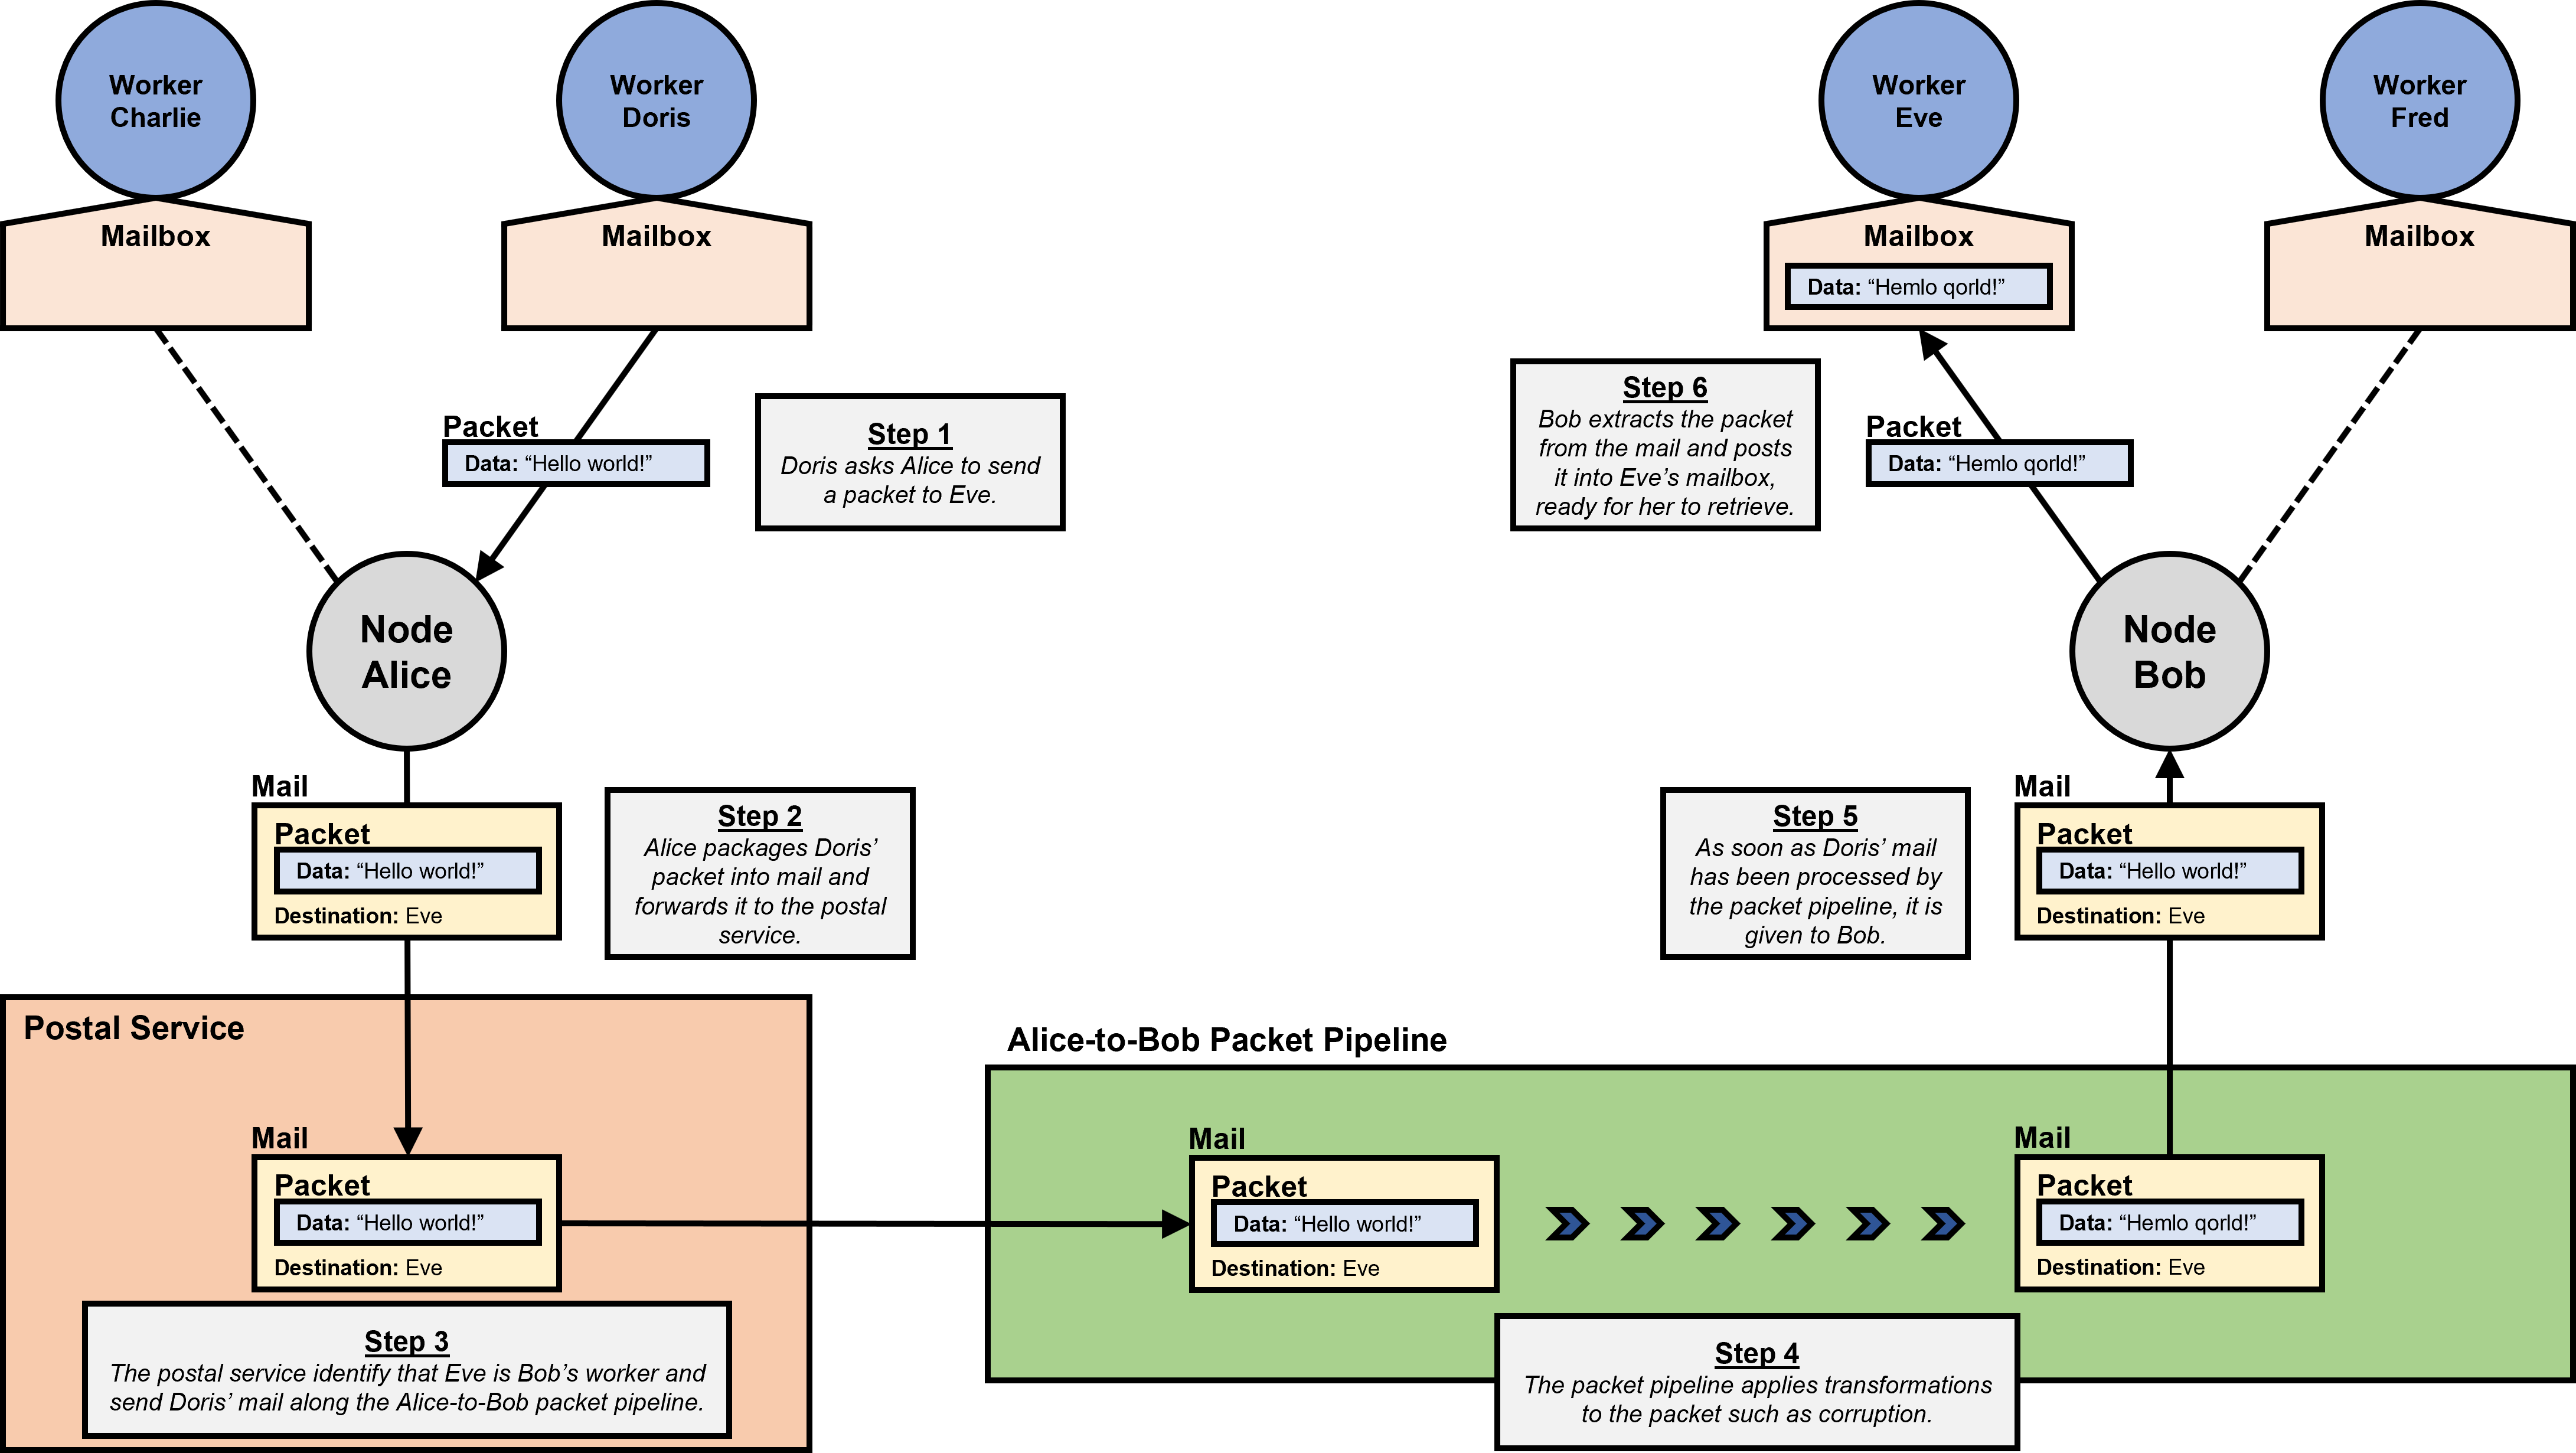
\includegraphics[width=\textwidth]{images/chapter_3_design/simulation_semantics_diagram}
    \centering
    \caption{An example of how a packet would be sent from one worker to another in a Packet Courier simulation
    .}\label{fig:chapter_3_design-simulation_semantics_diagram}
\end{figure}

In this way, workers doing work on a node can be interpreted as a group of machines being connected to a central
router. Machines can connect and disconnect freely to a router, just as workers can be spawned and killed atop a node. A
router provides each of its machines with a unique local ip-address, but has its own ip-address which it shares with
the world, just as is the case with worker and node addresses. Routers are only directly connected to their
neighbours (by definition), and as such, if a device wishes to send a message to a destination that is more than one
degree removed, then it will need to ask intermediate routers to forward the message onward. Once again, Packet
Courier is no different: nodes can only directly send mail to their immediate neighbours.

\newpage

\subsection{Network Condition Semantics}\label{subsection:network_condition_semantics}

\lettrine{W}{hen} it comes to the \emph{network} aspect of the network simulation framework that Packet Courier offers,
\texttt{tc-netem}\cite{tc_netem_wiki, tc_netem_8_man,tc_netem_src} provides an excellent template to draw from.
Indeed, Packet Courier incorporates most of the semantics that \texttt{tc-netem} lays out for itself, just with a few
subtle tweaks, namely:
\begin{itemize}
    \item \textbf{Bandwidth throttling} \\
    Constrains bitrate to a specified upper limit. \\ \\
    \emph{Packet Courier achieves this effect in a very prescriptive manner by imbuing each packet with a latency
    based on the maximum throughput and the size of the packet. For example, if the bitrate was set to 4MBps and a
    1MB packet arrived, then it would be made to wait 0.25 seconds in simulation time. This effect stacks, meaning
    that if a 2MB packet then arrived in the same tick, it would be made to wait 0.75 seconds to account for the 1MB
    of data that is yet to experience its 0.25 seconds of latency. In this way, 3MB is transferred over 0.75 seconds,
        upholding a 4MBps bitrate. \\ \\
        The general premise is to control the bitrate of a connection rather than drop excess packets. Consequently,
        packet throttling does risk becoming a black hole with respect to memory, particularly in cases where a
        high-throughput connection is being heavily throttled over a long period of time. As such, packet throttling
        should mainly be used to smooth out connections that are prone to burst behaviours, rather than as a cheap
        and dirty bitrate control mechanism. This is unlikely to satisfy users on its own, however, and as such, the
        packet throttling semantics include a drop-threshold parameter which acts as a fail-safe: if the number of
        bytes currently held in the packet throttler's buffer exceeds the threshold, then incoming packets will be
        dropped until the contents of the buffer fall below this threshold again.}
    \item \textbf{Packet limiting} \\
    Enforces that only a certain number of packets can be enqueued within a certain time-frame, dropping any that
    exceed the limit. \\ \\
    \emph{Packet Courier leverages the notion of a ``packet-budget'' to decide how many packets should be enqueued
    within a particular time-frame. With each simulation tick, the time between the current simulation time and the
    last tick is measured and multiplied with the maximum number of packets per unit time to calculate the
    packet-budget, i.e.: how many packets are allowed through over the course of the next tick.}
    \item \textbf{Packet delay} \\
    Imbues packets with an artificial latency in keeping with a chosen distribution (uniform, normal or exponential).
    \\ \\
    \emph{Delay semantics are achieved by simply sampling the provided distribution and adding that value onto the
    current simulation time to produce a scheduled ``dequeue'' time. Packets can be stored in a priority queue which
    only releases the top element if the current simulation time has passed the scheduled dequeue time. \\ \\
    The only notably difference being the replacement of the Pareto distribution with the exponential distribution.
    This can be chalked up to the exponential distribution already having been implemented for other use-cases, but
    the Pareto distribution being cut due to time constraints.}
    \item \textbf{Packet drop} \\
    Samples a Bernoulli distribution and drops the packet on success. \\ \\
    \emph{Drop semantics remain the same as \texttt{tc-netem}. Gilbert Elliott and Markov modelling were left out
    because they can be replicated as part of the more general event-based semantics. ``Loss'' has been changed to
    ``drop'' to avoid confusion with notions of corruption.}
    \item \textbf{Packet corruption} \\
    Samples a Bernoulli distribution and flips a random bit on success.\\ \\
    \emph{Corruption semantics remain the same as \texttt{tc-netem}.}
    \item \textbf{Packet duplication} \\
    Samples a Poisson distribution to decide how many duplicates the given packet should have and enqueues that
    number of copies alongside the packet itself. \\ \\
    \emph{Duplication semantics remain the same as \texttt{tc-netem} with the exception that the Bernoulli distribution
    has been generalised to a Poisson distribution. Indeed, if a packet is dropped on the success of a Bernoulli
    sample with parameter $p = 0.42$, then there will be 0.42 duplicate packets on average, as would be the case with
    a Poisson distribution parameterised by $\lambda = 0.42$.}
\end{itemize}

\newpage

\subsection{Event-Based Semantics}\label{subsection:event_based_semantics}

\lettrine{I}{n} addition to simple Bernoulli sampling, \texttt{tc-netem} offers two different stateful methods to
model packet
loss\cite{tc_netem_8_man}:
\begin{itemize}
    \item \textbf{4-state Markov model} \\
    Parameters: \emph{transition probabilities $p13$, $p31$, $p32$, $p23$ and $p14$.} \\
    Semantics: \emph{``State 1 corresponds to good reception, State 4 to independent losses, State 3 to burst losses
    and State 2 to good reception within a burst.''} \\ \\
    This can be thought of more simply as a network boasting two attributes: \emph{reception} and \emph{activity}.
    Reception can either be \emph{good} or \emph{lossy}: if it is good, then packets are not dropped; if it is lossy,
    then packets are dropped. Activity can be either \emph{gap} or \emph{burst} which have no bearing on packet drop
    in isolation. Naturally these two attributes yield a 4-state Markov model as illustrated in
    Figure~\ref{fig:chapter_3_design-tc_netem_4_state_markov_diagram}. \\ \\
    \begin{figure}[!h]
        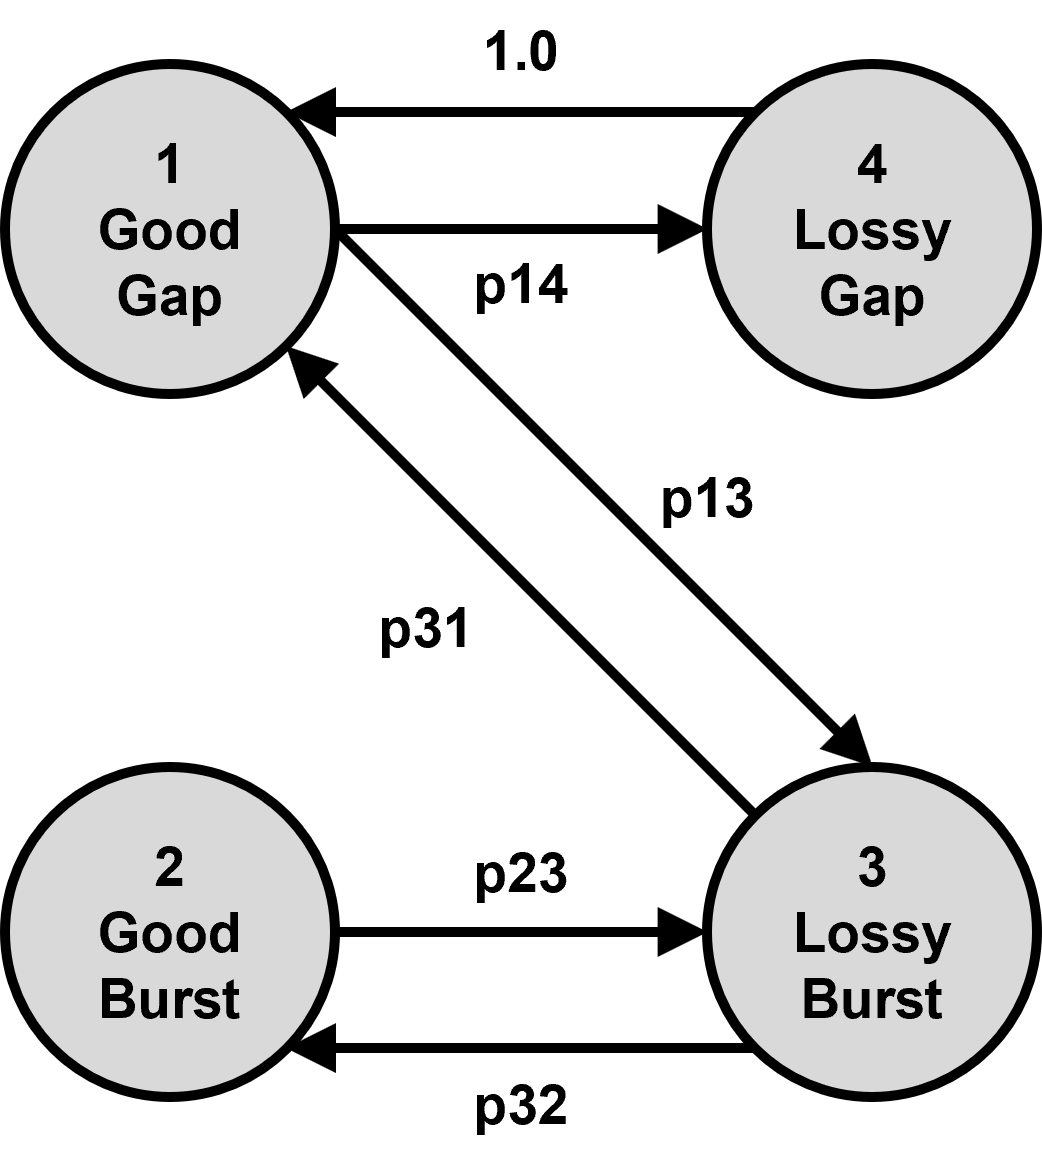
\includegraphics[width=0.35\textwidth]{images/chapter_3_design/tc_netem_4_state_markov_diagram}
        \centering
        \caption{The 4-state Markov packet loss model as implemented by
        \texttt{tc-netem}\cite{tc_netem_src}.}\label{fig:chapter_3_design-tc_netem_4_state_markov_diagram}
    \end{figure}

    The relevance of the activity attribute lies within the fact that the probability of a packet being dropped
    depends on which phase the network is currently undergoing: gap or burst.
    \item \textbf{Gilbert-Elliot loss model} \\
    Parameters: \emph{$p$, $r$, $h$ and $k$.} \\
    Semantics: \emph{``$p$ and $r$ are the transition probabilities between the bad and the good states, $1-h$ is the
    loss probability in the bad state and $1-k$ is the loss probability in the good state.''}
\end{itemize}

\newpage

Whilst these models do give users the opportunity to specify more complex packet drop conditions, they admit of the
following limitations:
\begin{itemize}
    \item \textbf{The 4-state Markov and Gilbert-Elliot models can only be applied to packet drop} \\
    If packet drop can be stateful, then it intuitively follows that other network artefacts can be as well. Indeed,
    one might ask: ``what causes a connection to enter into a `good burst' or a `lossy gap' phase?'' The answer will
    surely relate to underlying quirks of the network infrastructure, which are unlikely to affect loss of packets in
    a manner that is totally independent of latency, say. Even then, plenty of studies have shown (inadvertently or
    otherwise) that network phenomena such as delay and jitter can vary in ways that are seemingly
    stateful\cite{hpbn_mobile_networks, a_close_examination_of_4G_lte_networks,
        gsma_4G_5G_experience_evaluation_guideline, mobile_broadband_networks_under_mobility,
        emulating_3G_4G_networks, study_on_quality_of_service_in_4G_and_5G_networks,
        speed_test_russian_4G_LTE_internet_provider_Beeline}.
    Figure~\ref{fig:chapter_3_design-delay_plotted_against_time_from_study} shows one such example of this principle
    in action, whereby the latency observed appears to behave approximately according to a 3 state model: ``good'',
    where delay seems to mostly hover in the 25-30ms region; ``bad'', where delay will occasionally spike to as high
    as 50ms; ``ugly'', where delay very rarely spikes to even higher than 50ms. To illustrate this hypothesis
    further, we can see similar patterns when examining other metrics such as traffic load, as demonstrated in
    Figure~\ref{fig:chapter_3_design-traffic_load_plotted_against_time_from_study}. \\ \\

    \begin{figure}[!h]
        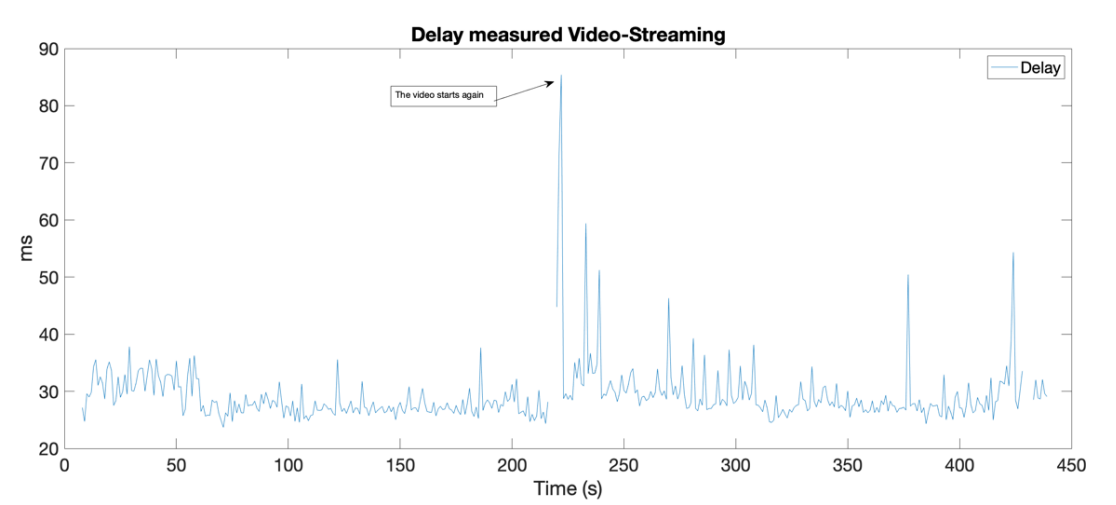
\includegraphics[width=0.9\textwidth]{images/chapter_3_design/delay_plotted_against_time_from_study}
        \centering~\caption{Delay (ms) on 4G packets bent sent as part of a video streaming service \\
        measured over time (s)\cite{study_on_quality_of_service_in_4G_and_5G_networks}.
        }\label{fig:chapter_3_design-delay_plotted_against_time_from_study}
    \end{figure}
    \begin{figure}[!h]
        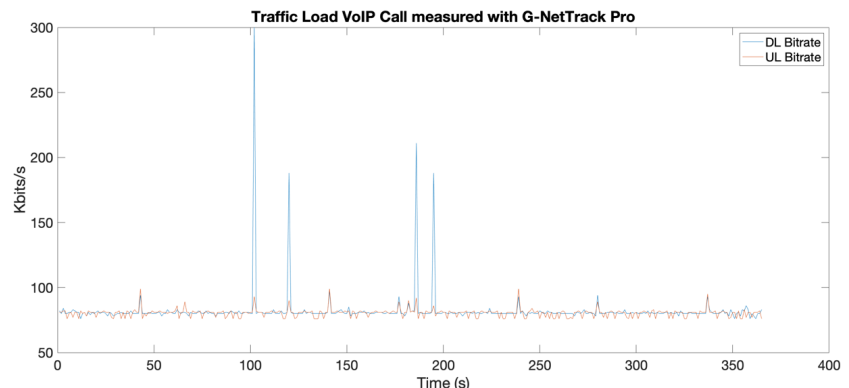
\includegraphics[width=0.9\textwidth]{images/chapter_3_design/traffic_load_plotted_against_time_from_study}
        \centering~\caption{Traffic Load (KBits/s) on 4G packets bent sent as part of a VoIP call measured over
        time (s)\cite{study_on_quality_of_service_in_4G_and_5G_networks}.
        }\label{fig:chapter_3_design-traffic_load_plotted_against_time_from_study}
    \end{figure}

    In this way, one could eyeball the number of states that would be appropriate to model the kind of conditions
    observed in Figures~\ref{fig:chapter_3_design-delay_plotted_against_time_from_study}
    and~\ref{fig:chapter_3_design-traffic_load_plotted_against_time_from_study}, only to then perform some kind of
    k-means clustering algorithm to aggregate the relevant statistics and characterise these states, i.e.: how
    frequently they occur; how long they last; how their key metric (drop, delay, traffic-load) is distributed.
    Notice that we are now in the realm of event-based semantics, where (network) events are being described by their
    interval, duration and effect, which leads nicely onto the second issue with \texttt{tc-netem}'s state-based
    models.
    \newpage
    \item \textbf{Probabilistically parameterised models are hard to reason about} \\
    Consider a network engineer who is new to a particular codebase and finds a protocol testbed with the following
    configuration:
    \begin{quote}
        \texttt{loss p13=0.5 p31=0.25 p32=0.4 p23=0.7 p14=0.15}
    \end{quote}
    There is a distinct likelihood that bafflement would ensue. \\ \\
    Although probabilistic state-based modelling can be very powerful, expressing a virtual network scenario in terms
    of state-transition probabilities does not always lend itself well to being human-readable. Most would find it
    difficult to develop a sense of how the network defined above would behave in even a coarse sense. For example,
    if packets flowed into the simulation at a constant rate, what might the graph of throughput against time look
    like? How would it be shaped? Would there be peaks and troughs, and if so, how frequently and for how long? These
    are important questions that are not necessarily self-evident from a selection of transition probabilities.
    \item \textbf{What if 4-state Markov and Gilbert-Elliot models don't fit the bill?} \\
    Unless a particular network admits of exactly one state, a ``good`` and a ``bad'' state, or four states
    characterised by ``good''/``lossy'' and ``gap''/``burst'', then it'll be a hard task to accurately model it
    using \texttt{tc-netem}. Packet loss on mobile connections has been shown to differ significantly based on locality
    and speed of travel\cite{mobile_broadband_networks_under_mobility}, and with the gaming industry trending towards
    mobile ventures\cite{statista_mobile_gaming, rise_of_mobile_gaming}, there is a strong chance that game development
    firms will want to optimize their net-code by emulating the kind of network conditions experienced when on a
    train, bus or car journey. As such, a more general purpose set of semantics are required for undertakings of this
    nature.
\end{itemize}

\newpage

These limitations can be overcome by generalising the 4-state Markov and Gilbert-Elliot models into a discrete
event-based model\cite{discrete_event_simulation}. Packet Courier achieves this by incorporating an \emph{event
pipeline} into the core network condition semantics alongside bandwidth throttling, packet delay etc.

An event pipeline consists of a ``default'' set of network conditions and a list of possible network events.
Naturally, the default network conditions are what the pipeline will revert to when no network events are currently
underway. Network events are characterised by their mean interval and duration, as well as what network conditions
they will impose on the simulation. In instances where multiple events have been triggered at the same time, the
conditions with the highest precedence will take priority. Event start and finish times are randomly generated according
to the exponential distributions $Exp(1/\mu_{interval})$ and $Exp(1/\mu_{duration})$ respectively. The
exponential distribution is not an arbitrary choice, since it is the only continuous distribution that boasts a
\emph{memoryless} property\cite{memoryless_random_variables}. Indeed, discrete event simulations are built upon
principles of memorylessness, namely because it ensures that sampled intervals and durations do not crudely depend on
the time that has already elapsed. This is crucial since events are often best modelled as being independent of one
another, insofar as an event would be scheduled in a way that is ignorant of previous events in the simulation. In a
real-world context, one can imagine a dip in 4G service being caused by a bus going underneath a bridge: would the
event of ``going under a bridge'' be described as an \emph{independent} occurrence? The answer is almost certainly
``yes''. Note however that an event pipeline is itself a network condition, so a network event could in principle
invoke a new event pipeline (only for the duration of the event, of course). This does then provide scope for
network events to ``depend'' on one another via the use of nested pipelines.

It is also no coincidence that the discrete memoryless distribution is geometric\cite{memoryless_random_variables},
not only because this is essentially the ``floored'' version of the exponential distribution, but it is used to
convert a set of state transition probabilities into discrete event parameters. Let us refer back to
Figure~\ref{fig:chapter_3_design-tc_netem_4_state_markov_diagram} as the subject for a worked example.

Let us first assume that a state transition occurs once per tick, which simply corresponds to an arbitrary unit of
time. The mean ``duration'' of each state can be computed by evaluating the expected number of consecutive ticks
without state change for each individual state. It follows that this would be distributed geometrically with the
parameter $p$ set to the probability of a state change. Hence, the mean durations for each state in
Figure~\ref{fig:chapter_3_design-tc_netem_4_state_markov_diagram} are as follows:
\begin{align*}
    \mu_{1,duration} &= \frac{1}{1 - p_{13} - p_{14}} \\
    \mu_{2,duration} &= \frac{1}{1 - p_{23}} \\
    \mu_{3,duration} &= \frac{1}{1 - p_{31} - p_{32}} \\
    \mu_{4,duration} &= 1
\end{align*}

The mean ``interval'' of each state can be similarly computed by evaluating the expected number of consecutive ticks
whereby the simulation is not in that particular state. This random variable would be distributed geometrically with
the parameter $p$ set to the probability that a state transition is not directed towards the state in question,
given that the prior state was also not the state in question. Using state 1 in
Figure~\ref{fig:chapter_3_design-tc_netem_4_state_markov_diagram} as an example, $p$ in this case would be the
probability that the simulation transitioned to state 2, 3 or 4, given that it was already in one of those states
prior. Hence, the mean intervals for each state in Figure~\ref{fig:chapter_3_design-tc_netem_4_state_markov_diagram}
are as follows:
\begin{align*}
    \mu_{1,interval} &= \frac{q_2 + q_3 + q_4}{q_2 + q_3(1 - p_{31})} \\
    \mu_{2,interval} &= \frac{q_1 + q_3 + q_4}{q_1 + q_3(1 - p_{32}) + q_4} \\
    \mu_{3,interval} &= \frac{q_1 + q_2 + q_4}{q_1(1 - p_{13}) + q_2(1 - p_{23}) + q_4} \\
    \mu_{4,interval} &= \frac{q_1 + q_2 + q_3}{q_1(1 - p_{14}) + q_2 + q_3}
\end{align*}

Where $q_i$ is the probability that the simulation is in state $i$ at any given time, which can be solved by the
following homogenous system:
\begin{align*}
    q_1 &= q_1(1 - p_{13} - p_{14}) + q_3p_{31} + q_4 \\
    q_2 &= q_2(1 - p_{32}) + q_3p_{32} \\
    q_3 &= q_1p_{13} + q_2p_{23} + q_3(1 - p_{31} - p_{32}) \\
    q_4 &= q_1p_{14}
\end{align*}

The purpose of this exercise is to illustrate the relationship between state transitional models and Packet Courier's
event-based semantics. In fact, one could generalise the above process into a set of formulaic linear equations and
hence write an algorithm to convert state transition probabilities into their respective mean durations and
intervals. This observation serves less as a proposition for a potential feature, and a more rigorous demonstration
that the semantics laid out in this section subsume the models available within the \texttt{tc-netem} framework,
converting them into a format that is more easily read and understood by humans.

\newpage

\subsection{Algorithms}\label{subsection:algorithms}

\lettrine{M}{ost} of the Packet Courier semantics as defined up until this point should map more or less directly onto a
programmed implementation. There are a few instances where this isn't the case, however, namely when sampling the
statistical distributions which sit at the heart of Packet Courier's network simulation. The normal and Poisson
distributions are particularly problematic since neither has a closed form inverse cumulative distribution function,
ergo neither can be trivially sampled by percentile.

\subsubsection{Normal Distribution Sampler}\label{subsubsection:normal_distribution_sampler}

The Box-Muller transform converts a pair of independent, uniform, random variables, $U_1, U_2 \sim U(0, 1)$ into a pair
of independent, normal, random variables $Z_0, Z_1 \sim \mathcal{N}(0, 1)$\cite{box_muller_transform} via the
following process: \\

\begin{algorithm}[caption={Box-Muller Transform\cite{box_muller_transform}.},label={alg:box_muller_transform},
    captionpos=b]
    $U_1 \gets$ sample $U(0, 1)$
    $U_2 \gets$ sample $U(0, 1)$
    $R \gets \sqrt{-2 log_e U_1}$
    $\theta \gets 2 \pi U_2$
    $Z_0 \gets R \cos \theta$
    $Z_1 \gets R \sin \theta$
\end{algorithm}

Note that this algorithm would only need to be run every other sample, since it generates two standard normal
variables. Moreover, it can be readily be adapted to any arbitrary normal distribution, since $Z \sim \mathcal{N}(0,
1) \implies \mu + \sigma Z \sim \mathcal{N}(\mu, \sigma^2)$.

\subsubsection{Poisson Distribution Sampler}\label{subsubsection:poisson_distribution_sampler}

The Poisson cumulative distribution function for $X \sim Poi(\lambda)$ as defined as follows:
\begin{align*}
    F_X(x) = e^{-\lambda} \sum_{i=0}^{\lfloor x \rfloor} \frac{\lambda^i}{i!}
\end{align*}

\begin{figure}[!h]
    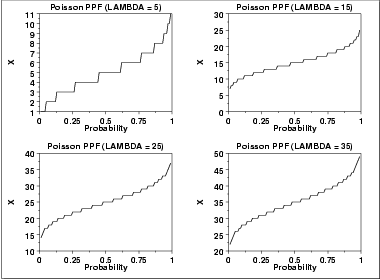
\includegraphics[width=0.9\textwidth]{images/chapter_3_design/poisson_percent_point_function}
    \centering~\caption{The inverse CDF (or PPF: percent point function) of the Poisson distribution for various
        $\lambda$ parameters\cite{engineering_statistics_handbook_poisson_distribution}.}
    \label{fig:chapter_3_design-poisson_percent_point_function}
\end{figure}

As such, $F_X(x)$ sketches a step graph delimited by $x \in \mathbb{N}$ as illustrated by
Figure~\ref{fig:chapter_3_design-poisson_percent_point_function}. This property makes the Poisson distribution
perfect for tabulation, whereby the sampling strategy is to pre-compute a reasonable selection of percentile-value
pairs (i.e.: percentiles between 0 and 0.999) and perform simple lookups based on a uniform random percentile sample
$U \sim [0, 1)$.

\newpage

\begin{algorithm}[caption={Poisson distribution builder and sampler.},label={alg:poisson_builder_and_sampler},
    captionpos=b]
    function builder_poisson_table($\lambda$):
    $\quad$ $term \gets e^{-\lambda}$
    $\quad$ $percentile \gets 0$
    $\quad$ $x \gets 0$
    $\quad$ $table \gets$ new table()
    $\quad$ while $(1 - percentile) > \epsilon$ do
    $\quad$ $\quad$ add $\langle percentile, x \rangle$ to table
    $\quad$ $\quad$ $x \gets x + 1$
    $\quad$ $\quad$ $percentile \gets percentile + term$
    $\quad$ $\quad$ $term \gets term \cdot \frac{\lambda}{x}$
    $\quad$ end
    $\quad$ add  $\langle 1, x \rangle$ to table
    $\quad$ return table
    end

    function sample_poisson_table(table):
    $\quad$ $percentile \gets$ sample $U[0, 1)$
    $\quad$ $\langle lower, upper \rangle \gets$ lookup $percentile$ in table
    $\quad$ # $lower$ is the table entry where $lower.percentile$ is the
    $\quad$ # largest percentile that is smaller than the lookup parameter.
    $\quad$ # $upper$ is the converse of $lower$.
    $\quad$ # Taking $lower.x$ mimics the flooring behaviour of $F_X(x)$.
    $\quad$ return $lower.x$
    end
\end{algorithm}


\section{Top-Down Specification}\label{section:top_down_specification}

\lettrine{N}{ow} that Packet Courier's core simulation and network semantics have been established, the next
important consideration is how this proposed functionality will be delivered to users. The path of least resistance
is to implement the framework in a way that is highly accessible for programmers to immediately interface with. From
there, more complex features can be built on top of this initial API to broaden the scope of the tool ad hoc.

\subsection{Application-Programmer Interface}\label{subsection:application_programmer_interface}

\lettrine{A}{t} the bare minimum, a Packet Courier simulation needs to be provided with the following parameters:
\begin{itemize}
    \item The topology of the simulated network.
    \item A set of ``scripts'' which run atop each node in the simulated network.
    \item The simulated network conditions for each node-to-node connection.
\end{itemize}

The simplest way of enabling the user to define these aspects of the simulation would be to provide them with an
API capable of the following:
\begin{itemize}
    \item Create a blank simulation configuration.
    \item Add a new, uniquely named node to a configuration.
    \item Imbue a node with a runnable ``script''.
    \item Connect two nodes with a set of network conditions.
    \item Run a configuration as a simulation.
\end{itemize}

The notion of a ``script'' which runs on each node has been quite vague thus far. The general premise would be to
spawn a root worker within each node on simulation startup, and provide them with a user defined code snippet which
will set them to work. This then presents the problem of how the user is expected to write code which interfaces with
the details of the simulation ahead of time. Alas, a worker needs to be given the autonomy to know its own address,
send packets to other workers, extract packets from its own mailbox, spawn its own child workers, etc. How can a user
take advantage of these features using a pre-programmed ``script'' that write when configuring their simulation?

Packet Courier overcomes this obstacle by modelling a \emph{Worker-Script} as a lambda that takes a
\emph{Worker-Manager} as a parameter. A worker-manager can be thought of as a collection of lambdas that together
capture the capabilities of a worker. The fact that a worker-script is a lambda allows a user to write code whilst
manipulating an arbitrary parameter which in turn provides the requisite context.
Algorithm~\ref{alg:worker_script_example} illustrates this principle in action. \\

\begin{algorithm}[caption={An example of what a worker-script might look like.},label={alg:worker_script_example},
    captionpos=b]
    function alice_worker_script(worker_manager):
    $\quad$ $neighbour \gets$ worker_manager.get_neighbour()
    $\quad$ $packet \gets$ "Hello neighbour! My name is Alice." as bytes
    $\quad$ worker_manager.send_mail($neighbour$, $packet$)
    $\quad$ $packet \gets$ worker_manager.wait_for_mail()
    $\quad$ $message \gets packet$ as string
    $\quad$ worker_manager.log($message$)
    end
\end{algorithm}

Notice that the worker-script in Algorithm~\ref{alg:worker_script_example} takes advantage of a function called
\texttt{get\_neighbour}. This then raises the question of what information should workers be provided with? Of course,
they should still be provided with the basic functionality of knowing their own address, sending and receiving mail,
spawning child workers and logging messages, but what \emph{information} should they be given regarding the wider
simulation? Should they know the addresses of their neighbours? Or should they be given a blueprint of the entire
topology? How about a random subset? Should workers be able to see the current simulation time as well?

The answer to all of these questions depends on the use-case of the simulation and should ideally be decided by the
user themselves. Packet Courier achieves this using a ``care package'' style system, i.e.: a worker-manager can
provide a package of information on request, where the exact contents of this package have been defined ahead of
time by the user. This too takes advantage of a lambda called a \emph{Node-Info Generator}, which takes a snapshot of
the simulation as its parameter and processes it into a bespoke care package which workers can enjoy. This
``generation'' of node-info is only done once per node on simulation startup in case it happens to be an
intensive procedure. In this way, the call to \texttt{get\_neighbour()} on line 2 of
Algorithm~\ref{alg:worker_script_example} should in reality be something like \texttt{get\_info().get\_neighbour()}.

In summary, if a user wished to leverage this conceptual Packet Courier API, they would write some code that looked
something akin to Algorithm~\ref{alg:simulation_configuration_example}; the logged output would be:
\begin{quote}
    \texttt{> Hello neighbour! My name is Alice.} \\
    \texttt{> Greetings! I am Bob.}
\end{quote}

\newpage

\begin{algorithm}[caption={An example of what configuring a simulation might look like.},
    label={alg:simulation_configuration_example},
    captionpos=b]
    function bob_worker_script(worker_manager):
    $\quad$ $packet \gets$ worker_manager.wait_for_mail()
    $\quad$ $message \gets packet$ as string
    $\quad$ worker_manager.log($message$)
    $\quad$ $neighbour \gets$ worker_manager.get_neighbour()
    $\quad$ $packet \gets$ "Greetings! I am Bob." as bytes
    $\quad$ worker_manager.send_mail($neighbour$, $packet$)
    end

    $config \gets$ new config()
    add ("Alice" using $alice\_worker\_script$) to $config$
    add ("Bob" using $bob\_worker\_script$) to $config$
    $network\_conditions \gets$ new network_conditions()
    add (uniform packet drop from 35 to 50 in ms) to $network\_conditions$
    add ($network\_conditions$ from "Alice" to "Bob") to $config$
    add ($network\_conditions$ from "Bob" to "Alice") to $config$
    $simulation \gets$ start $config$
    wait for $simulation$ to end
\end{algorithm}

\subsection{Emulation Semantics}\label{subsection:emulation_semantics}

\lettrine{A}{lthough} Packet Courier would be able provide value to users via APIs, it would likely alienate many
developers who were not already using the same programming language as the Packet Courier framework. Forcing
prospective users to write their simulation code in a particular language is diametrically opposed to objectives 4.b)
and 5.a).

Packet Courier solves this issue by taking advantage of its own APIs to build an adaptive interface that generalises
the simulation semantics further to integrate with any arbitrary packet. Indeed, another step has been taken to
evolve the tool once more from a \emph{simulator} to an \emph{emulator}.

Imagine a game developer, Todd, who wants to test his custom networking protocol, SkyNet, for client-server
connections. Todd has built his protocol on top of UDP, since speed is more important than quality of service in the
context of his game. Naturally, there is no real point in conducting vanilla tests on his machine, because the UDP
packets will just be internally routed by the kernel, giving Todd no understanding of how his protocol would perform
in the wild. Todd could use Packet Courier to \emph{emulate} such a scenario, but how?

Todd could leverage the simulation semantics of Packet Courier to set up a topology with two nodes, each adorning a UDP
socket. The worker at these nodes would do carry out two jobs:
\begin{itemize}
    \item Forward packets received by the UDP socket to the other worker.
    \item Send packets in the mailbox onward to the client/server via the UDP socket.
\end{itemize}

Notice however that there are now four UDP sockets in play: the client's, the server's and the two being used by
Packet Courier. As a consequence, Packet Courier needs to perform some sleight of hand here and essentially lie to
the client and the server about the ip-address of their counterpart. Thus, the client and the server will actually
end up sending their packets to Packet Courier whilst thinking that they are sending them directly to each other.

In the case where Todd wanted to test his game using multiple clients to a single server, then the exact same
principle applies. The only difference is that Packet Courier would need to keep track of which ip-addresses
corresponded to which node.

To formalise these semantics, Packet Courier is said to use an abstraction of ``public'' vs ``private'' ip-addresses in
order to slot the emulated network inbetween running processes. Each process is assigned a private ip-address which
corresponds to the address it should be sending and receiving packets on. Whilst processes could just communicate purely
using these ip-addresses, they would simply be passing messages using UDP as a protocol and the operating system
kernel as a wire; there would be no scope for manipulating the transmission of packets in a way that mimics a
particular type of internet connection.

To solve this problem, Packet Courier introduces the notion of a public ip-address, which allows Packet Courier to
intercept packets and modify them as per the user configuration. By way of analogy, one could think of a private
ip-address as a home address and a public ip-address as a PO Box. Suppose someone doesn't want mail to be sent
directly to their home for whatever reason; in this instance they can open a PO Box, whereby they collect parcels and
letters that they know are intended for them in an environment where they can be screened and processed.

\begin{figure}[!h]
    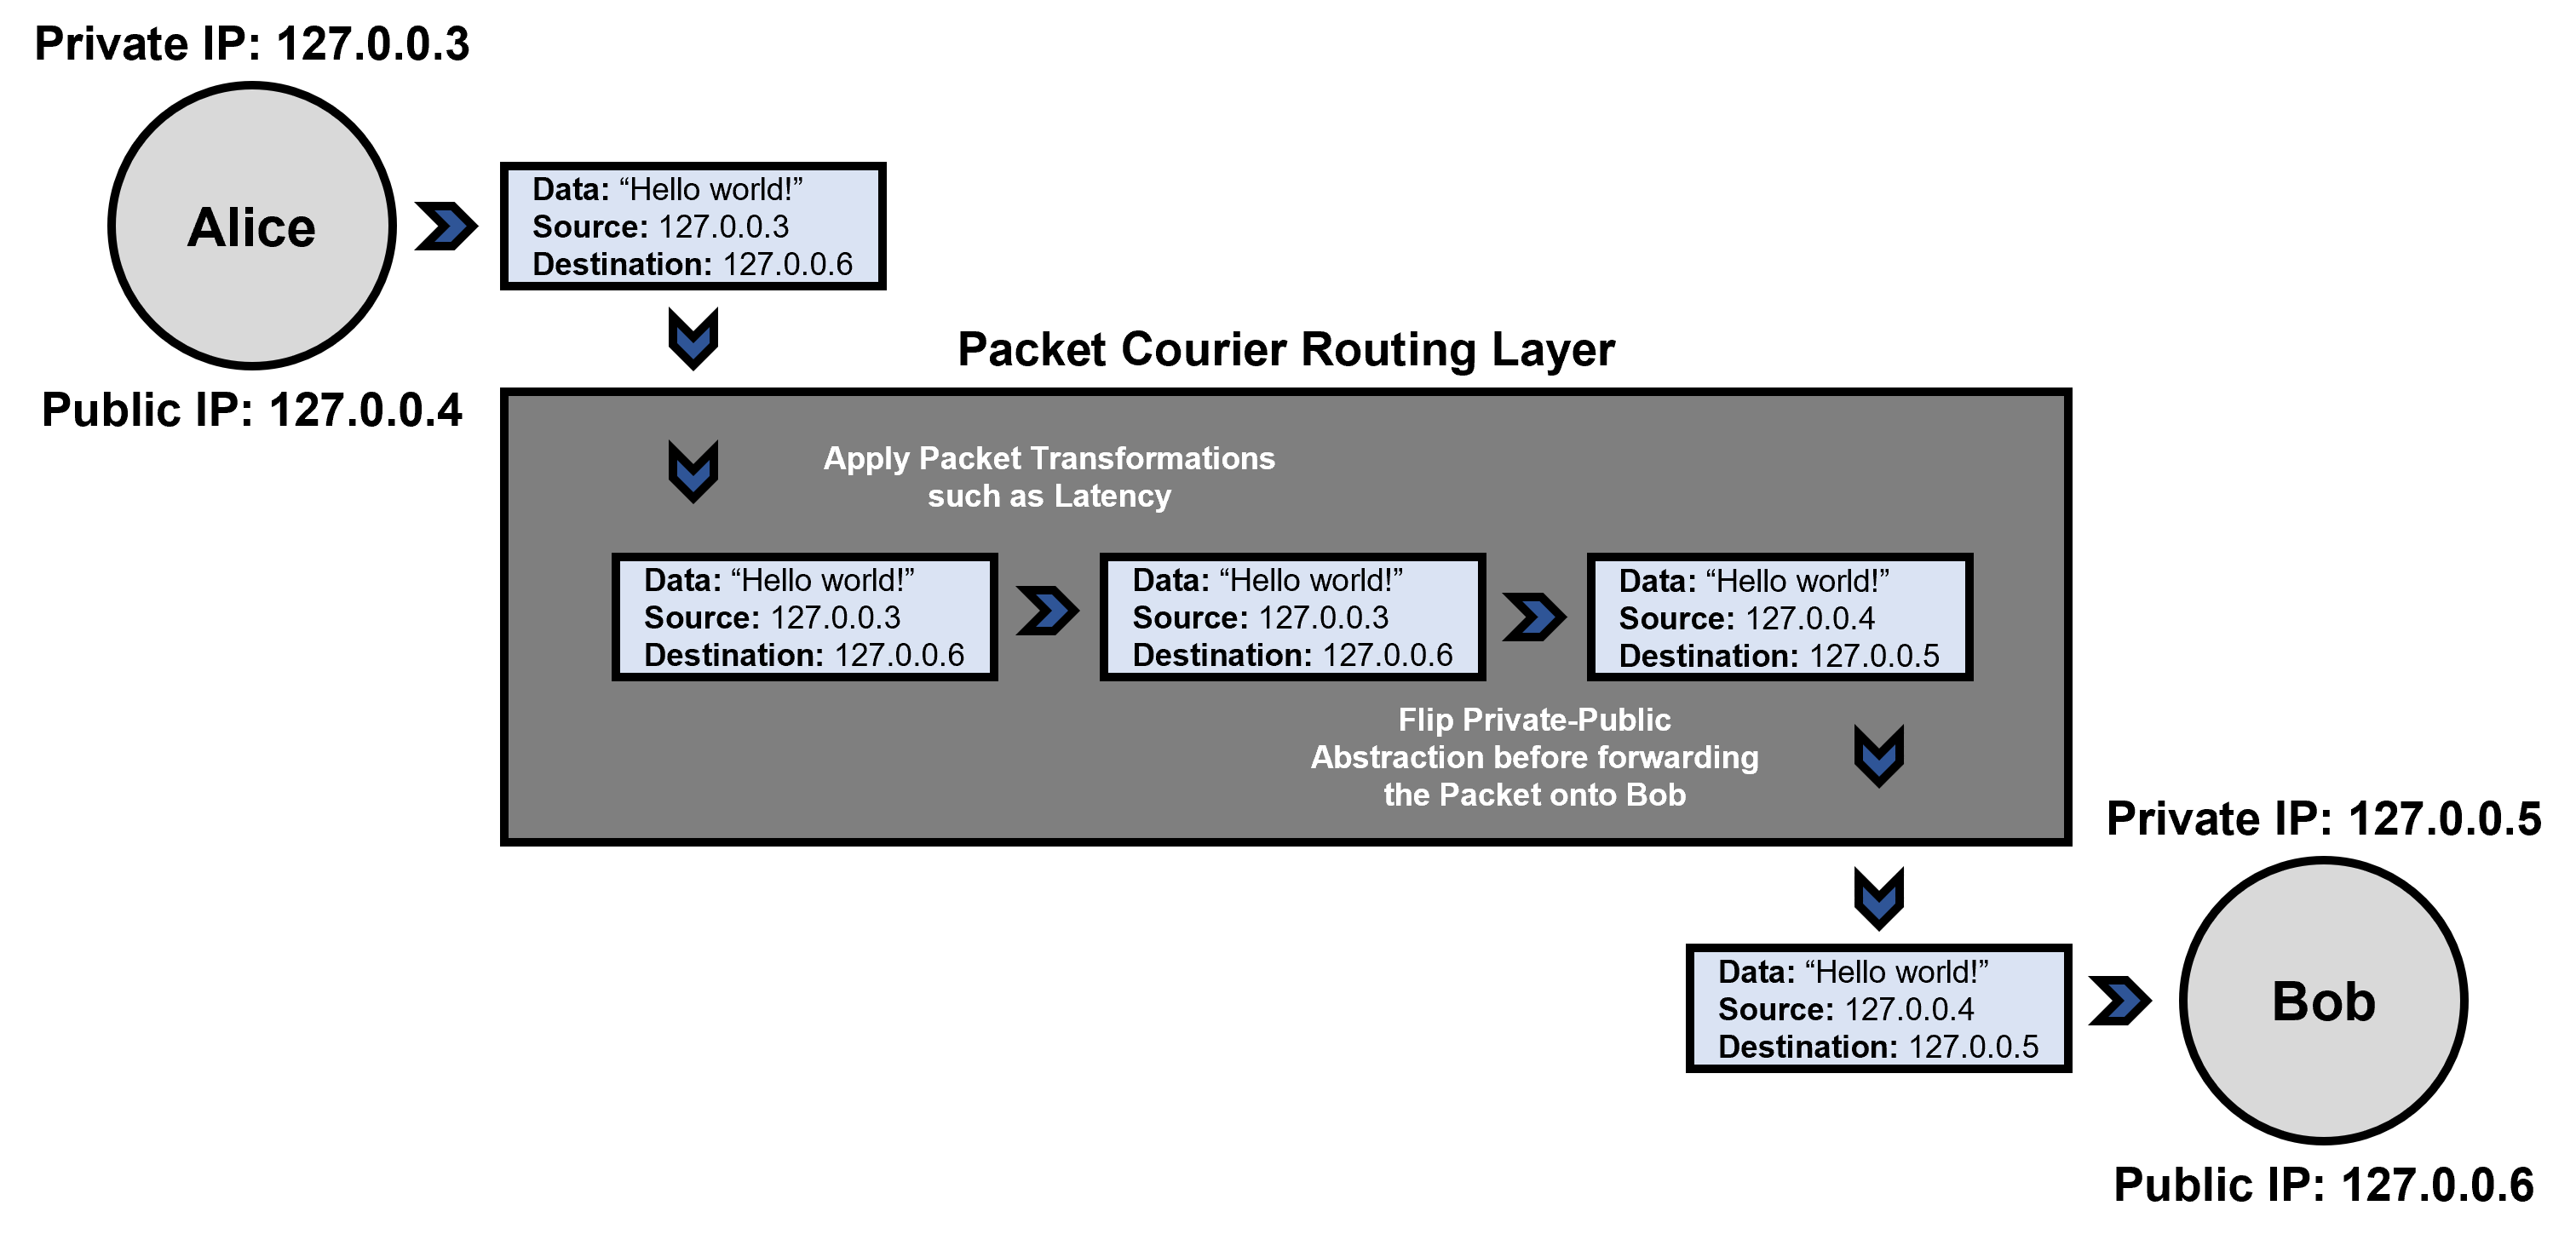
\includegraphics[width=\textwidth]{images/chapter_3_design/emulation_semantics_diagram}
    \centering~\caption{A diagram demonstrating how Alice sends a packet to Bob.}
    \label{fig:chapter_3_design-emulation_semantics_diagram}
\end{figure}

For example, consider bidirectionally connected nodes Alice and Bob (as in
Figure~\ref{fig:chapter_3_design-emulation_semantics_diagram}). Alice is told at runtime that her private ip-address is
\texttt{127.0.0.3}, her public ip-address is \texttt{127.0.0.4} and she is neighboured with Bob who has a public
ip-address of \texttt{127.0.0.6}. When Alice wants to send a packet to Bob, she should send it from her private UDP
socket with address \texttt{127.0.0.3} to the destination of \texttt{127.0.0.6}. Alice will in fact be sending her
packet to the Packet Courier routing layer, which will determine that this is Alice attempting to send a packet to
Bob, in turn applying any network conditions such as latency, loss and corruption to the packet, before forwarding it
on to Bob's private ip-address, ensuring that the source is listed as Alice's public ip-address.

One potential issue with this approach is that nodes could (accidentally or otherwise) simply pass on their private
ip-address and have other nodes bypass the emulator entirely. There is of course nothing that can realistically be
done to stop this, in the same way that there is nothing stopping users from hard coding ip-addresses into their
protocols which would have a similar effect. Ideally Packet Courier would manipulate packets at the level of the
kernel, bypassing the need for this architecture in the first place, however this just isn't very feasible in a way
that is portable, containerised and platform-agnostic. Thus, this is just a limitation that users should be
encouraged to bear in mind when using the tool.

In conclusion, Packet Courier's emulation semantics enable arbitrary processes to interface with Packet Courier
using UDP. Given that virtually every networking protocol will ultimately use UDP at the lowest-levels of
abstraction, this opens up Packet Courier to be used in real-world contexts with minimal setup. Indeed, Packet
Courier can be used as a standalone emulator and invoked from the command-line without writing a single line of
simulation code.



%chapter 4 formatting


    \chapter{Implementation}
    \pagestyle{fancy}
    \fancyhf{}
    \rhead{\small Implementation}
    \lhead{\small Chapter 4}
    \rfoot{\thepage}
    \lfoot{\small MEng Project}
    \renewcommand{\headrulewidth}{2pt}
    \renewcommand{\footrulewidth}{2pt}
    \section{Project Management}

\subsection{Version Control}

Packet Courier was developed using Git\cite{git} as a version control system and the code repository is hosted on
GitHub\cite{github, packet_courier} at \url{https://github.com/thelukethorpe/packet_courier}. There is no special
reason for either of these choices; they are simply industry standards being used for a project that doesn't
innately demand bespoke tooling (unlike data-heavy ventures such as game development, which might benefit from a tool
like Perforce\cite{perforce, perforce_vs_git}).

\subsection{Ticket Tracking}

GitHub Issues\cite{github_issues} powers Packet Courier's ticket tracking. Tickets, or \emph{issues}, as per the
GitHub nomenclature, are categorised based on one or more of the following custom tags:
\begin{itemize}
    \item \textbf{Bug:} \emph{Something isn't working.}
    \item \textbf{CI:} \emph{Change to pipeline.}
    \item \textbf{Documentation:} \emph{Improvements or additions to documentation.}
    \item \textbf{Feature:} \emph{New feature or request.}
    \item \textbf{Optimization:} \emph{Improvements in performance.}
    \item \textbf{Refactor:} \emph{Tech-debt, structural change of quality-of-life improvement.}
    \item \textbf{Testing:} \emph{Improvements or additions to test suite.}
    \item \textbf{Won't Fix:} \emph{This will not be worked on.}
\end{itemize}

Issues are further organised using a Kanban board\cite{kanban_board}. As the \emph{documentation} tag suggests,
this board is not only used for development purposes, in fact, it has been used to help manage the project
holistically, including the writing of this very report, as shown in
Figure~\ref{fig:chapter_4_implementation-github_kanban_board}.

\begin{figure}[!h]
    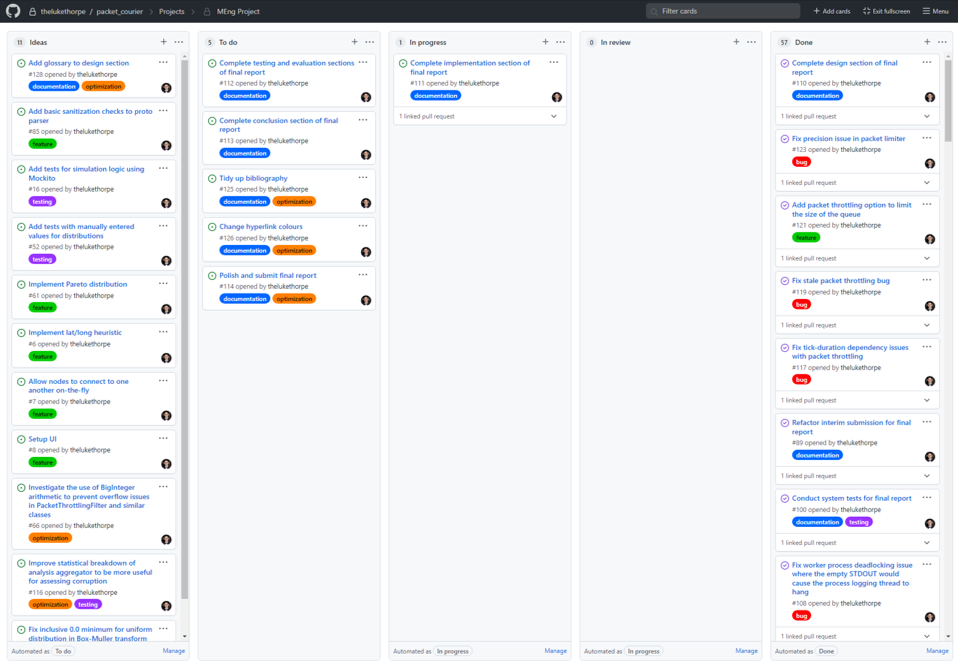
\includegraphics[width=\textwidth]{images/chapter_4_implementation/github_kanban_board}
    \centering~\caption{Packet Courier's Project Kanban Board\cite{packet_courier}.}
    \label{fig:chapter_4_implementation-github_kanban_board}
\end{figure}

Pull-requests are opened for every merge to the \texttt{main} branch and linked to the associated ticket number.
Branches are named with a uniform and consistent structure, prefixed by the issue number followed by a brief subtitle
of the ticket delimited by hyphens. Despite being an individual project, this repository has been maintained to
industry standards of software engineering practices for organisational reasons, and has in turn benefited massively
from it.

\begin{figure}[!h]
    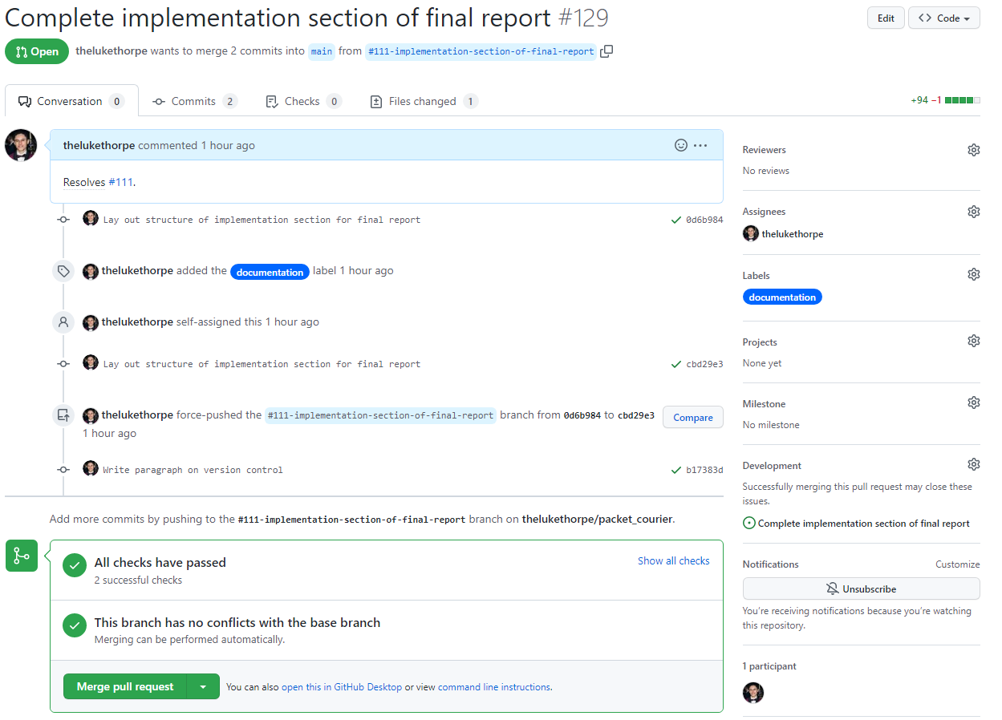
\includegraphics[width=\textwidth]{images/chapter_4_implementation/github_pull_request}
    \centering~\caption{An example of a pull-request in the Packet Courier repository\cite{packet_courier}.}
    \label{fig:chapter_4_implementation-github_pull_request}
\end{figure}

\newpage

\subsection{Programming Languages}

Java 8\cite{java_8} was chosen as the foundational language for Packet Courier due to:
\begin{itemize}
    \item Its excellent breadth of supported platforms\cite{java_8_support}, which lends itself well to objective 4.a).
    \item The vast number of popular and easily importable libraries available to it\cite{java_relevance}.
    \item Its object-oriented nature, which maps nicely onto the abstract semantics laid out in the design section.
    \item Its relatively high levels of time-efficiency, as shown in
    Figure~\ref{fig:chapter_4_implementation-programming_language_comparison}.
    \item Its suite of concurrency abstractions\cite{java_util_concurrent}.
\end{itemize}

\begin{figure}[!h]
    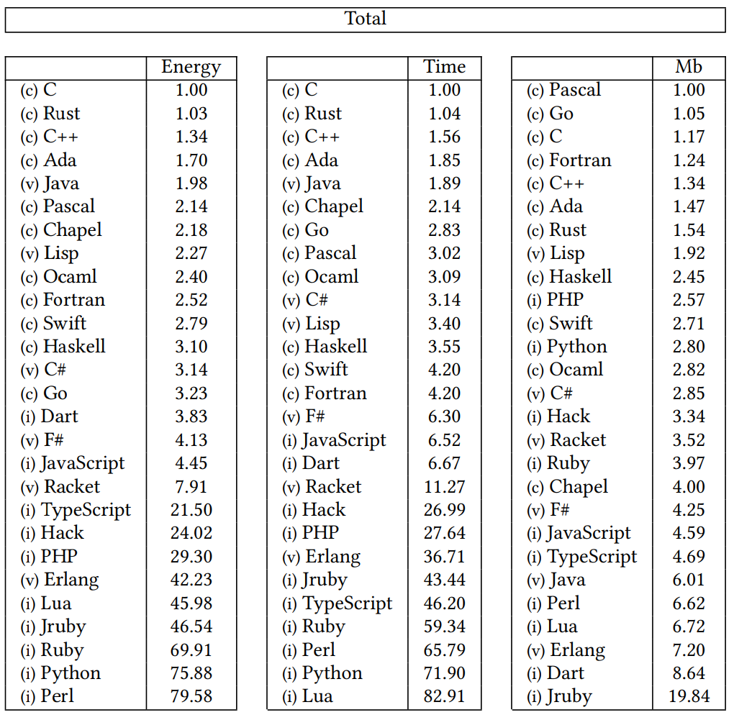
\includegraphics[width=\textwidth]{images/chapter_4_implementation/programming_language_comparison}
    \centering~\caption{A comparison of programming languages based on energy usage, time and memory
    efficiency\cite{programming_language_efficiency}.}
    \label{fig:chapter_4_implementation-programming_language_comparison}
\end{figure}

Although languages such as C and C++ outperform Java across all metrics displayed by
Figure~\ref{fig:chapter_4_implementation-programming_language_comparison}, they are needlessly low-level to the point
where it would likely become a hindrance. Even a cursory investigation into the nature of socket programming in C++
revealed a perfect case study as to the benefits of Java for a problem statement like Packet Courier's. It turns out
that Windows does not natively support the standard C++ socket specification, \texttt{sys/socket.h}, meaning that
\texttt{winsock2.h} must be used instead\cite{socket_vs_winsock}. This would then mean either going to the effort of
implementing two different platform-dependent solutions, or using a library that promises platform agnosticism. There
are many such libraries however\cite{c++_socket_libraries}, placing a substantial research burden on the development
of what should be a fairly simple component. C++ furthermore has been shown to have several non-trivial cross-platform
and cross-compiler discrepancies for even the most basic code\cite{c++_cross_compiler_differences,
    c++_statistical_differences, c++_random_differences, c++_filesystem_differences}.

A key benefit of Java is that it smooths out cross-platform issues, providing developers with a clean, uniform and
highly reliable set of semantics that transcend the nuances of the native operating system and hardware
micro-architecture. Indeed, Java handily has a \texttt{DatagramSocket} class\cite{java_DatagramSocket} which has
proven extremely useful in implementing Packet Courier's standalone emulator. In this way, external Java libraries
are only called-in for more heavyweight or highly specific work, as opposed to routine or menial implementations.

Java also strikes a Goldilocks-esque balance\cite{goldilocks_effect} between low-level languages like C++ and
languages that are arguably even more abstract than Java, such as Python. Whilst Packet Courier does leverage Python
3\cite{python_3} for basic client-server scripts to demonstrate the functionality of the emulator, production code
consists exclusively of Java. Python's dynamic typing\cite{python_typing}, poor
performance\cite{programming_language_efficiency} and inefficient multi-threading and synchronisation
primitives\cite{python_gil} are the main reasons why it wasn't used more prominently within Packet Courier.

\subsection{Build and Dependency Management}

Packet Courier uses Apache Maven 3.6.3\cite{maven} to manage its build phases and dependencies. Maven is convienent,
lightweight, widely supported, boasts a huge repository of libraries\cite{maven_repository} and with a single
command can compile the project into a portable \texttt{.jar} file that can be used as an executable binary or a Java
library.

\subsubsection{JUnit 4}

JUnit 4\cite{juint4} is an industry standard for conducting tests in Java, with an estimated 30.7\% of Java projects on
GitHub using JUnit (according to a study done in 2013)\cite{java_library_popularity}. Naturally, the Packet Courier
unit tests are implemented using JUint 4.13 and are run on each Maven build.

\subsubsection{AssertJ}

AssertJ\cite{assert_j} is used in conjunction with JUnit to provide unit tests with expressive, human-readable checks
such as:

\begin{lstlisting}[language=Java]
public class PacketTest {
  // JUnit 4 test.
  @Test
  public void testPacketStringConversion() {
    String message = "hello there!";
    Packet messageAsPacket = Packet.of(message);
    // AssertJ assertion reads like an English sentence.
    assertThat(messageAsPacket.tryParse()).hasValue(message);
  }

  // Some more tests...
}
\end{lstlisting}

The following paragraph from a \emph{JavaZone} article summarises why AssertJ was favoured over the JUnit default
assertion framework known as Hamcrest\cite{assert_j_vs_hamcrest}:
\begin{quote}
    \emph{``AssertJ is not as well-known as Hamcrest, but at the same time, its popularity has been growing pretty
    fast over the last few years. As opposed to Hamcrest’s classic assertion syntax, which was inherited from the
    default Java testing framework JUnit, the main idea of AssertJ is that it provides fluent syntax. The main goal
    of that is to improve code readability. It’s worth mentioning that AssertJ is a fork of the FEST Assert project,
        which was the first step of AssertJ creation.''}
\end{quote}

\subsubsection{Google Protocol Buffer}

Google Protocol Buffer\cite{google_protobuf} is a multi-faceted library that is supported across multiple languages,
but is used by Packet Courier to parse configuration files into Java objects. There are many file parsing libraries
for specific file formats, such as Google Gson, a Java JSON parsing library\cite{google_gson}. The unique selling
point of Google Protocol Buffer is its neatly compartmentalised workflow:
\begin{enumerate}
    \item Write a \texttt{.proto} file that defines the expected file structure. See
    Code-Snippet~\ref{code:google_protocol_buffer_example} for an example.
    \item Compile the \texttt{.proto} file using Maven to generate the corresponding parse-tree in Java.
    \item Choose a parser such as \texttt{JsonFormat} to generate a parse-tree from an input file.
    \item Perform a semantic pass over the parse-tree, i.e.: completing basic sanity checks whilst converting the
    raw syntactic form of the parse-tree into something more abstract that can be assimilated into the core APIs.
\end{enumerate}

\begin{lstlisting}[language=protobuf2,style=protobuf,caption={An example of a \texttt{.proto} file that encodes for
an \texttt{AddressBook}. A data file that followed this syntactic structure could then be read into memory as an
\texttt{AddressBookProtos} Java class, ready for further abstraction.},
    label={code:google_protocol_buffer_example},captionpos=b]
    syntax = "proto2";

    package tutorial;

    option java_multiple_files = true;
    option java_package = "com.example.tutorial.protos";
    option java_outer_classname = "AddressBookProtos";

    message Person {
        optional string name = 1;
        optional int32 id = 2;
        optional string email = 3;

        enum PhoneType {
            MOBILE = 0;
            HOME = 1;
            WORK = 2;
        }

        message PhoneNumber {
            optional string number = 1;
            optional PhoneType type = 2 [default = HOME];
        }

        repeated PhoneNumber phones = 4;
    }

    message AddressBook {
        repeated Person people = 1;
    }
\end{lstlisting}

\subsubsection{Protocol Buffers Protobuf Maven Plugin}

An unusual quirk of the Google Protocol Buffer Java library is that it doesn't compile all of the requisite Java
classes into the final \texttt{.jar}; instead it assumes that they will be loaded into the project as part of a
separate library. The \texttt{protoc-jar-maven-plugin}\cite{protoc_jar_maven_plugin} helps to work around this issue
by adding an extra compilation step at compile time to plug this gap.

\subsection{Continuous Integration}

TODO


\section{API Overview}

\subsection{Repository Structure}

TODO

\subsection{Statistical Distribution API}

TODO

\subsection{Network Condition API}

TODO

\subsection{Worker API}

TODO

\subsection{Node API}

TODO

\subsection{Mail API}

TODO

\subsection{Simulation API}

TODO

\subsection{Miscilaneous}

TODO


\section{Standalone Emulator}

\subsection{Key Components}

TODO

\subsection{Protobuf Integration}

TODO


\section{Debugging Features}

\subsection{Process Monitor}

TODO

\subsection{Crash Dumps}

TODO

\subsection{Meta Logging}

TODO



%chapter 5 formatting


    \chapter{Evaluation}
    \pagestyle{fancy}
    \fancyhf{}
    \rhead{\small Evaluation}
    \lhead{\small Chapter 5}
    \rfoot{\thepage}
    \lfoot{\small MEng Project}
    \renewcommand{\headrulewidth}{2pt}
    \renewcommand{\footrulewidth}{2pt}
    \section{Unit Testing}\label{section:unit_testing}

Whilst unit testing is often seen to be a menial aspect of ensuring robustness in software engineering projects,
unit tests in Packet Courier are used to verify the correctness of the statistical distribution implementations,
which is somewhat non-trivial. Each distribution is subjected to two different tests:
\begin{itemize}
    \item $n$ samples are taken of the distribution variable $X$ and their mean $\bar{X}$ must lie within an $\alpha
    = 0.01$ confidence interval. $n$ is set to $10,000$ for this test. This is exactly why the \texttt{mean} and
    \texttt{variance} methods in \texttt{Distribution<T>} are necessary, as per the end of
    Section~\ref{subsection:statistical_distribution_api}. The benefit of this test is that it assures statistical
    distribution API users that the distributions they are using are unbiased and boast the correct expected value.
    \item $n$ samples are taken of the distribution variable $X$ and separated into $m$ contiguous bins, $B_1, \dots ,
    B_m$ delimited by boundary values $b_1, \dots , b_m, b_{m+1}$. The contents of each bin $B_i$ must reflect the
    following property: $\frac{|B_i|}{m} - \delta \leq F_X(b_{i+1}) - F_X(b_i) \leq \frac{|B_i|}{m} + \delta$ for
    $\delta = 0.01$. $n$ is set to $50,000$ for this test. The benefit of this test is that is assures statistical
    distribution API users that the distributions have roughly the correct shape. In this way, one could think about
    this test like the proof of calculus' Trapezoidal Rule\cite{trapezoidal_rule}, whereby the trapezoids under the
    curve are analogous to the bins under the probability density function.
\end{itemize}

This is technically achieved by having a base abstract \texttt{DistributionTest<T>} class that implements tests
generically using the \texttt{Distribution<T>} interface. The key abstract method is
\texttt{getSomeDistributionsWithCdfTables} which generates a selection of distributions and tabulated cumulative
distribution functions. In turn, a suite of test classes inherit from \texttt{DistributionTest<T>} and supply it with
some distributions and CDF-tables to conduct tests on.


\section{System Testing}\label{section:system_testing}

Packet Courier takes advantage of system testing to ensure that the aggregate properties of packets sent over an
emulated network accurately reflect those specified in the \texttt{.courierconfig} file. A selection of
configurations have been specified in \texttt{src/test/resources/thorpe/luke/network/simulation/analysis} to cover
the six fundamental offerings: corruption, drop, duplication, latency, limit and throttle. These can be run from the
root of the directory using \texttt{run\_basic\_analysis\_suite.sh}. Each configuration consists of a star topology
with either 5, 25, 50, 75 or 100 clients which send 50 packets per second to a server. Clients log the contents of
their packet and when they sent them. The server logs the contents of the packet it has received and when it received
them. The logs are then dumped to a file and analysed in post. Each client runs for a total of 4 minutes while the
server runs for 6 minutes; the additional 2 minutes allows the server to receive any packets that might be trailing
inside the Packet Courier instance due to latency or a performance bottleneck. The server only runs for 4 minutes in
the cases of packet limiting and bandwidth throttling, however, since the purpose of the test is to analyse how much
data makes it through the timeline within a particular timeframe.

\subsection{Analysis Methodology}\label{subsection:analysis_methodology}

Each client process runs the \texttt{analysis\_client.py} script which has been designed to send packets that
encapsulate all the information required to assess any transformations they may have undergone during transit. This
information includes:
\begin{itemize}
    \item A special prefix, \texttt{!} so that it is clear from the logs that this is a client send.
    \item The name of the client.
    \item The ordinality of the packet, i.e.: was it the 1\textsuperscript{st}, 4\textsuperscript{th} or
    17\textsuperscript{th} packet sent by that particular client?
    \item The date and time of sending.
    \item A checksum of the above information using the SHA-256 cryptographic hash\cite{sha256_hash,
        python_sha256_hash}.
\end{itemize}

Each of the above properties are delimited using the \texttt{$\sim$} symbol and encoded into bytes using the UTF-8
standard\cite{utf8}, the result of which tends to take up between 132 and 133 bytes, so the datagram buffer size is
set to 136 to prevent truncation. Clients log the contents of each packet they send to the server.

The server running \texttt{analysis\_server.py} will listen for packets and log the date and time of receipt
immediately before attempting to parse the packet for its contents. If the packet cannot be decoded using UTF-8 or
does not have the correct number of elements after having been split based on the delimiter \texttt{$\sim$}, then the
packet will be logged as \texttt{Junk!} Otherwise the elements of the packet will be hashed and compared with the
checksum to check for corruption. The server will then log the following contents:
\begin{itemize}
    \item A special prefix, \texttt{?}, so that it is clear from the logs that this is a server receipt.
    \item The name of the server.
    \item The date and time of receipt.
    \item The name of the client.
    \item The ordinality of the packet, i.e.: was it the 1\textsuperscript{st}, 4\textsuperscript{th} or
    17\textsuperscript{th} packet sent by that particular client?
    \item The date and time of sending.
    \item A \texttt{True} if the packet had been corrupted according to the checksum; \texttt{False} otherwise.
\end{itemize}

Note that a sent packet can be uniquely identified by the sending client's name and its ordinal number: this is
referred to as the packet-id. As such, the log files containing this information can be used to aggregate the
following statistics:
\begin{itemize}
    \item \textbf{The duration of the analysis run.} \\
    \emph{The last uncorrupted receipt minus the first uncorrupted send.}
    \item \textbf{The number of packets sent by clients.}
    \item \textbf{The number of packets received by the server.}
    \item \textbf{The number of unexpected arrivals.} \\
    \emph{How many times the server receives a packet-id that it has already seen.}
    \item \textbf{The number of missing arrivals.} \\
    \emph{How many packets that were sent by a client but couldn't be reliably identified by the server. This could
    either be because they were dropped or because they were junk upon arrival.}
    \item \textbf{The number of unidentifiable arrivals.} \\
    \emph{How many times the server receives a packet-id that was never sent by any of the clients.}
    \item \textbf{The number of checksum corrupted packets.}
    \item \textbf{The number of junk packets.}
    \item \textbf{The mean packet size.}
    \item \textbf{The mean packet latency.}
    \item \textbf{The mean bandwidth.}
\end{itemize}

These key metrics can be used to verify the correctness and robustness of each core Packet Courier functionality.

\subsection{Hardware}\label{subsection:hardware}

Three sets of system testing data have been collected, each using different hardware. All three machines were running
a Ubuntu 20.04 LTS\cite{ubuntu_20_04}. Their specifications as per \texttt{sudo lshw -short} are listed in
Table~\ref{table:hardware}:

\begin{table}[h!]
    \centering
    \resizebox{\textwidth}{!}{
        \begin{tabular}{|l|c|c|c|}
            \hline
            \textbf{Machine} & Laptop & PC
            & VM \\ \hline
            \textbf{System} & Computer & Computer
            & oVirt Node \\ \hline
            \textbf{Processor} & Intel(R) Core(TM) i7-10750K CPU @ 2.60GHz & Intel(R) Core(TM) i7-4770K CPU @ 3.50GHz
            & AMD EPYC Processor
            \\ \hline
            \textbf{Memory} & 8GiB System Memory & 25GiB System memory
            & 8GiB System Memory \\ \hline
        \end{tabular}
    }
    \caption{The hardware specifications for the machines used to gather system test data.}
    \label{table:hardware}
\end{table}

\subsection{Analysis Results}\label{subsection:analysis_results}

\subsubsection{Control Tests}\label{subsubsection:control}

\begin{table}[!h]
    \centering
    \resizebox{\textwidth}{!}{
        \begin{tabular}{|l|ccccc|ccccc|ccccc|}
            \hline
            \textbf{Machine} & &
            & Laptop & & &
            & & PC & &
            & & & VM &
            & \\ \hline
            \textbf{Number of clients} & \multicolumn{1}{c|}{5} & \multicolumn{1}{c|}{25}
            & \multicolumn{1}{c|}{50}
            & \multicolumn{1}{c|}{75}
            & \multicolumn{1}{c|}{100}
            & \multicolumn{1}{c|}{5}
            & \multicolumn{1}{c|}{25}
            & \multicolumn{1}{c|}{50}
            & \multicolumn{1}{c|}{75}
            & \multicolumn{1}{c|}{100}
            & \multicolumn{1}{c|}{5}
            & \multicolumn{1}{c|}{25}
            & \multicolumn{1}{c|}{50}
            & \multicolumn{1}{c|}{75}
            & \multicolumn{1}{c|}{100}
            \\ \hline
            \textbf{Duration (s)} & \multicolumn{1}{c|}{239.874} & \multicolumn{1}{c|}{240.256}
            & \multicolumn{1}{c|}{240.43}
            & \multicolumn{1}{c|}{240.368}
            & \multicolumn{1}{c|}{240.429}
            & \multicolumn{1}{c|}{239.745}
            & \multicolumn{1}{c|}{240.168}
            & \multicolumn{1}{c|}{240.389}
            & \multicolumn{1}{c|}{240.551}
            & \multicolumn{1}{c|}{240.609}
            & \multicolumn{1}{c|}{239.523}
            & \multicolumn{1}{c|}{240.364}
            & \multicolumn{1}{c|}{241.425}
            & \multicolumn{1}{c|}{242.842}
            & \multicolumn{1}{c|}{237.688}
            \\ \hline
            \textbf{Packets sent by clients} & \multicolumn{1}{c|}{59410} & \multicolumn{1}{c|}{296527}
            & \multicolumn{1}{c|}{593433}
            & \multicolumn{1}{c|}{890789}
            & \multicolumn{1}{c|}{1184590}
            & \multicolumn{1}{c|}{59108}
            & \multicolumn{1}{c|}{295757}
            & \multicolumn{1}{c|}{593803}
            & \multicolumn{1}{c|}{890294}
            & \multicolumn{1}{c|}{1187308}
            & \multicolumn{1}{c|}{59009}
            & \multicolumn{1}{c|}{295865}
            & \multicolumn{1}{c|}{589474}
            & \multicolumn{1}{c|}{881802}
            & \multicolumn{1}{c|}{1170842}
            \\ \hline
            \textbf{Packets received by server} & \multicolumn{1}{c|}{59371} & \multicolumn{1}{c|}{296161}
            & \multicolumn{1}{c|}{590202}
            & \multicolumn{1}{c|}{883584}
            & \multicolumn{1}{c|}{1164871}
            & \multicolumn{1}{c|}{59025}
            & \multicolumn{1}{c|}{295678}
            & \multicolumn{1}{c|}{593779}
            & \multicolumn{1}{c|}{889720}
            & \multicolumn{1}{c|}{1186787}
            & \multicolumn{1}{c|}{58888}
            & \multicolumn{1}{c|}{294770}
            & \multicolumn{1}{c|}{582948}
            & \multicolumn{1}{c|}{859074}
            & \multicolumn{1}{c|}{1026076}
            \\ \hline
            \textbf{Number of unexpected arrivals} & \multicolumn{1}{c|}{0} & \multicolumn{1}{c|}{0}
            & \multicolumn{1}{c|}{0}
            & \multicolumn{1}{c|}{0}
            & \multicolumn{1}{c|}{0}
            & \multicolumn{1}{c|}{0}
            & \multicolumn{1}{c|}{0}
            & \multicolumn{1}{c|}{0}
            & \multicolumn{1}{c|}{0}
            & \multicolumn{1}{c|}{0}
            & \multicolumn{1}{c|}{0}
            & \multicolumn{1}{c|}{0}
            & \multicolumn{1}{c|}{0}
            & \multicolumn{1}{c|}{0}
            & \multicolumn{1}{c|}{0}
            \\ \hline
            \textbf{Number of missing arrivals} & \multicolumn{1}{c|}{39} & \multicolumn{1}{c|}{366}
            & \multicolumn{1}{c|}{3231}
            & \multicolumn{1}{c|}{7205}
            & \multicolumn{1}{c|}{19719}
            & \multicolumn{1}{c|}{83}
            & \multicolumn{1}{c|}{79}
            & \multicolumn{1}{c|}{24}
            & \multicolumn{1}{c|}{574}
            & \multicolumn{1}{c|}{521}
            & \multicolumn{1}{c|}{121}
            & \multicolumn{1}{c|}{1095}
            & \multicolumn{1}{c|}{6526}
            & \multicolumn{1}{c|}{22728}
            & \multicolumn{1}{c|}{144766}
            \\ \hline
            \textbf{Number of unidentifiable arrivals} & \multicolumn{1}{c|}{0} & \multicolumn{1}{c|}{0}
            & \multicolumn{1}{c|}{0}
            & \multicolumn{1}{c|}{0}
            & \multicolumn{1}{c|}{0}
            & \multicolumn{1}{c|}{0}
            & \multicolumn{1}{c|}{0}
            & \multicolumn{1}{c|}{0}
            & \multicolumn{1}{c|}{0}
            & \multicolumn{1}{c|}{0}
            & \multicolumn{1}{c|}{0}
            & \multicolumn{1}{c|}{0}
            & \multicolumn{1}{c|}{0}
            & \multicolumn{1}{c|}{0}
            & \multicolumn{1}{c|}{0}
            \\ \hline
            \textbf{Packets with checksum corruption} & \multicolumn{1}{c|}{0} & \multicolumn{1}{c|}{0}
            & \multicolumn{1}{c|}{0}
            & \multicolumn{1}{c|}{0}
            & \multicolumn{1}{c|}{0}
            & \multicolumn{1}{c|}{0}
            & \multicolumn{1}{c|}{0}
            & \multicolumn{1}{c|}{0}
            & \multicolumn{1}{c|}{0}
            & \multicolumn{1}{c|}{0}
            & \multicolumn{1}{c|}{0}
            & \multicolumn{1}{c|}{0}
            & \multicolumn{1}{c|}{0}
            & \multicolumn{1}{c|}{0}
            & \multicolumn{1}{c|}{0}
            \\ \hline
            \textbf{Junk packets} & \multicolumn{1}{c|}{0} & \multicolumn{1}{c|}{0}
            & \multicolumn{1}{c|}{0}
            & \multicolumn{1}{c|}{0}
            & \multicolumn{1}{c|}{0}
            & \multicolumn{1}{c|}{0}
            & \multicolumn{1}{c|}{0}
            & \multicolumn{1}{c|}{0}
            & \multicolumn{1}{c|}{0}
            & \multicolumn{1}{c|}{0}
            & \multicolumn{1}{c|}{0}
            & \multicolumn{1}{c|}{0}
            & \multicolumn{1}{c|}{0}
            & \multicolumn{1}{c|}{0}
            & \multicolumn{1}{c|}{0}
            \\ \hline
            \textbf{Mean packet size (bytes)} & \multicolumn{1}{c|}{132.07} & \multicolumn{1}{c|}{132.70}
            & \multicolumn{1}{c|}{132.88}
            & \multicolumn{1}{c|}{132.94}
            & \multicolumn{1}{c|}{132.98}
            & \multicolumn{1}{c|}{132.06}
            & \multicolumn{1}{c|}{132.70}
            & \multicolumn{1}{c|}{132.88}
            & \multicolumn{1}{c|}{132.94}
            & \multicolumn{1}{c|}{132.98}
            & \multicolumn{1}{c|}{132.06}
            & \multicolumn{1}{c|}{132.70}
            & \multicolumn{1}{c|}{132.88}
            & \multicolumn{1}{c|}{132.94}
            & \multicolumn{1}{c|}{132.97}
            \\ \hline
            \textbf{Mean packet latency (ms)} & \multicolumn{1}{c|}{0.01} & \multicolumn{1}{c|}{0.30}
            & \multicolumn{1}{c|}{0.43}
            & \multicolumn{1}{c|}{0.49}
            & \multicolumn{1}{c|}{1.07}
            & \multicolumn{1}{c|}{0.02}
            & \multicolumn{1}{c|}{0.04}
            & \multicolumn{1}{c|}{0.13}
            & \multicolumn{1}{c|}{0.38}
            & \multicolumn{1}{c|}{0.74}
            & \multicolumn{1}{c|}{0.09}
            & \multicolumn{1}{c|}{0.90}
            & \multicolumn{1}{c|}{5.64}
            & \multicolumn{1}{c|}{13.16}
            & \multicolumn{1}{c|}{44.86}
            \\ \hline
            \textbf{Mean bandwidth (bytes/ms)} & \multicolumn{1}{c|}{32.70} & \multicolumn{1}{c|}{163.99}
            & \multicolumn{1}{c|}{326.96}
            & \multicolumn{1}{c|}{489.21}
            & \multicolumn{1}{c|}{645.70}
            & \multicolumn{1}{c|}{32.52}
            & \multicolumn{1}{c|}{163.50}
            & \multicolumn{1}{c|}{328.80}
            & \multicolumn{1}{c|}{493.27}
            & \multicolumn{1}{c|}{657.66}
            & \multicolumn{1}{c|}{32.46}
            & \multicolumn{1}{c|}{163.53}
            & \multicolumn{1}{c|}{321.21}
            & \multicolumn{1}{c|}{480.51}
            & \multicolumn{1}{c|}{588.36}
            \\ \hline
            \textbf{Packet drop rate (\%)} & \multicolumn{1}{c|}{0.07} & \multicolumn{1}{c|}{0.12}
            & \multicolumn{1}{c|}{0.54}
            & \multicolumn{1}{c|}{0.81}
            & \multicolumn{1}{c|}{1.66}
            & \multicolumn{1}{c|}{0.14}
            & \multicolumn{1}{c|}{0.03}
            & \multicolumn{1}{c|}{0.00}
            & \multicolumn{1}{c|}{0.06}
            & \multicolumn{1}{c|}{0.04}
            & \multicolumn{1}{c|}{0.21}
            & \multicolumn{1}{c|}{0.37}
            & \multicolumn{1}{c|}{1.11}
            & \multicolumn{1}{c|}{2.58}
            & \multicolumn{1}{c|}{12.36}
            \\ \hline
        \end{tabular}
    }
    \caption{Aggregated statistics for a configuration with no network conditions. Packet drop rate is the proportion
    of missing arrivals with respect to packets sent by clients.}
    \label{table:analysis_results_control}
\end{table}

The key finding from Table~\ref{table:analysis_results_control} is that mean packet latency and packet drop rate
trend upwards with the number of clients (with the exception of packet drop for the PC). Given that there these
scenarios boasted no emulated network conditions, the mean latencies are simply a measure of the overhead generated
by the components involved in getting a packet from client to server, i.e.:
\begin{itemize}
    \item The time taken by the \texttt{analysis\_client.py} to send a packet from its UDP socket.
    \item The time taken by Packet Courier to receive the packet, route and propegate it through the correct packet
    pipeline before forwarding it to the server.
    \item The time taken by the \texttt{analysis\_server.py} to poll the packet from its UDP socket.
\end{itemize}

Given that packet latency is canonically measured in milliseconds\cite{latency_vs_throughput}, any overhead that is
under half a millisecond will ensure that the mean packet latency rounds to the expected value of the chosen
distribution and thus unlikely to be a cause for concern for developers. In this way, it is pleasing to see that the
Laptop and PC test vessels can support 75 nodes before this threshold is breached. The same cannot be said about the
VM, however, which has become arguably unusable when trying to juggle 75 or more clients. An absence of network
conditions should be synonymous with ``perfect'' network conditions; naturally, mean latencies of 13.16 and 44.86
milliseconds do not accurately reflect this sentiment at all.

Packet Courier's real-time emulation functionality depends upon being able to process packets quickly enough so that
the processing overhead is negligible. This idea is totally analogous to video gaming, where frames need to be
churned out quickly enough so that the player's immersion isn't broken and their experience isn't compromised. It
follows that this phenomenon is a function of how powerful the machine's hardware is, hence why video games tend to
have minimum system specifications\cite{intel_gaming_system_requirements}. Packet Courier is no different, so it is
no surprise that systems with weaker hardware are less capable of accurately delivering emulated network scenarios
under heavy loads. The fact that the exact same scenarios work excellently on a PC using hardware that is nearly a
decade old as of June 2022\cite{intel_i7_4770k} is a testament to Packet Courier's calibre as a tool.

The packet drop seen in Table~\ref{table:analysis_results_control} is a consequence of buffer overflow, i.e.: the
server's inability to poll its UDP socket quickly enough to receive every packet being sent to it. This is not a
Packet Courier issue, however, since Packet Courier is not responsible for polling the server's UDP socket, the
server is. If anything, Packet Courier is showing its value in this scenario. For example, Packet Courier has shown
that the server running on the Laptop is experiencing twice the packet drop due to buffer overflow when going from
serving 75 clients to 100. Thus, Packet Courier could be used by developers to estimate how much traffic one instance
of their server could receive before an unacceptable number of packets are being dropped by the network device.

\subsubsection{Packet Corruption}\label{subsubsection:corruption_analysis}

\begin{table}[!h]
    \centering
    \resizebox{\textwidth}{!}{
        \begin{tabular}{|l|ccccc|ccccc|ccccc|}
            \hline
            \textbf{Machine} & &
            & Laptop & & &
            & & PC & &
            & & & VM &
            & \\ \hline
            \textbf{Number of clients} & \multicolumn{1}{c|}{5} & \multicolumn{1}{c|}{25}
            & \multicolumn{1}{c|}{50}
            & \multicolumn{1}{c|}{75}
            & \multicolumn{1}{c|}{100}
            & \multicolumn{1}{c|}{5}
            & \multicolumn{1}{c|}{25}
            & \multicolumn{1}{c|}{50}
            & \multicolumn{1}{c|}{75}
            & \multicolumn{1}{c|}{100}
            & \multicolumn{1}{c|}{5}
            & \multicolumn{1}{c|}{25}
            & \multicolumn{1}{c|}{50}
            & \multicolumn{1}{c|}{75}
            & \multicolumn{1}{c|}{100}
            \\ \hline
            \textbf{Duration (s)} & \multicolumn{1}{c|}{239.854} & \multicolumn{1}{c|}{240.238}
            & \multicolumn{1}{c|}{240.402}
            & \multicolumn{1}{c|}{240.672}
            & \multicolumn{1}{c|}{240.819}
            & \multicolumn{1}{c|}{239.809}
            & \multicolumn{1}{c|}{240.207}
            & \multicolumn{1}{c|}{240.285}
            & \multicolumn{1}{c|}{240.461}
            & \multicolumn{1}{c|}{240.633}
            & \multicolumn{1}{c|}{239.749}
            & \multicolumn{1}{c|}{240.869}
            & \multicolumn{1}{c|}{242.283}
            & \multicolumn{1}{c|}{244.238}
            & \multicolumn{1}{c|}{248.107}
            \\ \hline
            \textbf{Packets sent by clients} & \multicolumn{1}{c|}{59338} & \multicolumn{1}{c|}{296524}
            & \multicolumn{1}{c|}{592968}
            & \multicolumn{1}{c|}{889641}
            & \multicolumn{1}{c|}{1185581}
            & \multicolumn{1}{c|}{59090}
            & \multicolumn{1}{c|}{295641}
            & \multicolumn{1}{c|}{592285}
            & \multicolumn{1}{c|}{889792}
            & \multicolumn{1}{c|}{1186089}
            & \multicolumn{1}{c|}{59145}
            & \multicolumn{1}{c|}{296076}
            & \multicolumn{1}{c|}{590639}
            & \multicolumn{1}{c|}{882647}
            & \multicolumn{1}{c|}{1174125}
            \\ \hline
            \textbf{Packets received by server} & \multicolumn{1}{c|}{58644} & \multicolumn{1}{c|}{293119}
            & \multicolumn{1}{c|}{583496}
            & \multicolumn{1}{c|}{869164}
            & \multicolumn{1}{c|}{1152305}
            & \multicolumn{1}{c|}{58402}
            & \multicolumn{1}{c|}{292686}
            & \multicolumn{1}{c|}{586574}
            & \multicolumn{1}{c|}{880933}
            & \multicolumn{1}{c|}{1165360}
            & \multicolumn{1}{c|}{58529}
            & \multicolumn{1}{c|}{292213}
            & \multicolumn{1}{c|}{577882}
            & \multicolumn{1}{c|}{838412}
            & \multicolumn{1}{c|}{1040802}
            \\ \hline
            \textbf{Number of unexpected arrivals} & \multicolumn{1}{c|}{208} & \multicolumn{1}{c|}{1220}
            & \multicolumn{1}{c|}{2549}
            & \multicolumn{1}{c|}{4189}
            & \multicolumn{1}{c|}{5635}
            & \multicolumn{1}{c|}{226}
            & \multicolumn{1}{c|}{1224}
            & \multicolumn{1}{c|}{2600}
            & \multicolumn{1}{c|}{4386}
            & \multicolumn{1}{c|}{5578}
            & \multicolumn{1}{c|}{219}
            & \multicolumn{1}{c|}{1174}
            & \multicolumn{1}{c|}{2532}
            & \multicolumn{1}{c|}{3990}
            & \multicolumn{1}{c|}{4704}
            \\ \hline
            \textbf{Number of missing arrivals} & \multicolumn{1}{c|}{13040} & \multicolumn{1}{c|}{66240}
            & \multicolumn{1}{c|}{134445}
            & \multicolumn{1}{c|}{206186}
            & \multicolumn{1}{c|}{279507}
            & \multicolumn{1}{c|}{12968}
            & \multicolumn{1}{c|}{65723}
            & \multicolumn{1}{c|}{130853}
            & \multicolumn{1}{c|}{198155}
            & \multicolumn{1}{c|}{269201}
            & \multicolumn{1}{c|}{13063}
            & \multicolumn{1}{c|}{66128}
            & \multicolumn{1}{c|}{135834}
            & \multicolumn{1}{c|}{223131}
            & \multicolumn{1}{c|}{354864}
            \\ \hline
            \textbf{Number of unidentifiable arrivals} & \multicolumn{1}{c|}{4858} & \multicolumn{1}{c|}{24995}
            & \multicolumn{1}{c|}{49772}
            & \multicolumn{1}{c|}{73500}
            & \multicolumn{1}{c|}{97975}
            & \multicolumn{1}{c|}{4890}
            & \multicolumn{1}{c|}{24937}
            & \multicolumn{1}{c|}{49987}
            & \multicolumn{1}{c|}{75068}
            & \multicolumn{1}{c|}{98604}
            & \multicolumn{1}{c|}{4975}
            & \multicolumn{1}{c|}{24985}
            & \multicolumn{1}{c|}{49406}
            & \multicolumn{1}{c|}{71039}
            & \multicolumn{1}{c|}{87835}
            \\ \hline
            \textbf{Packets with checksum corruption} & \multicolumn{1}{c|}{16337} & \multicolumn{1}{c|}{82001}
            & \multicolumn{1}{c|}{163293}
            & \multicolumn{1}{c|}{243654}
            & \multicolumn{1}{c|}{323595}
            & \multicolumn{1}{c|}{16275}
            & \multicolumn{1}{c|}{81734}
            & \multicolumn{1}{c|}{164017}
            & \multicolumn{1}{c|}{247919}
            & \multicolumn{1}{c|}{326534}
            & \multicolumn{1}{c|}{16509}
            & \multicolumn{1}{c|}{82235}
            & \multicolumn{1}{c|}{162510}
            & \multicolumn{1}{c|}{235375}
            & \multicolumn{1}{c|}{291778}
            \\ \hline
            \textbf{Junk packets} & \multicolumn{1}{c|}{7280} & \multicolumn{1}{c|}{36620}
            & \multicolumn{1}{c|}{72652}
            & \multicolumn{1}{c|}{108020}
            & \multicolumn{1}{c|}{142621}
            & \multicolumn{1}{c|}{7164}
            & \multicolumn{1}{c|}{36607}
            & \multicolumn{1}{c|}{72555}
            & \multicolumn{1}{c|}{109842}
            & \multicolumn{1}{c|}{144290}
            & \multicolumn{1}{c|}{7253}
            & \multicolumn{1}{c|}{36106}
            & \multicolumn{1}{c|}{71139}
            & \multicolumn{1}{c|}{103867}
            & \multicolumn{1}{c|}{129002}
            \\ \hline
            \textbf{Mean packet size (bytes)} & \multicolumn{1}{c|}{132.06} & \multicolumn{1}{c|}{132.70}
            & \multicolumn{1}{c|}{132.88}
            & \multicolumn{1}{c|}{132.94}
            & \multicolumn{1}{c|}{132.98}
            & \multicolumn{1}{c|}{132.06}
            & \multicolumn{1}{c|}{132.70}
            & \multicolumn{1}{c|}{132.88}
            & \multicolumn{1}{c|}{132.94}
            & \multicolumn{1}{c|}{132.98}
            & \multicolumn{1}{c|}{132.06}
            & \multicolumn{1}{c|}{132.70}
            & \multicolumn{1}{c|}{132.88}
            & \multicolumn{1}{c|}{132.94}
            & \multicolumn{1}{c|}{132.97}
            \\ \hline
            \textbf{Mean packet latency (ms)} & \multicolumn{1}{c|}{0.02} & \multicolumn{1}{c|}{0.42}
            & \multicolumn{1}{c|}{0.70}
            & \multicolumn{1}{c|}{1.41}
            & \multicolumn{1}{c|}{1.28}
            & \multicolumn{1}{c|}{0.01}
            & \multicolumn{1}{c|}{0.04}
            & \multicolumn{1}{c|}{0.19}
            & \multicolumn{1}{c|}{0.86}
            & \multicolumn{1}{c|}{1.21}
            & \multicolumn{1}{c|}{0.10}
            & \multicolumn{1}{c|}{1.11}
            & \multicolumn{1}{c|}{7.05}
            & \multicolumn{1}{c|}{19.59}
            & \multicolumn{1}{c|}{51.75}
            \\ \hline
            \textbf{Mean bandwidth (bytes/ms)} & \multicolumn{1}{c|}{28.36} & \multicolumn{1}{c|}{141.84}
            & \multicolumn{1}{c|}{283.16}
            & \multicolumn{1}{c|}{422.08}
            & \multicolumn{1}{c|}{560.73}
            & \multicolumn{1}{c|}{28.15}
            & \multicolumn{1}{c|}{141.69}
            & \multicolumn{1}{c|}{284.45}
            & \multicolumn{1}{c|}{427.56}
            & \multicolumn{1}{c|}{565.12}
            & \multicolumn{1}{c|}{28.21}
            & \multicolumn{1}{c|}{141.43}
            & \multicolumn{1}{c|}{279.59}
            & \multicolumn{1}{c|}{409.40}
            & \multicolumn{1}{c|}{515.51}
            \\ \hline
            \textbf{Estimated corruption rate (\%)} & \multicolumn{1}{c|}{40.97} & \multicolumn{1}{c|}{41.15}
            & \multicolumn{1}{c|}{41.39}
            & \multicolumn{1}{c|}{41.83}
            & \multicolumn{1}{c|}{42.13}
            & \multicolumn{1}{c|}{40.83}
            & \multicolumn{1}{c|}{41.03}
            & \multicolumn{1}{c|}{40.91}
            & \multicolumn{1}{c|}{41.20}
            & \multicolumn{1}{c|}{41.44}
            & \multicolumn{1}{c|}{41.22}
            & \multicolumn{1}{c|}{41.27}
            & \multicolumn{1}{c|}{41.72}
            & \multicolumn{1}{c|}{43.45}
            & \multicolumn{1}{c|}{47.19}
            \\ \hline
        \end{tabular}
    }
    \caption{Aggregated statistics for a configuration where \texttt{corruptionProbability} is set to 0.42.}
    \label{table:analysis_results_corruption}
\end{table}

Corruption rate in Table~\ref{table:analysis_results_corruption} is estimated using the formula $\Delta c = \frac{s
+ c + j - r}{s}$, where $\Delta c = $ corruption rate, $s = $ packets sent by client, $c = $ packets with checksum
corruption, $j = $ junk packets and $r = $ packets received by server.

A Packet Courier corruption event flips a random bit in a packet. There are four regions that could possibly be hit
by a corruption in this case:
\begin{itemize}
    \item \textbf{Key packet elements such as client name or date-time of sending.} \\
    \emph{These corruptions will be detected by the checksum. If the checksum itself is corrupted, then the check
    will still fail, since the checksum computed by the server will differ from the corrupted version in the client's
    packet. There is also the chance that a corruption of this type will make an element unintelligible, i.e.:
    \texttt{2022-06)16 17:42:51.968580}, rendering the packet junk.}
    \item \textbf{Any of the content delimiters \texttt{$\sim$}.} \\
    \emph{This would make the packet unintelligible rendering it junk.}
    \item \textbf{The source ip-address.} \\
    \emph{If the corruption turned the ip-address into a public ip-address for another node, then the packet would
    simply be claim to be from the wrong client ip-address, but this would not have any impact on the high-level
    analysis done to generate these statistics\footnote{The reason why this edge case is not accounted for is because
    the contents of the packet itself go unchanged. The server would then need to log the UDP source ip-address of
    each receipt in order for the aggregator to check for this circumstance. Specifically, it would need to identify
    packets that were not checksum corrupted despite the client name not corresponding to the source ip-address. This
    is quite a lot of extra analysis work for a remarkably unlikely and thus negligible event.}. Otherwise, Packet
    Courier just drops the packet in a way that would be most accurately characterised by the difference between
    packets send by clients and packets received by the server.}
    \item \textbf{The dead zone between packet contents and the end of the UDP buffer.} \\
    \emph{Corrupting the part of the packet would have no effect but can be estimated probabilistically based on the
    mean packet size, i.e.: $\frac{136 - 132.06}{140} = 2.81\%$}
\end{itemize}

Even by this very coarse metric, the levels of corruption seem to be roughly in line with what should be expected
from a configuration with \texttt{corruptionProbability} set to 0.42. It is also not surprising that the platform
which seemed to have the least erroneous packet drop during the control tests, the PC, also shows corruption levels
that are consistently below the expected $42\%$, since the $\Delta c$ estimation of corruption provably underestimates
the true level of corruption. Taking the PC scenario with 5 clients as an example, the mean packet size is $132.06$
bytes which means that the average size of the ``dead zone'' that do not make up any meaningful packet contents is
$136 - 132.06 = 3.94$. Given that the source ip-address can also be corrupted, $136 + 4 = 140$ bytes could possibly be
corrupted. This means that there is a $2.81\%$ chance a corruption falls in this dead zone and thus $42\% \times 2
.81\% = 1.18\%$ of corruptions will ultimately go unnoticed. Adding this to the estimated corruption rate yields
$40.83\% + 1.18\% = 42.01\%$.

Just as in the control samples, the VM seems to fold under heavier loads, producing larger corruption estimations
than the network conditions would suggest. Taking the VM scenario with 100 clients as an example, the control packet
drop rate is $12.36\%$, meaning that on average $(100\% - 42\%) \times 12.36\% = 7.17\%$ of packets are aren't
corrupted but are just failing to make it through to the server's buffer. Accounting for this and the dead zone bias,
i.e.: $42\% \times \frac{136 - 132.97}{140} = 0.91\%$, yields a more sensible estimation of corruption rate
$47.19\% - 7.17\% + 0.91\% = 40.93\%$.

In conclusion, Table~\ref{table:analysis_results_corruption} and its ensuing analysis strongly suggest that packet
corruption is working as intended.

\subsubsection{Packet Drop}\label{subsubsection:drop_analysis}

\begin{table}[!h]
    \centering
    \resizebox{\textwidth}{!}{
        \begin{tabular}{|l|ccccc|ccccc|ccccc|}
            \hline
            \textbf{Machine} & &
            & Laptop & & &
            & & PC & &
            & & & VM &
            & \\ \hline
            \textbf{Number of clients} & \multicolumn{1}{c|}{5} & \multicolumn{1}{c|}{25}
            & \multicolumn{1}{c|}{50}
            & \multicolumn{1}{c|}{75}
            & \multicolumn{1}{c|}{100}
            & \multicolumn{1}{c|}{5}
            & \multicolumn{1}{c|}{25}
            & \multicolumn{1}{c|}{50}
            & \multicolumn{1}{c|}{75}
            & \multicolumn{1}{c|}{100}
            & \multicolumn{1}{c|}{5}
            & \multicolumn{1}{c|}{25}
            & \multicolumn{1}{c|}{50}
            & \multicolumn{1}{c|}{75}
            & \multicolumn{1}{c|}{100}
            \\ \hline
            \textbf{Duration (s)} & \multicolumn{1}{c|}{239.769} & \multicolumn{1}{c|}{240.195}
            & \multicolumn{1}{c|}{240.178}
            & \multicolumn{1}{c|}{240.595}
            & \multicolumn{1}{c|}{240.514}
            & \multicolumn{1}{c|}{239.758}
            & \multicolumn{1}{c|}{240.133}
            & \multicolumn{1}{c|}{240.17}
            & \multicolumn{1}{c|}{240.52}
            & \multicolumn{1}{c|}{240.534}
            & \multicolumn{1}{c|}{239.97}
            & \multicolumn{1}{c|}{240.621}
            & \multicolumn{1}{c|}{242.041}
            & \multicolumn{1}{c|}{245.036}
            & \multicolumn{1}{c|}{246.858}
            \\ \hline
            \textbf{Packets sent by clients} & \multicolumn{1}{c|}{59220} & \multicolumn{1}{c|}{296846}
            & \multicolumn{1}{c|}{593475}
            & \multicolumn{1}{c|}{890111}
            & \multicolumn{1}{c|}{1186774}
            & \multicolumn{1}{c|}{59120}
            & \multicolumn{1}{c|}{295674}
            & \multicolumn{1}{c|}{593684}
            & \multicolumn{1}{c|}{891096}
            & \multicolumn{1}{c|}{1184138}
            & \multicolumn{1}{c|}{59284}
            & \multicolumn{1}{c|}{296379}
            & \multicolumn{1}{c|}{590242}
            & \multicolumn{1}{c|}{886255}
            & \multicolumn{1}{c|}{1178730}
            \\ \hline
            \textbf{Packets received by server} & \multicolumn{1}{c|}{34435} & \multicolumn{1}{c|}{171878}
            & \multicolumn{1}{c|}{342714}
            & \multicolumn{1}{c|}{511423}
            & \multicolumn{1}{c|}{679470}
            & \multicolumn{1}{c|}{34367}
            & \multicolumn{1}{c|}{171535}
            & \multicolumn{1}{c|}{343668}
            & \multicolumn{1}{c|}{515807}
            & \multicolumn{1}{c|}{681406}
            & \multicolumn{1}{c|}{34434}
            & \multicolumn{1}{c|}{171525}
            & \multicolumn{1}{c|}{339145}
            & \multicolumn{1}{c|}{503540}
            & \multicolumn{1}{c|}{641392}
            \\ \hline
            \textbf{Number of unexpected arrivals} & \multicolumn{1}{c|}{0} & \multicolumn{1}{c|}{0}
            & \multicolumn{1}{c|}{0}
            & \multicolumn{1}{c|}{0}
            & \multicolumn{1}{c|}{0}
            & \multicolumn{1}{c|}{0}
            & \multicolumn{1}{c|}{0}
            & \multicolumn{1}{c|}{0}
            & \multicolumn{1}{c|}{0}
            & \multicolumn{1}{c|}{0}
            & \multicolumn{1}{c|}{0}
            & \multicolumn{1}{c|}{0}
            & \multicolumn{1}{c|}{0}
            & \multicolumn{1}{c|}{0}
            & \multicolumn{1}{c|}{0}
            \\ \hline
            \textbf{Number of missing arrivals} & \multicolumn{1}{c|}{24785} & \multicolumn{1}{c|}{124968}
            & \multicolumn{1}{c|}{250761}
            & \multicolumn{1}{c|}{378688}
            & \multicolumn{1}{c|}{507304}
            & \multicolumn{1}{c|}{24753}
            & \multicolumn{1}{c|}{124139}
            & \multicolumn{1}{c|}{250016}
            & \multicolumn{1}{c|}{375289}
            & \multicolumn{1}{c|}{502732}
            & \multicolumn{1}{c|}{24850}
            & \multicolumn{1}{c|}{124854}
            & \multicolumn{1}{c|}{251097}
            & \multicolumn{1}{c|}{382715}
            & \multicolumn{1}{c|}{537338}
            \\ \hline
            \textbf{Number of unidentifiable arrivals} & \multicolumn{1}{c|}{0} & \multicolumn{1}{c|}{0}
            & \multicolumn{1}{c|}{0}
            & \multicolumn{1}{c|}{0}
            & \multicolumn{1}{c|}{0}
            & \multicolumn{1}{c|}{0}
            & \multicolumn{1}{c|}{0}
            & \multicolumn{1}{c|}{0}
            & \multicolumn{1}{c|}{0}
            & \multicolumn{1}{c|}{0}
            & \multicolumn{1}{c|}{0}
            & \multicolumn{1}{c|}{0}
            & \multicolumn{1}{c|}{0}
            & \multicolumn{1}{c|}{0}
            & \multicolumn{1}{c|}{0}
            \\ \hline
            \textbf{Packets with checksum corruption} & \multicolumn{1}{c|}{0} & \multicolumn{1}{c|}{0}
            & \multicolumn{1}{c|}{0}
            & \multicolumn{1}{c|}{0}
            & \multicolumn{1}{c|}{0}
            & \multicolumn{1}{c|}{0}
            & \multicolumn{1}{c|}{0}
            & \multicolumn{1}{c|}{0}
            & \multicolumn{1}{c|}{0}
            & \multicolumn{1}{c|}{0}
            & \multicolumn{1}{c|}{0}
            & \multicolumn{1}{c|}{0}
            & \multicolumn{1}{c|}{0}
            & \multicolumn{1}{c|}{0}
            & \multicolumn{1}{c|}{0}
            \\ \hline
            \textbf{Junk packets} & \multicolumn{1}{c|}{0} & \multicolumn{1}{c|}{0}
            & \multicolumn{1}{c|}{0}
            & \multicolumn{1}{c|}{0}
            & \multicolumn{1}{c|}{0}
            & \multicolumn{1}{c|}{0}
            & \multicolumn{1}{c|}{0}
            & \multicolumn{1}{c|}{0}
            & \multicolumn{1}{c|}{0}
            & \multicolumn{1}{c|}{0}
            & \multicolumn{1}{c|}{0}
            & \multicolumn{1}{c|}{0}
            & \multicolumn{1}{c|}{0}
            & \multicolumn{1}{c|}{0}
            & \multicolumn{1}{c|}{0}
            \\ \hline
            \textbf{Mean packet size (bytes)} & \multicolumn{1}{c|}{132.06} & \multicolumn{1}{c|}{132.70}
            & \multicolumn{1}{c|}{132.88}
            & \multicolumn{1}{c|}{132.94}
            & \multicolumn{1}{c|}{132.98}
            & \multicolumn{1}{c|}{132.06}
            & \multicolumn{1}{c|}{132.70}
            & \multicolumn{1}{c|}{132.88}
            & \multicolumn{1}{c|}{132.95}
            & \multicolumn{1}{c|}{132.98}
            & \multicolumn{1}{c|}{132.06}
            & \multicolumn{1}{c|}{132.70}
            & \multicolumn{1}{c|}{132.88}
            & \multicolumn{1}{c|}{132.94}
            & \multicolumn{1}{c|}{132.98}
            \\ \hline
            \textbf{Mean packet latency (ms)} & \multicolumn{1}{c|}{0.03} & \multicolumn{1}{c|}{0.13}
            & \multicolumn{1}{c|}{0.33}
            & \multicolumn{1}{c|}{0.52}
            & \multicolumn{1}{c|}{0.57}
            & \multicolumn{1}{c|}{0.01}
            & \multicolumn{1}{c|}{0.03}
            & \multicolumn{1}{c|}{0.11}
            & \multicolumn{1}{c|}{0.07}
            & \multicolumn{1}{c|}{1.15}
            & \multicolumn{1}{c|}{0.07}
            & \multicolumn{1}{c|}{0.61}
            & \multicolumn{1}{c|}{4.98}
            & \multicolumn{1}{c|}{17.95}
            & \multicolumn{1}{c|}{50.28}
            \\ \hline
            \textbf{Mean bandwidth (bytes/ms)} & \multicolumn{1}{c|}{18.95} & \multicolumn{1}{c|}{94.84}
            & \multicolumn{1}{c|}{189.82}
            & \multicolumn{1}{c|}{282.92}
            & \multicolumn{1}{c|}{375.50}
            & \multicolumn{1}{c|}{18.95}
            & \multicolumn{1}{c|}{94.94}
            & \multicolumn{1}{c|}{190.25}
            & \multicolumn{1}{c|}{285.59}
            & \multicolumn{1}{c|}{377.01}
            & \multicolumn{1}{c|}{18.91}
            & \multicolumn{1}{c|}{95.02}
            & \multicolumn{1}{c|}{187.97}
            & \multicolumn{1}{c|}{279.45}
            & \multicolumn{1}{c|}{365.24}
            \\ \hline
            \textbf{Packet drop rate (\%)} & \multicolumn{1}{c|}{41.85} & \multicolumn{1}{c|}{42.10}
            & \multicolumn{1}{c|}{42.25}
            & \multicolumn{1}{c|}{42.54}
            & \multicolumn{1}{c|}{42.75}
            & \multicolumn{1}{c|}{41.87}
            & \multicolumn{1}{c|}{41.99}
            & \multicolumn{1}{c|}{42.11}
            & \multicolumn{1}{c|}{42.12}
            & \multicolumn{1}{c|}{42.46}
            & \multicolumn{1}{c|}{41.92}
            & \multicolumn{1}{c|}{42.13}
            & \multicolumn{1}{c|}{42.54}
            & \multicolumn{1}{c|}{43.18}
            & \multicolumn{1}{c|}{45.59}
            \\ \hline
        \end{tabular}
    }
    \caption{Aggregated statistics for a configuration where \texttt{dropProbability} is set to 0.42.}
    \label{table:analysis_results_drop}
\end{table}

The levels of packet drop shown by Table~\ref{table:analysis_results_drop} seem to be almost unanimously in line with
what should be expected from a configuration with \texttt{dropProbability} set to 0.42. The only major outliers are,
as the control would suggest, the larger VM topologies, although even these results can be explained analytically.

Taking the VM scenario with 100 clients as an example, the control packet drop rate is $12.36\%$. However in this
scenario, $42\%$ of packets should be dropped before they even reach the server, so reasoning crudely, packet drop
due to buffer overflow should drop by $42\%$, i.e.: $(100 - 42)\% \times 12.36\% = 7.17\%$. Therefore, of the $58\%$
of packets that are making it to the server, $58\% \times 7.17\% = 4.16\%$ are being dropped due to overflow issues.
In turn, a more sensible estimate of network packet drop would be $45.59\% - 4.16\% = 41.43\%$. This new value is
slightly lower than what one might expect due to the crude assumption that packet drop due to buffer overflow scales
linearly with the number of packets sent, when even Table~\ref{table:analysis_results_control} would suggest it
follows a more exponential or Pareto distribution, meaning that the $7.17\%$ approximation is likely to be too high.

In conclusion, Table~\ref{table:analysis_results_drop} and its ensuing analysis strongly suggest that packet
drop is working as intended.

\subsubsection{Packet Duplication}\label{subsubsection:duplication_analysis}

\begin{table}[!h]
    \centering
    \resizebox{\textwidth}{!}{
        \begin{tabular}{|l|ccccc|ccccc|ccccc|}
            \hline
            \textbf{Machine} & &
            & Laptop & & &
            & & PC & &
            & & & VM &
            & \\ \hline
            \textbf{Number of clients} & \multicolumn{1}{c|}{5} & \multicolumn{1}{c|}{25}
            & \multicolumn{1}{c|}{50}
            & \multicolumn{1}{c|}{75}
            & \multicolumn{1}{c|}{100}
            & \multicolumn{1}{c|}{5}
            & \multicolumn{1}{c|}{25}
            & \multicolumn{1}{c|}{50}
            & \multicolumn{1}{c|}{75}
            & \multicolumn{1}{c|}{100}
            & \multicolumn{1}{c|}{5}
            & \multicolumn{1}{c|}{25}
            & \multicolumn{1}{c|}{50}
            & \multicolumn{1}{c|}{75}
            & \multicolumn{1}{c|}{100}
            \\ \hline
            \textbf{Duration (s)} & \multicolumn{1}{c|}{240.084} & \multicolumn{1}{c|}{240.209}
            & \multicolumn{1}{c|}{240.284}
            & \multicolumn{1}{c|}{240.531}
            & \multicolumn{1}{c|}{242.416}
            & \multicolumn{1}{c|}{239.989}
            & \multicolumn{1}{c|}{240.264}
            & \multicolumn{1}{c|}{240.343}
            & \multicolumn{1}{c|}{240.546}
            & \multicolumn{1}{c|}{240.693}
            & \multicolumn{1}{c|}{239.978}
            & \multicolumn{1}{c|}{240.843}
            & \multicolumn{1}{c|}{242.329}
            & \multicolumn{1}{c|}{244.281}
            & \multicolumn{1}{c|}{273.565}
            \\ \hline
            \textbf{Packets sent by clients} & \multicolumn{1}{c|}{59361} & \multicolumn{1}{c|}{296728}
            & \multicolumn{1}{c|}{593045}
            & \multicolumn{1}{c|}{889091}
            & \multicolumn{1}{c|}{1182487}
            & \multicolumn{1}{c|}{59109}
            & \multicolumn{1}{c|}{296367}
            & \multicolumn{1}{c|}{593177}
            & \multicolumn{1}{c|}{890447}
            & \multicolumn{1}{c|}{1185019}
            & \multicolumn{1}{c|}{59157}
            & \multicolumn{1}{c|}{296473}
            & \multicolumn{1}{c|}{591756}
            & \multicolumn{1}{c|}{886410}
            & \multicolumn{1}{c|}{1177913}
            \\ \hline
            \textbf{Packets received by server} & \multicolumn{1}{c|}{308444} & \multicolumn{1}{c|}{1529599}
            & \multicolumn{1}{c|}{2992023}
            & \multicolumn{1}{c|}{4103614}
            & \multicolumn{1}{c|}{4171789}
            & \multicolumn{1}{c|}{307074}
            & \multicolumn{1}{c|}{1539518}
            & \multicolumn{1}{c|}{2819896}
            & \multicolumn{1}{c|}{3554968}
            & \multicolumn{1}{c|}{4459457}
            & \multicolumn{1}{c|}{306995}
            & \multicolumn{1}{c|}{1517835}
            & \multicolumn{1}{c|}{2824401}
            & \multicolumn{1}{c|}{2540631}
            & \multicolumn{1}{c|}{1758789}
            \\ \hline
            \textbf{Number of unexpected arrivals} & \multicolumn{1}{c|}{249103} & \multicolumn{1}{c|}{1235243}
            & \multicolumn{1}{c|}{2413935}
            & \multicolumn{1}{c|}{3305636}
            & \multicolumn{1}{c|}{3355681}
            & \multicolumn{1}{c|}{247985}
            & \multicolumn{1}{c|}{1243371}
            & \multicolumn{1}{c|}{2246215}
            & \multicolumn{1}{c|}{2715107}
            & \multicolumn{1}{c|}{3326490}
            & \multicolumn{1}{c|}{247853}
            & \multicolumn{1}{c|}{1225239}
            & \multicolumn{1}{c|}{2264335}
            & \multicolumn{1}{c|}{1801101}
            & \multicolumn{1}{c|}{1101837}
            \\ \hline
            \textbf{Number of missing arrivals} & \multicolumn{1}{c|}{20} & \multicolumn{1}{c|}{2372}
            & \multicolumn{1}{c|}{14957}
            & \multicolumn{1}{c|}{91113}
            & \multicolumn{1}{c|}{366379}
            & \multicolumn{1}{c|}{20}
            & \multicolumn{1}{c|}{220}
            & \multicolumn{1}{c|}{19496}
            & \multicolumn{1}{c|}{50586}
            & \multicolumn{1}{c|}{52052}
            & \multicolumn{1}{c|}{15}
            & \multicolumn{1}{c|}{3877}
            & \multicolumn{1}{c|}{31690}
            & \multicolumn{1}{c|}{146880}
            & \multicolumn{1}{c|}{520961}
            \\ \hline
            \textbf{Number of unidentifiable arrivals} & \multicolumn{1}{c|}{0} & \multicolumn{1}{c|}{0}
            & \multicolumn{1}{c|}{0}
            & \multicolumn{1}{c|}{0}
            & \multicolumn{1}{c|}{0}
            & \multicolumn{1}{c|}{0}
            & \multicolumn{1}{c|}{0}
            & \multicolumn{1}{c|}{0}
            & \multicolumn{1}{c|}{0}
            & \multicolumn{1}{c|}{0}
            & \multicolumn{1}{c|}{0}
            & \multicolumn{1}{c|}{0}
            & \multicolumn{1}{c|}{0}
            & \multicolumn{1}{c|}{0}
            & \multicolumn{1}{c|}{0}
            \\ \hline
            \textbf{Packets with checksum corruption} & \multicolumn{1}{c|}{0} & \multicolumn{1}{c|}{0}
            & \multicolumn{1}{c|}{0}
            & \multicolumn{1}{c|}{0}
            & \multicolumn{1}{c|}{0}
            & \multicolumn{1}{c|}{0}
            & \multicolumn{1}{c|}{0}
            & \multicolumn{1}{c|}{0}
            & \multicolumn{1}{c|}{0}
            & \multicolumn{1}{c|}{0}
            & \multicolumn{1}{c|}{0}
            & \multicolumn{1}{c|}{0}
            & \multicolumn{1}{c|}{0}
            & \multicolumn{1}{c|}{0}
            & \multicolumn{1}{c|}{0}
            \\ \hline
            \textbf{Junk packets} & \multicolumn{1}{c|}{0} & \multicolumn{1}{c|}{0}
            & \multicolumn{1}{c|}{0}
            & \multicolumn{1}{c|}{0}
            & \multicolumn{1}{c|}{0}
            & \multicolumn{1}{c|}{0}
            & \multicolumn{1}{c|}{0}
            & \multicolumn{1}{c|}{0}
            & \multicolumn{1}{c|}{0}
            & \multicolumn{1}{c|}{0}
            & \multicolumn{1}{c|}{0}
            & \multicolumn{1}{c|}{0}
            & \multicolumn{1}{c|}{0}
            & \multicolumn{1}{c|}{0}
            & \multicolumn{1}{c|}{0}
            \\ \hline
            \textbf{Mean packet size (bytes)} & \multicolumn{1}{c|}{132.06} & \multicolumn{1}{c|}{132.70}
            & \multicolumn{1}{c|}{132.88}
            & \multicolumn{1}{c|}{132.94}
            & \multicolumn{1}{c|}{132.98}
            & \multicolumn{1}{c|}{132.06}
            & \multicolumn{1}{c|}{132.70}
            & \multicolumn{1}{c|}{132.88}
            & \multicolumn{1}{c|}{132.94}
            & \multicolumn{1}{c|}{132.98}
            & \multicolumn{1}{c|}{132.06}
            & \multicolumn{1}{c|}{132.70}
            & \multicolumn{1}{c|}{132.88}
            & \multicolumn{1}{c|}{132.94}
            & \multicolumn{1}{c|}{132.98}
            \\ \hline
            \textbf{Mean packet latency (ms)} & \multicolumn{1}{c|}{0.06} & \multicolumn{1}{c|}{0.54}
            & \multicolumn{1}{c|}{1.18}
            & \multicolumn{1}{c|}{2.58}
            & \multicolumn{1}{c|}{8.16}
            & \multicolumn{1}{c|}{0.05}
            & \multicolumn{1}{c|}{0.55}
            & \multicolumn{1}{c|}{1.53}
            & \multicolumn{1}{c|}{1.69}
            & \multicolumn{1}{c|}{2.86}
            & \multicolumn{1}{c|}{0.64}
            & \multicolumn{1}{c|}{4.45}
            & \multicolumn{1}{c|}{16.20}
            & \multicolumn{1}{c|}{55.00}
            & \multicolumn{1}{c|}{32817.70}
            \\ \hline
            \textbf{Mean bandwidth (bytes/ms)} & \multicolumn{1}{c|}{169.44} & \multicolumn{1}{c|}{846.93}
            & \multicolumn{1}{c|}{1656.97}
            & \multicolumn{1}{c|}{2377.15}
            & \multicolumn{1}{c|}{2622.61}
            & \multicolumn{1}{c|}{169.79}
            & \multicolumn{1}{c|}{851.97}
            & \multicolumn{1}{c|}{1560.43}
            & \multicolumn{1}{c|}{1850.06}
            & \multicolumn{1}{c|}{2342.33}
            & \multicolumn{1}{c|}{168.58}
            & \multicolumn{1}{c|}{842.27}
            & \multicolumn{1}{c|}{1566.77}
            & \multicolumn{1}{c|}{1440.23}
            & \multicolumn{1}{c|}{791.18}
            \\ \hline
            \textbf{Packet drop rate (\%)} & \multicolumn{1}{c|}{0.03} & \multicolumn{1}{c|}{0.80}
            & \multicolumn{1}{c|}{2.52}
            & \multicolumn{1}{c|}{10.25}
            & \multicolumn{1}{c|}{30.98}
            & \multicolumn{1}{c|}{0.03}
            & \multicolumn{1}{c|}{0.07}
            & \multicolumn{1}{c|}{3.29}
            & \multicolumn{1}{c|}{5.68}
            & \multicolumn{1}{c|}{4.39}
            & \multicolumn{1}{c|}{0.03}
            & \multicolumn{1}{c|}{1.31}
            & \multicolumn{1}{c|}{5.36}
            & \multicolumn{1}{c|}{16.57}
            & \multicolumn{1}{c|}{44.23}
            \\ \hline
            \textbf{Mean number of packet duplications} & \multicolumn{1}{c|}{4.20} & \multicolumn{1}{c|}{4.16}
            & \multicolumn{1}{c|}{4.07}
            & \multicolumn{1}{c|}{3.72}
            & \multicolumn{1}{c|}{2.84}
            & \multicolumn{1}{c|}{4.20}
            & \multicolumn{1}{c|}{4.20}
            & \multicolumn{1}{c|}{3.79}
            & \multicolumn{1}{c|}{3.05}
            & \multicolumn{1}{c|}{2.81}
            & \multicolumn{1}{c|}{4.19}
            & \multicolumn{1}{c|}{4.13}
            & \multicolumn{1}{c|}{3.83}
            & \multicolumn{1}{c|}{2.03}
            & \multicolumn{1}{c|}{0.94}
            \\ \hline
        \end{tabular}
    }
    \caption{Aggregated statistics for a configuration where \texttt{meanDuplications} is set to 4.2.}
    \label{table:analysis_results_duplication}
\end{table}

Duplication as shown in Table~\ref{table:analysis_results_duplication} is computed by dividing the number of
unexpected arrivals by the number of packets sent by clients. These results perfectly demonstrate the buffer overflow
issues encountered by the server when it is overwhelmed with packets, since packet drop increases along with the
number of clients. All platforms seem to enjoy the correct level duplication during scenarios with 5 and 25 clients,
and all see a decline thereafter.

It is very difficult to analytically reconstruct what the true duplication might have been, i.e.: the number of
duplicate packets that passed through their respective pipelines. This is because drop is (and can only be)
measured based on what packets the server expects to receive in light of what has been sent. As a consequence, if the
server receives a packet but its duplicate gets dropped due to buffer overflow, then this is not taken into account.
Indeed, a system test is supposed to be a black box endeavour, whereby the system is poked and prodded from the
outside, so whilst this obstacle could be overcome using deeper instrumentation, that would then be a matter of
\emph{integration} testing\cite{integration_vs_system_testing}.

Nevertheless, crude approximations can be made as a sanity check. Taking the Laptop scenario with 100 clients as an
example, the number of missing arrivals is $366379$, i.e.: this many packets were sent by the client but never
arrived. This means that not only were the original packets dropped, but so were all of their duplicates. This
suggests that roughly $366379 \times 4.2 = 1538791.8$ duplicates were dropped due to buffer overflow (not including
duplicates of packets where at least one version arrived). As such, at least $\frac{1538791.8}{1182487} = 1.30$ mean
duplications are missing from the final metric; a more sensible final estimation would be $2.84 + 1.30 = 4.14$.

In conclusion, Table~\ref{table:analysis_results_duplication} and its ensuing analysis strongly suggest that packet
duplication is working as intended.

\subsubsection{Packet Latency}\label{subsubsection:latency_analysis}

\begin{table}[!h]
    \centering
    \resizebox{\textwidth}{!}{
        \begin{tabular}{|l|ccccc|ccccc|ccccc|}
            \hline
            \textbf{Machine} & & &
            Laptop & & &
            & & PC & &
            & & & VM &
            & \\ \hline
            \textbf{Number of clients} & \multicolumn{1}{c|}{5} & \multicolumn{1}{c|}{25} &
            \multicolumn{1}{c|}{50}
            & \multicolumn{1}{c|}{75}
            & \multicolumn{1}{c|}{100}
            & \multicolumn{1}{c|}{5}
            & \multicolumn{1}{c|}{25}
            & \multicolumn{1}{c|}{50}
            & \multicolumn{1}{c|}{75}
            & \multicolumn{1}{c|}{100}
            & \multicolumn{1}{c|}{5}
            & \multicolumn{1}{c|}{25}
            & \multicolumn{1}{c|}{50}
            & \multicolumn{1}{c|}{75}
            & \multicolumn{1}{c|}{100}
            \\ \hline
            \textbf{Duration (s)} & \multicolumn{1}{c|}{240.224} & \multicolumn{1}{c|}{240.68} &
            \multicolumn{1}{c|}{240.769}
            & \multicolumn{1}{c|}{240.877}
            & \multicolumn{1}{c|}{241.072}
            & \multicolumn{1}{c|}{240.34}
            & \multicolumn{1}{c|}{240.669}
            & \multicolumn{1}{c|}{240.651}
            & \multicolumn{1}{c|}{240.865}
            & \multicolumn{1}{c|}{241.029}
            & \multicolumn{1}{c|}{240.322}
            & \multicolumn{1}{c|}{241.106}
            & \multicolumn{1}{c|}{242.56}
            & \multicolumn{1}{c|}{244.967}
            & \multicolumn{1}{c|}{246.926}
            \\ \hline
            \textbf{Packets sent by clients} & \multicolumn{1}{c|}{59290} & \multicolumn{1}{c|}{296400}
            & \multicolumn{1}{c|}{592570}
            & \multicolumn{1}{c|}{890040}
            & \multicolumn{1}{c|}{1186908}
            & \multicolumn{1}{c|}{59256}
            & \multicolumn{1}{c|}{296585}
            & \multicolumn{1}{c|}{593362}
            & \multicolumn{1}{c|}{890513}
            & \multicolumn{1}{c|}{1187435}
            & \multicolumn{1}{c|}{59121}
            & \multicolumn{1}{c|}{296678}
            & \multicolumn{1}{c|}{591206}
            & \multicolumn{1}{c|}{881376}
            & \multicolumn{1}{c|}{1177216}
            \\ \hline
            \textbf{Packets received by server} & \multicolumn{1}{c|}{59233} & \multicolumn{1}{c|}{296095}
            & \multicolumn{1}{c|}{586237}
            & \multicolumn{1}{c|}{876592}
            & \multicolumn{1}{c|}{1164650}
            & \multicolumn{1}{c|}{59233}
            & \multicolumn{1}{c|}{296578}
            & \multicolumn{1}{c|}{593299}
            & \multicolumn{1}{c|}{890488}
            & \multicolumn{1}{c|}{1183488}
            & \multicolumn{1}{c|}{59095}
            & \multicolumn{1}{c|}{295952}
            & \multicolumn{1}{c|}{586017}
            & \multicolumn{1}{c|}{829364}
            & \multicolumn{1}{c|}{1062506}
            \\ \hline
            \textbf{Number of unexpected arrivals} & \multicolumn{1}{c|}{0} & \multicolumn{1}{c|}{0}
            & \multicolumn{1}{c|}{0}
            & \multicolumn{1}{c|}{0}
            & \multicolumn{1}{c|}{0}
            & \multicolumn{1}{c|}{0}
            & \multicolumn{1}{c|}{0}
            & \multicolumn{1}{c|}{0}
            & \multicolumn{1}{c|}{0}
            & \multicolumn{1}{c|}{0}
            & \multicolumn{1}{c|}{0}
            & \multicolumn{1}{c|}{0}
            & \multicolumn{1}{c|}{0}
            & \multicolumn{1}{c|}{0}
            & \multicolumn{1}{c|}{0}
            \\ \hline
            \textbf{Number of missing arrivals} & \multicolumn{1}{c|}{57} & \multicolumn{1}{c|}{305}
            & \multicolumn{1}{c|}{6333}
            & \multicolumn{1}{c|}{13448}
            & \multicolumn{1}{c|}{22258}
            & \multicolumn{1}{c|}{23}
            & \multicolumn{1}{c|}{7}
            & \multicolumn{1}{c|}{63}
            & \multicolumn{1}{c|}{25}
            & \multicolumn{1}{c|}{3947}
            & \multicolumn{1}{c|}{26}
            & \multicolumn{1}{c|}{726}
            & \multicolumn{1}{c|}{5189}
            & \multicolumn{1}{c|}{52012}
            & \multicolumn{1}{c|}{114710}
            \\ \hline
            \textbf{Number of unidentifiable arrivals} & \multicolumn{1}{c|}{0} & \multicolumn{1}{c|}{0}
            & \multicolumn{1}{c|}{0}
            & \multicolumn{1}{c|}{0}
            & \multicolumn{1}{c|}{0}
            & \multicolumn{1}{c|}{0}
            & \multicolumn{1}{c|}{0}
            & \multicolumn{1}{c|}{0}
            & \multicolumn{1}{c|}{0}
            & \multicolumn{1}{c|}{0}
            & \multicolumn{1}{c|}{0}
            & \multicolumn{1}{c|}{0}
            & \multicolumn{1}{c|}{0}
            & \multicolumn{1}{c|}{0}
            & \multicolumn{1}{c|}{0}
            \\ \hline
            \textbf{Packets with checksum corruption} & \multicolumn{1}{c|}{0} & \multicolumn{1}{c|}{0}
            & \multicolumn{1}{c|}{0}
            & \multicolumn{1}{c|}{0}
            & \multicolumn{1}{c|}{0}
            & \multicolumn{1}{c|}{0}
            & \multicolumn{1}{c|}{0}
            & \multicolumn{1}{c|}{0}
            & \multicolumn{1}{c|}{0}
            & \multicolumn{1}{c|}{0}
            & \multicolumn{1}{c|}{0}
            & \multicolumn{1}{c|}{0}
            & \multicolumn{1}{c|}{0}
            & \multicolumn{1}{c|}{0}
            & \multicolumn{1}{c|}{0}
            \\ \hline
            \textbf{Junk packets} & \multicolumn{1}{c|}{0} & \multicolumn{1}{c|}{0} &
            \multicolumn{1}{c|}{0}
            & \multicolumn{1}{c|}{0}
            & \multicolumn{1}{c|}{0}
            & \multicolumn{1}{c|}{0}
            & \multicolumn{1}{c|}{0}
            & \multicolumn{1}{c|}{0}
            & \multicolumn{1}{c|}{0}
            & \multicolumn{1}{c|}{0}
            & \multicolumn{1}{c|}{0}
            & \multicolumn{1}{c|}{0}
            & \multicolumn{1}{c|}{0}
            & \multicolumn{1}{c|}{0}
            & \multicolumn{1}{c|}{0}
            \\ \hline
            \textbf{Mean packet size (bytes)} & \multicolumn{1}{c|}{132.06} & \multicolumn{1}{c|}{132.70}
            & \multicolumn{1}{c|}{132.88}
            & \multicolumn{1}{c|}{132.94}
            & \multicolumn{1}{c|}{132.98}
            & \multicolumn{1}{c|}{132.06}
            & \multicolumn{1}{c|}{132.70}
            & \multicolumn{1}{c|}{132.88}
            & \multicolumn{1}{c|}{132.94}
            & \multicolumn{1}{c|}{132.98}
            & \multicolumn{1}{c|}{132.06}
            & \multicolumn{1}{c|}{132.70}
            & \multicolumn{1}{c|}{132.88}
            & \multicolumn{1}{c|}{132.93}
            & \multicolumn{1}{c|}{132.98}
            \\ \hline
            \textbf{Mean packet latency (ms)} & \multicolumn{1}{c|}{419.39} & \multicolumn{1}{c|}{419.91}
            & \multicolumn{1}{c|}{420.84}
            & \multicolumn{1}{c|}{420.82}
            & \multicolumn{1}{c|}{421.08}
            & \multicolumn{1}{c|}{420.02}
            & \multicolumn{1}{c|}{420.03}
            & \multicolumn{1}{c|}{420.19}
            & \multicolumn{1}{c|}{420.69}
            & \multicolumn{1}{c|}{421.05}
            & \multicolumn{1}{c|}{418.93}
            & \multicolumn{1}{c|}{419.94}
            & \multicolumn{1}{c|}{422.95}
            & \multicolumn{1}{c|}{441.35}
            & \multicolumn{1}{c|}{455.92}
            \\ \hline
            \textbf{Mean bandwidth (bytes/ms)} & \multicolumn{1}{c|}{32.62} & \multicolumn{1}{c|}{163.72}
            & \multicolumn{1}{c|}{324.00}
            & \multicolumn{1}{c|}{483.88}
            & \multicolumn{1}{c|}{644.81}
            & \multicolumn{1}{c|}{32.61}
            & \multicolumn{1}{c|}{163.99}
            & \multicolumn{1}{c|}{328.51}
            & \multicolumn{1}{c|}{493.29}
            & \multicolumn{1}{c|}{655.40}
            & \multicolumn{1}{c|}{32.55}
            & \multicolumn{1}{c|}{163.87}
            & \multicolumn{1}{c|}{324.10}
            & \multicolumn{1}{c|}{461.80}
            & \multicolumn{1}{c|}{597.96}
            \\ \hline
            \textbf{Packet drop rate (\%)} & \multicolumn{1}{c|}{0.10} & \multicolumn{1}{c|}{0.10}
            & \multicolumn{1}{c|}{1.07}
            & \multicolumn{1}{c|}{1.51}
            & \multicolumn{1}{c|}{1.88}
            & \multicolumn{1}{c|}{0.04}
            & \multicolumn{1}{c|}{0.00}
            & \multicolumn{1}{c|}{0.01}
            & \multicolumn{1}{c|}{0.00}
            & \multicolumn{1}{c|}{0.33}
            & \multicolumn{1}{c|}{0.04}
            & \multicolumn{1}{c|}{0.24}
            & \multicolumn{1}{c|}{0.88}
            & \multicolumn{1}{c|}{5.90}
            & \multicolumn{1}{c|}{9.74}
            \\ \hline
        \end{tabular}
    }
    \caption{Aggregated statistics for a configuration where latency is set to 420 milliseconds, i.e.:
    \texttt{uniform} where the \texttt{minimum} and \texttt{maximum} are both 420 with \texttt{timeUnit} set to
    \texttt{``MILLI\_SECONDS''}.}
    \label{table:analysis_results_latency}
\end{table}

The levels of packet latency shown by Table~\ref{table:analysis_results_latency} seem to be almost unanimously in
line with what should be expected from a configuration with fixed latency of 420 milliseconds. The only major outliers
are, as the control would suggest, the larger VM topologies.

Discrepancies in this scenario are difficult to account for analytically due to the nature of emulated latency.
Notice how the control samples in Table~\ref{table:analysis_results_control} cannot be used to explain the outliers
seen in Table~\ref{table:analysis_results_latency}. Taking the VM scenario with 100 clients as an example, the
control latency is $51.75ms$, but the measured latency in this scenario is $455.92ms$ making for a discrepancy of
$455.92ms - 420ms = 35.92ms \not\approx 51.75ms$. The reason why the control latency and observed discrepancies don't
match up \emph{can} be explained though.

When a packet is imbued with a latency, Packet Courier uses current simulation time to model the ``enqueue time'' and
computes the length of the latency before combining the two to get the ``dequeue time''. Therefore any overhead
generated as a consequence of this process is mitigated, since the final ``dequeue time'' is derived from the
``enqueue time''. This is a deliberate implementation choice to try and reduce this kind of error. As a consequence,
trying to explain any discrepancies analytically would involve either modifying the code to omit this optimization or
measuring how long the intermediate distribution sampling took and incorporating that into a multithreading model
that accounted for the overhead of CPU context switching, etc. However going that far for the sake of a sanity check
is overkill given that almost all of the values in Table~\ref{table:analysis_results_latency} align with what was
expected of them. Furthermore, any discrepancies are \emph{lower} than they are in the control as a product of Packet
Courier's implementation making an effort to mitigate bias introduced by the hardware (and succeeding).

\begin{lstlisting}[language=Java,caption={A cut-down version of the \texttt{SimulatedPacketLatencyFilter<Wrapper>}
class.},label={code:simulated_latency_enqueue_method},captionpos=b]
public class SimulatedPacketLatencyFilter<Wrapper> implements PacketFilter<Wrapper> {
  @Override
  public void tick(LocalDateTime now) {
    this.now = now;
    packetLatencyFilter.tick(now);
  }

  @Override
  public void enqueue(Wrapper packetWrapper) {
    // If this code took 10ms to execute, then "scheduledDequeueTime"
    // would remain unaffected thanks to the fact that the "now"
    // attribute is decoupled from this method.
    long latency = Math.round(latencyDistribution.sample(random));
    LocalDateTime scheduledDequeueTime = now.plus(Duration.of(latency, timeUnit));
    packetLatencyFilter.enqueue(new ScheduledPacket<>(scheduledDequeueTime, packetWrapper));
  }
}
\end{lstlisting}

In conclusion, Table~\ref{table:analysis_results_latency} and its ensuing analysis strongly suggest that packet
latency is working as intended.

\subsubsection{Packet Limiting}\label{subsubsection:limit_analysis}

\begin{table}[!h]
    \centering
    \resizebox{\textwidth}{!}{
        \begin{tabular}{|l|ccccc|ccccc|ccccc|}
            \hline
            \textbf{Machine} & &
            & Laptop & & &
            & & PC & &
            & & & VM &
            & \\ \hline
            \textbf{Number of clients} & \multicolumn{1}{c|}{5} & \multicolumn{1}{c|}{25}
            & \multicolumn{1}{c|}{50}
            & \multicolumn{1}{c|}{75}
            & \multicolumn{1}{c|}{100}
            & \multicolumn{1}{c|}{5}
            & \multicolumn{1}{c|}{25}
            & \multicolumn{1}{c|}{50}
            & \multicolumn{1}{c|}{75}
            & \multicolumn{1}{c|}{100}
            & \multicolumn{1}{c|}{5}
            & \multicolumn{1}{c|}{25}
            & \multicolumn{1}{c|}{50}
            & \multicolumn{1}{c|}{75}
            & \multicolumn{1}{c|}{100}
            \\ \hline
            \textbf{Duration (s)} & \multicolumn{1}{c|}{239.045} & \multicolumn{1}{c|}{240
            .098} & \multicolumn{1}{c|}{240.103}
            & \multicolumn{1}{c|}{240.088}
            & \multicolumn{1}{c|}{240.037}
            & \multicolumn{1}{c|}{239.093}
            & \multicolumn{1}{c|}{240.0}
            & \multicolumn{1}{c|}{239.992}
            & \multicolumn{1}{c|}{240.034}
            & \multicolumn{1}{c|}{240.05}
            & \multicolumn{1}{c|}{238.84}
            & \multicolumn{1}{c|}{240.682}
            & \multicolumn{1}{c|}{241.612}
            & \multicolumn{1}{c|}{243.55}
            & \multicolumn{1}{c|}{246.478}
            \\ \hline
            \textbf{Packets sent by clients} & \multicolumn{1}{c|}{59374} &
            \multicolumn{1}{c|}{296928}
            & \multicolumn{1}{c|}{593681}
            & \multicolumn{1}{c|}{890175}
            & \multicolumn{1}{c|}{1187168}
            & \multicolumn{1}{c|}{59130}
            & \multicolumn{1}{c|}{296420}
            & \multicolumn{1}{c|}{593713}
            & \multicolumn{1}{c|}{889664}
            & \multicolumn{1}{c|}{1188447}
            & \multicolumn{1}{c|}{59240}
            & \multicolumn{1}{c|}{296088}
            & \multicolumn{1}{c|}{592168}
            & \multicolumn{1}{c|}{886163}
            & \multicolumn{1}{c|}{1176538}
            \\ \hline
            \textbf{Packets received by server} & \multicolumn{1}{c|}{11944} & \multicolumn{1}{c|}{59963}
            & \multicolumn{1}{c|}{119925}
            & \multicolumn{1}{c|}{179955}
            & \multicolumn{1}{c|}{239985}
            & \multicolumn{1}{c|}{11944}
            & \multicolumn{1}{c|}{59963}
            & \multicolumn{1}{c|}{119993}
            & \multicolumn{1}{c|}{179955}
            & \multicolumn{1}{c|}{239985}
            & \multicolumn{1}{c|}{11944}
            & \multicolumn{1}{c|}{59893}
            & \multicolumn{1}{c|}{120219}
            & \multicolumn{1}{c|}{179009}
            & \multicolumn{1}{c|}{235158}
            \\ \hline
            \textbf{Number of unexpected arrivals} & \multicolumn{1}{c|}{0} & \multicolumn{1}{c|}{0}
            & \multicolumn{1}{c|}{0}
            & \multicolumn{1}{c|}{0}
            & \multicolumn{1}{c|}{0}
            & \multicolumn{1}{c|}{0}
            & \multicolumn{1}{c|}{0}
            & \multicolumn{1}{c|}{0}
            & \multicolumn{1}{c|}{0}
            & \multicolumn{1}{c|}{0}
            & \multicolumn{1}{c|}{0}
            & \multicolumn{1}{c|}{0}
            & \multicolumn{1}{c|}{0}
            & \multicolumn{1}{c|}{0}
            & \multicolumn{1}{c|}{0}
            \\ \hline
            \textbf{Number of missing arrivals} & \multicolumn{1}{c|}{47430} & \multicolumn{1}{c|}{236965}
            & \multicolumn{1}{c|}{473756}
            & \multicolumn{1}{c|}{710220}
            & \multicolumn{1}{c|}{947183}
            & \multicolumn{1}{c|}{47186}
            & \multicolumn{1}{c|}{236457}
            & \multicolumn{1}{c|}{473720}
            & \multicolumn{1}{c|}{709709}
            & \multicolumn{1}{c|}{948462}
            & \multicolumn{1}{c|}{47296}
            & \multicolumn{1}{c|}{236195}
            & \multicolumn{1}{c|}{471949}
            & \multicolumn{1}{c|}{707154}
            & \multicolumn{1}{c|}{941380}
            \\ \hline
            \textbf{Number of unidentifiable arrivals} & \multicolumn{1}{c|}{0} & \multicolumn{1}{c|}{0}
            & \multicolumn{1}{c|}{0}
            & \multicolumn{1}{c|}{0}
            & \multicolumn{1}{c|}{0}
            & \multicolumn{1}{c|}{0}
            & \multicolumn{1}{c|}{0}
            & \multicolumn{1}{c|}{0}
            & \multicolumn{1}{c|}{0}
            & \multicolumn{1}{c|}{0}
            & \multicolumn{1}{c|}{0}
            & \multicolumn{1}{c|}{0}
            & \multicolumn{1}{c|}{0}
            & \multicolumn{1}{c|}{0}
            & \multicolumn{1}{c|}{0}
            \\ \hline
            \textbf{Packets with checksum corruption} & \multicolumn{1}{c|}{0} & \multicolumn{1}{c|}{0}
            & \multicolumn{1}{c|}{0}
            & \multicolumn{1}{c|}{0}
            & \multicolumn{1}{c|}{0}
            & \multicolumn{1}{c|}{0}
            & \multicolumn{1}{c|}{0}
            & \multicolumn{1}{c|}{0}
            & \multicolumn{1}{c|}{0}
            & \multicolumn{1}{c|}{0}
            & \multicolumn{1}{c|}{0}
            & \multicolumn{1}{c|}{0}
            & \multicolumn{1}{c|}{0}
            & \multicolumn{1}{c|}{0}
            & \multicolumn{1}{c|}{0}
            \\ \hline
            \textbf{Junk packets} & \multicolumn{1}{c|}{0} & \multicolumn{1}{c|}{0} & \multicolumn{1}{c|}{0}
            & \multicolumn{1}{c|}{0}
            & \multicolumn{1}{c|}{0}
            & \multicolumn{1}{c|}{0}
            & \multicolumn{1}{c|}{0}
            & \multicolumn{1}{c|}{0}
            & \multicolumn{1}{c|}{0}
            & \multicolumn{1}{c|}{0}
            & \multicolumn{1}{c|}{0}
            & \multicolumn{1}{c|}{0}
            & \multicolumn{1}{c|}{0}
            & \multicolumn{1}{c|}{0}
            & \multicolumn{1}{c|}{0}
            \\ \hline
            \textbf{Mean packet size (bytes)} & \multicolumn{1}{c|}{132.06} & \multicolumn{1}{c|}{132.70}
            & \multicolumn{1}{c|}{132.88}
            & \multicolumn{1}{c|}{132.94}
            & \multicolumn{1}{c|}{132.98}
            & \multicolumn{1}{c|}{132.06}
            & \multicolumn{1}{c|}{132.70}
            & \multicolumn{1}{c|}{132.88}
            & \multicolumn{1}{c|}{132.94}
            & \multicolumn{1}{c|}{132.99}
            & \multicolumn{1}{c|}{132.06}
            & \multicolumn{1}{c|}{132.70}
            & \multicolumn{1}{c|}{132.88}
            & \multicolumn{1}{c|}{132.94}
            & \multicolumn{1}{c|}{132.98}
            \\ \hline
            \textbf{Mean packet latency (ms)} & \multicolumn{1}{c|}{0.02} & \multicolumn{1}{c|}{0.14}
            & \multicolumn{1}{c|}{0.02}
            & \multicolumn{1}{c|}{0.59}
            & \multicolumn{1}{c|}{0.74}
            & \multicolumn{1}{c|}{0.02}
            & \multicolumn{1}{c|}{0.02}
            & \multicolumn{1}{c|}{0.03}
            & \multicolumn{1}{c|}{0.38}
            & \multicolumn{1}{c|}{0.40}
            & \multicolumn{1}{c|}{0.11}
            & \multicolumn{1}{c|}{0.79}
            & \multicolumn{1}{c|}{8.68}
            & \multicolumn{1}{c|}{13.74}
            & \multicolumn{1}{c|}{31.55}
            \\ \hline
            \textbf{Mean bandwidth (bytes/ms)} & \multicolumn{1}{c|}{6.63} & \multicolumn{1}{c|}{33.23}
            & \multicolumn{1}{c|}{66.56}
            & \multicolumn{1}{c|}{99.84}
            & \multicolumn{1}{c|}{133.08}
            & \multicolumn{1}{c|}{6.63}
            & \multicolumn{1}{c|}{33.18}
            & \multicolumn{1}{c|}{66.44}
            & \multicolumn{1}{c|}{99.84}
            & \multicolumn{1}{c|}{133.09}
            & \multicolumn{1}{c|}{6.62}
            & \multicolumn{1}{c|}{33.08}
            & \multicolumn{1}{c|}{66.55}
            & \multicolumn{1}{c|}{99.78}
            & \multicolumn{1}{c|}{131.63}
            \\ \hline
            \textbf{Packet drop rate (\%)} & \multicolumn{1}{c|}{79.88} & \multicolumn{1}{c|}{79.81}
            & \multicolumn{1}{c|}{79.80}
            & \multicolumn{1}{c|}{79.78}
            & \multicolumn{1}{c|}{79.79}
            & \multicolumn{1}{c|}{79.80}
            & \multicolumn{1}{c|}{79.77}
            & \multicolumn{1}{c|}{79.79}
            & \multicolumn{1}{c|}{79.77}
            & \multicolumn{1}{c|}{79.81}
            & \multicolumn{1}{c|}{79.84}
            & \multicolumn{1}{c|}{79.77}
            & \multicolumn{1}{c|}{79.70}
            & \multicolumn{1}{c|}{79.80}
            & \multicolumn{1}{c|}{80.01}
            \\ \hline
            \textbf{Mean packet rate per client (packets/s)} & \multicolumn{1}{c|}{9.99} & \multicolumn{1}{c|}{9.99}
            & \multicolumn{1}{c|}{9.99}
            & \multicolumn{1}{c|}{9.99}
            & \multicolumn{1}{c|}{10.00}
            & \multicolumn{1}{c|}{9.99}
            & \multicolumn{1}{c|}{9.99}
            & \multicolumn{1}{c|}{10.00}
            & \multicolumn{1}{c|}{10.00}
            & \multicolumn{1}{c|}{10.00}
            & \multicolumn{1}{c|}{10.00}
            & \multicolumn{1}{c|}{9.95}
            & \multicolumn{1}{c|}{9.95}
            & \multicolumn{1}{c|}{9.80}
            & \multicolumn{1}{c|}{9.54}
            \\ \hline
        \end{tabular}
    }
    \caption{Aggregated statistics for a configuration where packet limit is set to 10 per second, i.e.:
    \texttt{packetLimitRate} is 10 and \texttt{timeUnit} is \texttt{``SECONDS''}.}
    \label{table:analysis_results_limit}
\end{table}

The levels of packet limiting shown by Table~\ref{table:analysis_results_limit} seem to be almost unanimously in
line with what should be expected from a configuration with a maximum of 10 packets per second. Even the larger VM
topologies uphold these characteristics by-and-large.

The control data in Table~\ref{table:analysis_results_control} suggests that the VM has difficulty accurately keeping
track of time; something that seems to persist throughout each dataset. Taking the VM scenario with 100 clients as an
example, the mean packet rate per client is computed by taking the packet received by the server and dividing them by
the duration multiplied by the number of clients, i.e.: $\frac{235158}{246.478 \times 1000} = 9.54 \; packets/s$. If
the duration is modulated back down to 4 minutes, then the mean packet rate per client becomes
$\frac{235158}{240 \times 1000} = 9.80 \; packets/s$.

There are many explanations for this time keeping issue. The first is that each client might be starting at a
different time. Suppose it takes the VM 60 milliseconds to spin-up a Java process\cite{java_Process}. Whilst this
might seem reasonable for a fairly heavyweight user-level operation, if done in serial, then the last process will be
launched $60ms \times 100 = 60,000ms = 6s$ after the first. In reality it will almost certainly be more complex than
that, insofar as there is probably some parallelism and context switching going on, but it illustrates the potential
issue of staggered start times.

There are also considerations of how the clients perform their time keeping operations compared to the server. A
client will compare the start-time to the current value of the wall clock, stopping if the difference exceeds the
parameterised duration. The server takes advantage of Packet Courier's timeout feature, which in turn uses Java's
Process\cite{java_Process} API to kill the server after the allotted time has passed. Java's real-time libraries have
at the bare minimum been the subject of some controversy\cite{java_timeout_reliability}, so it wouldn't necessarily
be surprising to find that the timeout feature of the \texttt{waitFor} method in \texttt{Process} becomes inaccurate
when starved of resources. In this way, the clients and servers may not be starting and finishing in a way that is
acutely synchronised, resulting in the same amount of packets being sent over a broader span of time, diluting the
mean packet rate per client.

In conclusion, Table~\ref{table:analysis_results_limit} and its ensuing analysis strongly suggest that packet
limiting is working as intended.

\subsubsection{Packet Throttling}\label{subsubsection:throttle_analysis}

\begin{table}[!h]
    \centering
    \resizebox{\textwidth}{!}{
        \begin{tabular}{|l|ccccc|ccccc|ccccc|}
            \hline
            \textbf{Machine} & & & Laptop
            & & & &
            & PC & & &
            & & VM & &
            \\ \hline
            \textbf{Number of clients} & \multicolumn{1}{c|}{5} & \multicolumn{1}{c|}{25} & \multicolumn{1}{c|}{50}
            & \multicolumn{1}{c|}{75}
            & \multicolumn{1}{c|}{100}
            & \multicolumn{1}{c|}{5}
            & \multicolumn{1}{c|}{25}
            & \multicolumn{1}{c|}{50}
            & \multicolumn{1}{c|}{75}
            & \multicolumn{1}{c|}{100}
            & \multicolumn{1}{c|}{5}
            & \multicolumn{1}{c|}{25}
            & \multicolumn{1}{c|}{50}
            & \multicolumn{1}{c|}{75}
            & \multicolumn{1}{c|}{100}
            \\ \hline
            \textbf{Duration (s)} & \multicolumn{1}{c|}{239.904} & \multicolumn{1}{c|}{239.921} &
            \multicolumn{1}{c|}{239.92}
            & \multicolumn{1}{c|}{239.915}
            & \multicolumn{1}{c|}{239.857}
            & \multicolumn{1}{c|}{239.89}
            & \multicolumn{1}{c|}{239.867}
            & \multicolumn{1}{c|}{239.784}
            & \multicolumn{1}{c|}{239.862}
            & \multicolumn{1}{c|}{239.834}
            & \multicolumn{1}{c|}{239.659}
            & \multicolumn{1}{c|}{239.626}
            & \multicolumn{1}{c|}{241.962}
            & \multicolumn{1}{c|}{243.588}
            & \multicolumn{1}{c|}{241.493}
            \\ \hline
            \textbf{Packets sent by clients} & \multicolumn{1}{c|}{59375} & \multicolumn{1}{c|}{296931}
            & \multicolumn{1}{c|}{593688}
            & \multicolumn{1}{c|}{890178}
            & \multicolumn{1}{c|}{1186787}
            & \multicolumn{1}{c|}{59191}
            & \multicolumn{1}{c|}{296464}
            & \multicolumn{1}{c|}{594549}
            & \multicolumn{1}{c|}{891682}
            & \multicolumn{1}{c|}{1188651}
            & \multicolumn{1}{c|}{59314}
            & \multicolumn{1}{c|}{296373}
            & \multicolumn{1}{c|}{591022}
            & \multicolumn{1}{c|}{883543}
            & \multicolumn{1}{c|}{1181090}
            \\ \hline
            \textbf{Packets received by server} & \multicolumn{1}{c|}{45211} & \multicolumn{1}{c|}{105827}
            & \multicolumn{1}{c|}{116323}
            & \multicolumn{1}{c|}{227823}
            & \multicolumn{1}{c|}{343505}
            & \multicolumn{1}{c|}{48427}
            & \multicolumn{1}{c|}{122681}
            & \multicolumn{1}{c|}{205144}
            & \multicolumn{1}{c|}{308732}
            & \multicolumn{1}{c|}{398687}
            & \multicolumn{1}{c|}{51569}
            & \multicolumn{1}{c|}{104429}
            & \multicolumn{1}{c|}{193554}
            & \multicolumn{1}{c|}{310153}
            & \multicolumn{1}{c|}{444144}
            \\ \hline
            \textbf{Number of unexpected arrivals} & \multicolumn{1}{c|}{0} & \multicolumn{1}{c|}{0}
            & \multicolumn{1}{c|}{0}
            & \multicolumn{1}{c|}{0}
            & \multicolumn{1}{c|}{0}
            & \multicolumn{1}{c|}{0}
            & \multicolumn{1}{c|}{0}
            & \multicolumn{1}{c|}{0}
            & \multicolumn{1}{c|}{0}
            & \multicolumn{1}{c|}{0}
            & \multicolumn{1}{c|}{0}
            & \multicolumn{1}{c|}{0}
            & \multicolumn{1}{c|}{0}
            & \multicolumn{1}{c|}{0}
            & \multicolumn{1}{c|}{0}
            \\ \hline
            \textbf{Number of missing arrivals} & \multicolumn{1}{c|}{14164} & \multicolumn{1}{c|}{191104}
            & \multicolumn{1}{c|}{477365}
            & \multicolumn{1}{c|}{662355}
            & \multicolumn{1}{c|}{843282}
            & \multicolumn{1}{c|}{10764}
            & \multicolumn{1}{c|}{173783}
            & \multicolumn{1}{c|}{389405}
            & \multicolumn{1}{c|}{582950}
            & \multicolumn{1}{c|}{789964}
            & \multicolumn{1}{c|}{7745}
            & \multicolumn{1}{c|}{191944}
            & \multicolumn{1}{c|}{397468}
            & \multicolumn{1}{c|}{573390}
            & \multicolumn{1}{c|}{736946}
            \\ \hline
            \textbf{Number of unidentifiable arrivals} & \multicolumn{1}{c|}{0} & \multicolumn{1}{c|}{0}
            & \multicolumn{1}{c|}{0}
            & \multicolumn{1}{c|}{0}
            & \multicolumn{1}{c|}{0}
            & \multicolumn{1}{c|}{0}
            & \multicolumn{1}{c|}{0}
            & \multicolumn{1}{c|}{0}
            & \multicolumn{1}{c|}{0}
            & \multicolumn{1}{c|}{0}
            & \multicolumn{1}{c|}{0}
            & \multicolumn{1}{c|}{0}
            & \multicolumn{1}{c|}{0}
            & \multicolumn{1}{c|}{0}
            & \multicolumn{1}{c|}{0}
            \\ \hline
            \textbf{Packets with checksum corruption} & \multicolumn{1}{c|}{0} & \multicolumn{1}{c|}{0}
            & \multicolumn{1}{c|}{0}
            & \multicolumn{1}{c|}{0}
            & \multicolumn{1}{c|}{0}
            & \multicolumn{1}{c|}{0}
            & \multicolumn{1}{c|}{0}
            & \multicolumn{1}{c|}{0}
            & \multicolumn{1}{c|}{0}
            & \multicolumn{1}{c|}{0}
            & \multicolumn{1}{c|}{0}
            & \multicolumn{1}{c|}{0}
            & \multicolumn{1}{c|}{0}
            & \multicolumn{1}{c|}{0}
            & \multicolumn{1}{c|}{0}
            \\ \hline
            \textbf{Junk packets} & \multicolumn{1}{c|}{0} & \multicolumn{1}{c|}{0} & \multicolumn{1}{c|}{0}
            & \multicolumn{1}{c|}{0}
            & \multicolumn{1}{c|}{0}
            & \multicolumn{1}{c|}{0}
            & \multicolumn{1}{c|}{0}
            & \multicolumn{1}{c|}{0}
            & \multicolumn{1}{c|}{0}
            & \multicolumn{1}{c|}{0}
            & \multicolumn{1}{c|}{0}
            & \multicolumn{1}{c|}{0}
            & \multicolumn{1}{c|}{0}
            & \multicolumn{1}{c|}{0}
            & \multicolumn{1}{c|}{0}
            \\ \hline
            \textbf{Mean packet size (bytes)} & \multicolumn{1}{c|}{132.06} & \multicolumn{1}{c|}{132.70}
            & \multicolumn{1}{c|}{132.88}
            & \multicolumn{1}{c|}{132.94}
            & \multicolumn{1}{c|}{132.98}
            & \multicolumn{1}{c|}{132.06}
            & \multicolumn{1}{c|}{132.70}
            & \multicolumn{1}{c|}{132.89}
            & \multicolumn{1}{c|}{132.95}
            & \multicolumn{1}{c|}{132.99}
            & \multicolumn{1}{c|}{132.06}
            & \multicolumn{1}{c|}{132.70}
            & \multicolumn{1}{c|}{132.88}
            & \multicolumn{1}{c|}{132.94}
            & \multicolumn{1}{c|}{132.98}
            \\ \hline
            \textbf{Mean packet latency (ms)} & \multicolumn{1}{c|}{5713.17} & \multicolumn{1}{c|}{5587.47}
            & \multicolumn{1}{c|}{5284.10}
            & \multicolumn{1}{c|}{5518.61}
            & \multicolumn{1}{c|}{5618.52}
            & \multicolumn{1}{c|}{5736.95}
            & \multicolumn{1}{c|}{5633.76}
            & \multicolumn{1}{c|}{5613.01}
            & \multicolumn{1}{c|}{5629.79}
            & \multicolumn{1}{c|}{5674.76}
            & \multicolumn{1}{c|}{5805.65}
            & \multicolumn{1}{c|}{5633.94}
            & \multicolumn{1}{c|}{5891.65}
            & \multicolumn{1}{c|}{6029.84}
            & \multicolumn{1}{c|}{5945.08}
            \\ \hline
            \textbf{Mean bandwidth (bytes/ms)} & \multicolumn{1}{c|}{24.55} & \multicolumn{1}{c|}{56.67}
            & \multicolumn{1}{c|}{59.16}
            & \multicolumn{1}{c|}{121.10}
            & \multicolumn{1}{c|}{180.43}
            & \multicolumn{1}{c|}{26.44}
            & \multicolumn{1}{c|}{66.31}
            & \multicolumn{1}{c|}{106.19}
            & \multicolumn{1}{c|}{161.72}
            & \multicolumn{1}{c|}{214.78}
            & \multicolumn{1}{c|}{28.34}
            & \multicolumn{1}{c|}{57.32}
            & \multicolumn{1}{c|}{106.70}
            & \multicolumn{1}{c|}{170.32}
            & \multicolumn{1}{c|}{254.66}
            \\ \hline
            \textbf{Packet drop rate (\%)} & \multicolumn{1}{c|}{23.86} & \multicolumn{1}{c|}{64.36}
            & \multicolumn{1}{c|}{80.41}
            & \multicolumn{1}{c|}{74.41}
            & \multicolumn{1}{c|}{71.06}
            & \multicolumn{1}{c|}{18.19}
            & \multicolumn{1}{c|}{58.62}
            & \multicolumn{1}{c|}{65.50}
            & \multicolumn{1}{c|}{65.38}
            & \multicolumn{1}{c|}{66.46}
            & \multicolumn{1}{c|}{13.06}
            & \multicolumn{1}{c|}{64.76}
            & \multicolumn{1}{c|}{67.25}
            & \multicolumn{1}{c|}{64.90}
            & \multicolumn{1}{c|}{62.40}
            \\ \hline
            \textbf{Mean bandwidth per client (bytes/s)} & \multicolumn{1}{c|}{4910.37} & \multicolumn{1}{c|}{2266.74}
            & \multicolumn{1}{c|}{1183.27}
            & \multicolumn{1}{c|}{1614.64}
            & \multicolumn{1}{c|}{1804.33}
            & \multicolumn{1}{c|}{5288.46}
            & \multicolumn{1}{c|}{2652.48}
            & \multicolumn{1}{c|}{2123.81}
            & \multicolumn{1}{c|}{2156.22}
            & \multicolumn{1}{c|}{2147.81}
            & \multicolumn{1}{c|}{5668.16}
            & \multicolumn{1}{c|}{2292.85}
            & \multicolumn{1}{c|}{2133.97}
            & \multicolumn{1}{c|}{2270.90}
            & \multicolumn{1}{c|}{2546.57}
            \\ \hline
        \end{tabular}
    }
    \caption{Aggregated statistics for a configuration where the bandwidth throttle is set to 3,000 bytes per second
    with a drop threshold of 10,000 bytes, i.e.: \texttt{byteThrottleRate} is 3,000, \texttt{byteDropThreshold} is
    10,000 and \texttt{timeUnit} is \texttt{``SECONDS''}.}
    \label{table:analysis_results_throttle}
\end{table}

The mean bandwidth per client metrics observed in Table~\ref{table:analysis_results_throttle} are \textbf{not} in line
with the expected behaviour of the Packet Courier packet throttler, despite there being \emph{some} consistency if
one were to squint and ignore the anomalous columns. The three platforms do form a very coarse pattern whereby the
first scenario seems to be around double the ensuing entries, which might provide some clues as to what is going
wrong with this functionality. The only other positive is that the scenarios with 5 clients aside, all of the bandwidth
measurements are below the upper limit of 3,000 bytes per second.

The discrepancies cannot be chalked up to a ``warm up'' bias, i.e.: when the mean is brought down by the bitrate
gradually ramping up at the start of the emulation. This is because bandwidth is measured from the middle two
quantiles with respect to time as a deliberate choice to avoid ``warm up'' or ``cool down'' biases.

The packet throttler works by computing the amount of time it should take each packet to travel across the network at
the throttle rate and making it wait for that length of time. If two or more packets arrive at similar times, then
they are serialised. If the backlog ends up becoming too long, then new packets are simply dropped. For example, if
the current time is 12pm and the throttle rate is 1KiB per minute and three packets arrive sized 5KiB, 2KiB and
10KiB, then they will be scheduled to leave the throttler at 12:05pm, 12:07pm and 12:17pm respectively. As such, the
1KiB per minute rate is maintained over those 17 minutes. This becomes problematic when gaps are left between packets
arriving, forming a Tetris style suboptimal bin-packing solution, as illustrated by
Figure~\ref{fig:chapter_5_evaluation-tetris_gaps}. For instance, suppose the time is 12pm and the throttle rate is
1KiB per minute, but now only one packet arrives sized 5KiB and thus is made to wait until 12:05pm. Another packet
sized 3KiB arrives at 12:08pm and thus is made to wait until 12:11pm. The bandwidth across 12 minutes is 0.73KiB per
minute, when it could have been 1KiB per minute if the second packet had been released immediately to account for the
fact that there had been no packets to throttle the previous 3 minutes. This is the likely cause of the suboptimal
throttling statistics seen in Table~\ref{table:analysis_results_throttle}.

\begin{figure}[!h]
    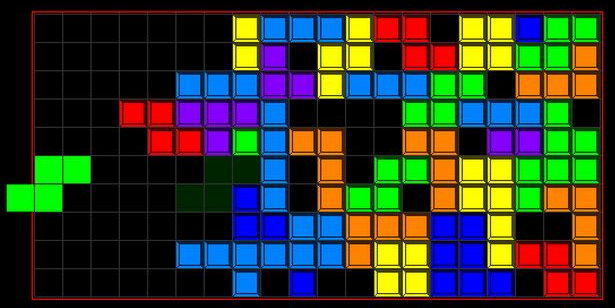
\includegraphics[width=0.65\textwidth]{images/chapter_5_evaluation/tetris_gaps}
    \centering~\caption{A bad attempt at playing Tetris\cite{tetris_gaps}.}
    \label{fig:chapter_5_evaluation-tetris_gaps}
\end{figure}

In conclusion, Table~\ref{table:analysis_results_throttle} and its ensuing analysis suggest that packet throttling is
\textbf{not} working as intended (despite showing some promise) and requires further improvement. Specifically, the
packet throttler needs a better mechanism to ``smooth out'' rough patches such that the aggregate bandwidth is
approximately in line with the configuration. The current algorithm applies a blanket delay to each packet that
passes through it and does not take into account the nuance that the pipeline might be experiencing low traffic. To
use Figure~\ref{fig:chapter_5_evaluation-tetris_gaps} as an analogy, the throttler needs to be better at packet
Tetris and minimise the time gaps between packets as to not overly throttle them.


\section{User Feedback}\label{section:user_feedback}

Six participants were generous enough to spend some of their time to road test Packet Courier and provide feedback.
Four of the participants took part in the user testing phase remotely and expressed their feedback via Microsoft
Forms\cite{microsoft_forms}; the other two provided their feedback in person, which enables notes to be taken as they
were observed interacting with the tool in addition to writing down their comments.

\subsection{Survey Results}\label{subsection:survey_results}

Participants were asked to download a \texttt{.zip} file of the repository before compiling Packet Courier and
completing a selection of tasks. Each of the questions was carefully worded as not to invoke any biases and gave only
the bare minimum context for solving the particular problem. The rationale behind this is that Packet Courier's
\texttt{README.md} should provide users with all the necessary context and troubleshooting information they might
need. Thus, if any of the participants were finding certain tasks unintuitive in a way that the \texttt{README.md}
was failing to address, then this is hugely useful feedback. Conversely, if the survey held their hand during the
entire process, then this defeats the point of collecting feedback on how easy to use and intuitive Packet Courier is
as a tool.

\begin{enumerate}
    \item \textbf{Please describe your occupation, i.e.: Computing Student, Computing Teacher, Network Engineer,
        etc.} \\
    Of the four participants, two where computing students, one was a software engineer and the other a game developer.
    \item \textbf{What platform will you be using to run Packet Courier?} \\
    Two participants were using Windows, one was using MacOS and the other Windows Subsystem for Linux.
    \item \textbf{Packet Courier needs to be compiled using Maven. How would this affect your motivation to use the
    tool? If you are indifferent, please select 5. (Scale from 0 to 10)} \\
    Three participants selected 3; one selected 8. Clearly the choice of project management tool was not particularly
    interesting to the participants.
    \item \textbf{Packet Courier can either be used as a library or executed as a program from the command line. In
    both cases Java 8 (or higher) is required. How would this affect your motivation to use the tool? If you are
    indifferent, please select 5. (Scale from 0 to 10)} \\
    Responses varied quite substantially with participants giving scores of 4, 7, 8 and 10. On the whole, it would
    seem as though participants liked the idea of Packet Courier using Java 8.
    \item \textbf{Packet Courier has no other prerequisites. How would this affect your motivation to use the tool?
    If you are indifferent, please select 5. (Scale from 0 to 10)} \\
    One participant selected 8 while the other three gave a score of 10. It would seem that using software with
    minimal dependencies is a massive upside for users, possibly because of how rare it is for complex tooling such
    as Packet Courier.
    \item \textbf{Please read the Introduction section of the \texttt{README}. Does it concisely convey the purpose
    of the tool and what makes it unique?} \\
    The responses to this question, 7, 8, 8 and 10, would indicate that \texttt{README} introduction is clear and
    informative with a little room for improvement.
    \item \textbf{Please write down any comments or criticisms regarding the Introduction section of the
    \texttt{README}. Is there anything missing? Is anything unclear or ambiguous?} \\
    Participants left a variety of comments in this section, ranging from \emph{``no''} to \emph{``could be a little
    more direct/plain (and therefore shorter)''}. One participant claimed that \emph{``the introduction is clear,
        with enough technical detail that users can understand what is happening but not so much detail that it would
        exclude those with lesser knowledge''}, with another saying that \emph{``uniqueness is not self evident''}
    but that \emph{``a section of the \texttt{README} explaining its benefits over other tools is unnecessary and
    self-indulgent''}. Whilst there is no clear consensus on this particular point (with some of it being down to
    taste), it might be worth investigating ways to trim down the \texttt{README} introduction so that users can get
    stuck straight into the tool. The comments about uniqueness are interesting, perhaps implying that users don't care
    about the unique selling point of a tool by the time they're skimming through the \texttt{README} and that they
    just want
    to get to work actually using it.
    \item \textbf{Please build the project. How complicated did you find this process?} \\
    All participants responded 10 to this prompt, reinforcing the choice to use Maven as the project management tool
    due to its simplicity.
    \item \textbf{Please explain any difficulties you had compiling Packet Courier.} \\
    Only one participant opted to leave a common here and suggested that the \texttt{README} mentions Maven's quiet
    mode to reduce console noise.
    \item \textbf{Please read \texttt{cmd\_example1.courierconfig}. On first glance, does this file read intuitively
    for a network emulation configuration? Suppose you were shown this file for the first time and were only told
    that it was used to configure an emulated network scenario; how well would you understand what the attributes and
    their values were referring to? If you can't find it, then the \texttt{README} should prove helpful.} \\
    Participants responded with scores of 8, 9, 9 and 10, indicating that the \texttt{.courierconfig} file format is
    very user friendly, even to people who are totally new to Packet Courier.
    \item \textbf{If you had to consult the \texttt{README} to get a better understanding of
    \texttt{cmd\_example1.courierconfig}, then please rate how helpful it was in clarifying any initial confusion.} \\
    Three participants opted to respond to this prompt, all giving a 10 rating.
    \item \textbf{Please write down any comments or criticisms regarding the structure or the contents of
    \texttt{cmd\_example1.courierconfig}. Did the \texttt{README} do a good job at explaining any components that
    weren't self
    evident in their function?} \\
    Two participants suggested that a YAML\cite{yaml} file would make for a cleaner, more human-readable format,
    which seems like a very sensible suggestion. Another participant noted that they had to read up on what
    \emph{``wall-clock''} meant, although the \texttt{README} did help them on that front.
    \item \textbf{Please run a Packet Courier emulation from the command-line using
    \texttt{cmd\_example1.courierconfig} as the configuration. How complicated did you find this process? Note that
    the network code for this configuration uses \texttt{python3}, and is known to work with version 3.8.10.} \\
    Participants gave scores of 7, 8, 10 and 10 for this section. So far it seems as though Packet Courier is being
    received as a very easy to use and highly intuitive tool.
    \item \textbf{Please explain any difficulties you had running a Packet Courier emulation.} \\
    The participants had a lot to say in response to this prompt. \\ \\
    Windows users experienced issues at the level of the operating system whereby double-quotes were stripped from
    Java \texttt{ProcessBuilder} commands\cite{java_ProcessBuilder_double_quote_windows,
        microsoft_docs_main_function}, which in turn prevented the Python scripts from properly parsing the
    arguments. Even after hot-fixing that problem, the Windows kernel seemed to block the packets as a security
    measure. These issues are not bugs or problems with Packet Courier specifically, but operating system quirks that
    must be worked around and troubleshot. The security/firewalling issue can be investigated and discussed in the
    \texttt{README} to help Windows users get the most out of the tool as quickly as possible. \\ \\
    The MacOS user cites that whilst their Packet Courier instance did technically start, it exited nearly
    immediately due to an attempt to bind an ip-address to an existing socket. This is a genuine design oversight
    that has been logged as a known bug. Packet Courier should instead attempt to bind its public and private
    ip-addresses to a socket and retry if they fail instead of presuming that they will succeed. \\ \\
    The WSL user managed to run the simulation in full but expressed how the \texttt{README} was lacking in its
    explanation of how to add loggers to the configuration. They also noted that Packet Courier doesn't create
    missing directories for features such as file logging and crash dumps, which would be a nice quality of life
    improvement.
    \item \textbf{Please briefly examine the simple\_client.py and simple\_server.py scripts that are run as part of
    \texttt{cmd\_example1.courierconfig}. Does the terminal output match what you would expect given the nature of
    the network code and the configuration file? Perhaps consider the order of the messages, as well as if any are
    missing.} \\
    One participant left a long response to this prompt, mentioning how \emph{``I am confused as to why sometimes Bob
    receives a message before Alice seems to have sent it''}. This is a largely unavoidable consequence of multiple
    processes competing for the same console output, however it should probably be mentioned somewhere in the
    \texttt{README}. The participant also suggests \emph{``perhaps more useful log in file form would to have
    separate files for each command node with a timestamp for each line''} since it \emph{``would allow easier side
    to side comparison on a specific message basis''}, which is undoubtedly another excellent feature proposition.
    \item \textbf{What are your general impressions of Packet Courier having used it? (Out of 5 possible stars)} \\
    Participants scored Packet Courier at an average of 4.25 stars.
    \item \textbf{How well do you think your actual experience of Packet Courier matches up to the description given
    in the Introduction of the \texttt{README}?} \\
    Two participants gave Packet Courier a 6/10 on this front, with the other two scored it 8 and 9 respectively.
    This is a surprising outcome in light of previous feedback and it is difficult to pinpoint what is motivating
    this score.
    \item \textbf{If you ever needed to emulate a network scenario, how likely do you think you would be to use
    Packet Courier as your tool of choice?} \\
    Participants gave pleasing ratings on this question: 7, 8, 9 and 10. This paints a picture that even despite the
    technical issues faced by some of the users, they were impressed enough by the presentation of the tool and
    understood its potential enough to overlook issues that could be fairly easily solved.
    \item \textbf{If you'd be hesitant to use Packet Courier again in the future, please explain why.} \\
    One participant left a comment for this prompt, claiming: \\
    \emph{``The lack of a GUI can be daunting for complex structures (e.g. multiple layers of nested topologies) but
    certainly not impossible. As mentioned I haven't seen alternatives but this most certainly does the job it claims
    with great flexibility.''} \\
    Whilst a GUI would certainly address this problem, it would require a significant amount of time and resources to
    develop for a set of fairly niche edge cases. It makes for a compelling suggestion, althougn some research into
    the demand for that kind of functionality might be useful.
    \item \textbf{Please write down any comments or criticisms regarding your experience of Packet Courier as a
    whole.} \\
    The most significant response to this prompt was: \\
    \emph{``As its biggest weakness is in troubleshooting the configuration, and linking with my previous feedback,
        perhaps a GUI tool/form/companion with rigid choices that generates a correct config file could be a useful
        extension.''}
\end{enumerate}

One of the participants went to the extra effort of configuring a couple of emulation scenarios from scratch and
documenting their experience. They said that Packet Courier was \emph{``overall easy to configure''} but had
difficulty debugging mistakes they had made when writing their configurations due to a number of unhelpful error
messages. For example, they had forgotten to place a comma between elements when defining a list of joint-mesh
topologies, to which Packet Courier spat out the following error: \texttt{Configuration error: com.google.protobuf
.InvalidProtocolBufferException: Repeated field elements cannot be null in field: thorpe.luke.network.simulation
.JointMeshTopologyProto.jointTopologies}. Whilst this is a Google Protocol Buffer parser exception rather than an
error message specifically programmed by the Packet Courier APIs, it still plays a role in user experience and thus
should be duly noted. The participant suggests that Packet Courier should use a parser that ignores trailing commas,
since most tooling they had worked with afford the users the luxury of not needing to delimit their lists. This may
be an option, but switching over to a YAML format would negate this problem entirely.

The overall consensus from the survey feedback suggests that users found Packet Courier easy to set up and run due to
a mixture of straightforward tooling, intuitive configuration files and clear documentation. However, there are
issues on Windows and MacOS that prevented some users from running emulations. Despite the fact that Java itself is
largely platform agnostic (and thus Packet Courier did actually \emph{run}), it seems as though the platform-specific
user space APIs do not always manifest themselves uniformly across all operating systems, i.e.: Windows stripping
process commands of double quotes and blocking packets. This is all useful feedback that will inform how Packet
Courier should be developed going forward in Section~\ref{section:future_work}.

\subsection{Observation Results}\label{subsection:observation_results}

Two user observation sessions were conducted to monitor how users \emph{behaved} while interacting with Packet Courier
before interviewing them to get an understanding for their thought processes\cite{user_observation}. The first
interview was done with ``John'' in a more informal manner in attempt to assess what users might expect from the tool
when reading the documentation and example configurations for the first time. The second interview was done more
formally with ``Harry'' to see how a user might debug a network protocol using Packet Courier\footnote{``John'' and
``Harry'' are aliases being used to preserve anonymity.}.

\subsubsection{John}\label{subsubsection:john}

John has a first class degree in computer science and now works as a full time junior software and DevOps engineer.

John was provided with a laptop at the start of the session with an IDE and a WSL terminal open at the root of the
Packet Courier repository. He was also was told that there was a \texttt{README.md} file in the root of the project
directory and was then asked to run an example configuration. John was reasonably comfortable with Java and Maven
since he had done some development with them at university so had Packet Courier built and running fairly quickly. He
was able to identify where the example configurations were based on the \texttt{README}, but said that running them
was \emph{``a bit fiddly''} due to how long the file paths were. The example configurations are buried fairly deep
inside the directory structure of the project and this could definitely be changed to make them more accessible.

John immediately went to run \texttt{cmd\_example1.courierconfig} which suggests that the naming of the example files
is intuitive, i.e.: \texttt{cmd\_example1.courierconfig} is the simplest configuration that can be run from the
command line. He was then prompted to look inside the file he had just run to see if it matched up to what he had
observed on the console. His initial reaction was that \emph{``it looks as though about half of the packets got
dropped, so seems on point''}. John had not even been asked whether he understood the contents of the
\texttt{.courierconfig}; he was instantly able to identify at a glance that about 50\% of the packets travelling from
Alice to Bob were supposed to be dropped. John then reran the simulation to see if it behaved consistently. He
confirmed that whilst the output was non-deterministic, the behaviour of Alice and Bob was still commensurate with
his expectations based on the configuration. He was not put off at all by the fact that sometimes Bob would appear to
receive packets ``before'' Alice, since he understood that the console output was not necessarily running perfectly
in tandem with the underlying client and server processes. In this way, John had built a very strong intuition for
the semantics of Packet Courier quite quickly.

John began to tinker around with the configuration, namely changing the drop probability to 0.9. He was confused to
see that Bob hadn't received any of the packets that Alice had sent. He reran the configuration to find the same
outcome. He then tried running the configuration with a drop probability of 0.3 and found that whilst Bob was
receiving packets from Alice, they were, by eye, less than John would have expected. He then concluded that Packet
Courier must have some kind of packet dropping bug and summarised his experience as follows:
\begin{quote}
    \emph{``I think [Packet Courer] is quite intuitive to use. The configs are quite readable and flexible, in that
    you don't need to fill [a configuration file] with the same amount of complexity each time. It behaves
    consistently and mostly as I would have expected, but there was that weird edge case with the super high and
    super low drops. It could have also benefited from a UI.''}
\end{quote}

Naturally it was disappointing to hear a user conclude that Packet Courier's drop mechanism is buggy given the rigour
of the unit and system testing conducted in Sections~\ref{section:unit_testing} and~\ref{section:system_testing}. The
behaviour that John had uncovered was then promptly investigated. As expected, the root cause of this erroneous
behaviour did not lie within the Packet Courier framework, but was instead a fragility issue in the way Alice and
Bob's connection had been set up in \texttt{cmd\_example1.courierconfig}, the details of which were discussed with
Harry in Section~\ref{subsubsection:harry}. In this way John's feedback had proved invaluable since his curiosity had
led him to discover a hidden edge case in \texttt{cmd\_example1.courierconfig}. Although this was not the result of a
Packet Courier bug, it is still problematic to provide users with examples that could easily convince them that the
framework itself is broken, so this configuration must be made more robust. Otherwise, John seemed to take to using
the tool like a duck to water, with the minor exception of struggling to type out the long path to the example
configurations. 

\subsubsection{Harry}\label{subsubsection:harry}

TODO


\section{Analysis of Objectives}\label{section:analysis_of_objectives}

\subsection{Network Topology Design Interface}\label{subsection:network_topology_design_interface}

\textbf{Objective 1: }\emph{An interface to design an arbitrary network topology.}

\subsection{Network Conditions Configuration Suite}\label{subsection:network_conditions_configuration_suite }

\textbf{Objective 2: }\emph{A configuration suite to define how packets are manipulated during message-passing.}

\subsection{Simulation of a Distributed Algorithm}\label{subsection:simulation_of_a_distributed_algorithm}

\textbf{Objective 3: }\emph{A mechanism to run a distributed algorithm across a virtual network topology which
reflects the
properties described by the user as per objectives 1) and 2).}

\subsection{Platform Agnosticism}\label{subsection:platform_agnosticism}

\textbf{Objective 4.a: }\emph{Basic usage of the tool should not depend on the operating system or hardware being used
.} \\ \\
\textbf{Objective 4.b: }\emph{Users should not be pigeonholed into working with a particular programming language in
order to
simulate their solution.}

\subsection{Plug-and-playability}\label{subsection:plug_and_playability}

\textbf{Objective 5.a: }\emph{Users should need minimal domain-specific knowledge in order to use the full set of
features on offer.} \\ \\
\textbf{Objective 5.b: }\emph{The prospective tool should be able to mimic a real network in a way that minimises
bespoke set-up, i.e.: if a user normally tests their distributed algorithm using real computers connected over a
physical network, then transitioning to using the prospective tool should be more or less seamless.}



%chapter 6 formatting


    \chapter{Conclusion}
    \pagestyle{fancy}
    \fancyhf{}
    \rhead{\small Conclusion}
    \lhead{\small Chapter 6}
    \rfoot{\thepage}
    \lfoot{\small MEng Project}
    \renewcommand{\headrulewidth}{2pt}
    \renewcommand{\footrulewidth}{2pt}
    In the early stages of Packet Courier's development, the mission statement was \emph{``to provide those with a
curiosity for distributed computer systems with the means to tinker around with network technologies as though they
were running in the real world''}. In fact, it was this very motto that inspired the more formal objectives defined
in Section~\ref{section:objectives}. Hopefully this report has done its due diligence to demonstrate beyond all doubt
that Packet Courier is a tool that truly embodies this sentiment. It provides developers, network engineers and
students alike to fine tune a network exactly to their liking and let their algorithms loose in a way that is
self-contained, realistic and resource inexpensive. Packet Courier has also proven to be a high-calibre piece of
software, insofar as it can emulate 100 nodes exchanging 5,000 packets per second in real time without so much as
adding 1ms of overhead latency to each packet (on the right hardware, of course). Many would consider a framework
capable of these feats to be worthy of usage in serious software and network engineering ventures.

Although Packet Courier was found to have demonstrably achieved most of its objectives in
Section~\ref{section:analysis_of_objectives}, there was ample scope for improvement. A mixture of prospective
features, performance improvements, documentation enhancements and bugfixes lie ahead in Packet Courier's future,
especially given that it will be released as an open source project on the 21\textsuperscript{st} of June 2022.


\section{Future Work}\label{section:future_work}

TODO



%chapter 7 formatting


    \chapter{Acknowledgements}
    \pagestyle{fancy}
    \fancyhf{}
    \rhead{\small Acknowledgements}
    \lhead{\small Chapter 7}
    \rfoot{\thepage}
    \lfoot{\small MEng Project}
    \renewcommand{\headrulewidth}{2pt}
    \renewcommand{\footrulewidth}{2pt}
    This section is reserved exclusively for the acknowledgements of technical contributions to this report that could
not be traditionally cited via the bibliography.

The LaTeX template for the report is based off of H. A. Ansari's M.Phil thesis, which can be found here:
\url{https://www.overleaf.com/latex/templates/m-dot-phil-thesis-format-sample-centre-of-excellence-in-solid-state-physics-university-of-the-punjab-lahore-pakistan/vqgzgjpxmwry}
[Accessed 20/06/2022]

The Vancouver referencing file used for this report, \texttt{unsrtnat.bst}, was written by P. W. Daly and can be
found here: \url{http://tug.ctan.org/tex-archive/macros/latex/contrib/natbib/unsrtnat.bst} [Accessed 20/06/2022]

The Google Protocol Buffer syntax highlighter for LaTeX used for this report was written by H. Lerchl and can be
found here: \url{https://github.com/aytchell/latex-listings-protobuf} [Accessed 20/06/2022]



%%chapter x formatting
%    \chapter{Write Your Xth Chapter's Name}
%    \pagestyle{fancy}
%    \fancyhf{}
%    \rhead{\small Write Your Xth Chapter's Name}
%    \lhead{\small Chapter X}
%    \rfoot{\thepage}
%    \lfoot{\small MEng Project}
%    \renewcommand{\headrulewidth}{2pt}
%    \renewcommand{\footrulewidth}{2pt}
%    \section{Write Here Your First Section Heading}
\hspace{4em}
Text in the first section. Text in the first section.Text in the first section.Text in the first section.Text in the first section.Text in the first section.Text in the first section.Text in the first section.Text in the first section.
Text in the first section.Text in the first section.Text in the first section.Text in the first section.Text in the first section.Text in the first section.Text in the first section.Text in the first section.Text in the first section.

\subsection{Write Here Your First Subsection Heading}
\hspace{4em}
Text in the subsection.Text in the subsection.Text in the subsection.Text in the subsection.Text in the subsection.Text in the subsection.Text in the subsection.Text in the subsection.
Text in the subsection.Text in the subsection.Text in the subsection.Text in the subsection.Text in the subsection.Text in the subsection.Text in the subsection.Text in the subsection.Text in the subsection.Text in the subsection.


\section{Write Here Your Second Section Heading}
\hspace{4em}
Text in the second section.Text in the second section.Text in the second section.Text in the second section.Text in the second section.Text in the second section.Text in the second section.Text in the second section.Text in the second section.Text in the second section.Text in the second section.Text in the second section.Text in the second section.Text in the second section.Text in the second section.Text in the second section.Text in the second section.

\subsection{Write Here Your Second Subsection Heading}
\hspace{4em}
Text in the second section.Text in the second section.Text in the second section.Text in the second section.Text in the second section.Text in the second section.Text in the second section.Text in the second section.Text in the second section.Text in the second section.Text in the second section.Text in the second section.Text in the second section.Text in the second section.Text in the second section.Text in the second section.Text in the second section.


\section{How to write an equation}
To add any Equation in document following environment needed.
\begin{equation}
    \textbf{Lattice Constant} =\frac{\lambda}{2\sin{\theta}}\sqrt{h^2+k^2+l^2}
    \label{eq 1.1}
\end{equation}
We can label any equation or figure using the command of  \begin{verbatim}
  \label{eq 1.1}
\end{verbatim}
Similarly, we can refer any equation, figure, and figure using the command of\begin{verbatim}
  \ref{eq 1.1}
\end{verbatim}


\section{Inserting Image}
To insert any image in the document follow the following environment.
\begin{figure}[hbt!]
    \centering
    
\includegraphics[width=2in,height=3in]{images/cover/icl_crest}
    \caption{Imperial College London Crest}
    \label{fig:my_label}
\end{figure}


\section{Table Formation}
\begin{table}[hbt!]
    \centering
    \caption{Caption of the Table}
    \begin{tabular}{ccc}
        \hline
        First Entry & Second Entry & Third Entry \\
        \hline
        item 11     & item 12      & item 13     \\
        item 21     & item 22      & item 23     \\
        \hline
    \end{tabular}
    \label{tab 1.1}
\end{table}


\section{Citation Example}
\hspace{4em}
Here some references are cited in APA style. \cite{vellacheri2014high} and \cite{asaithambi2021synthesis}



    \bibliography{bibliography}

\end{document}
